%definira klasu dokumenta 
\documentclass[12pt]{report} 

%prostor izmedu naredbi \documentclass i \begin{document} se zove uvod. U njemu se nalaze naredbe koje se odnose na cijeli dokument

%osnovni LaTex ne može riješiti sve probleme, pa se koriste različiti paketi koji olakšavaju izradu željenog dokumenta
\usepackage[croatian]{babel} 
\usepackage{amssymb}
\usepackage{amsmath}
\usepackage{txfonts}
\usepackage{mathdots}
\usepackage{titlesec}
\usepackage{array}
\usepackage{lastpage}
\usepackage{etoolbox}
\usepackage{tabularray}
\usepackage{color, colortbl}
\usepackage{adjustbox}
\usepackage{geometry}
\usepackage[classicReIm]{kpfonts}
\usepackage{hyperref}
\usepackage{fancyhdr}
\usepackage{multicol}
\usepackage{graphicx}
\usepackage{listings}
\graphicspath{{./prilozi}}

\usepackage{float}
\usepackage{setspace}
\restylefloat{table}


\patchcmd{\chapter}{\thispagestyle{plain}}{\thispagestyle{fancy}}{}{} %redefiniranje stila stranice u paketu fancyhdr

%oblik naslova poglavlja
\titleformat{\chapter}{\normalfont\huge\bfseries}{\thechapter.}{20pt}{\Huge}
\titlespacing{\chapter}{0pt}{0pt}{40pt}


\linespread{1.3} %razmak između redaka

\geometry{a4paper, left=1in, top=1in,}  %oblik stranice

\hypersetup{ colorlinks, citecolor=black, filecolor=black, linkcolor=black,	urlcolor=black }   %izgled poveznice


%prored smanjen između redaka u nabrajanjima i popisima
\newenvironment{packed_enum}{
	\begin{enumerate}
		\setlength{\itemsep}{0pt}
		\setlength{\parskip}{0pt}
		\setlength{\parsep}{0pt}
	}{\end{enumerate}}

\newenvironment{packed_item}{
	\begin{itemize}
		\setlength{\itemsep}{0pt}
		\setlength{\parskip}{0pt}
		\setlength{\parsep}{0pt}
	}{\end{itemize}}




%boja za privatni i udaljeni kljuc u tablicama
\definecolor{LightBlue}{rgb}{0.9,0.9,1}
\definecolor{LightGreen}{rgb}{0.9,1,0.9}

%Promjena teksta za dugačke tablice
\DefTblrTemplate{contfoot-text}{normal}{Nastavljeno na idućoj stranici}
\SetTblrTemplate{contfoot-text}{normal}
\DefTblrTemplate{conthead-text}{normal}{(Nastavljeno)}
\SetTblrTemplate{conthead-text}{normal}
\DefTblrTemplate{middlehead,lasthead}{normal}{Nastavljeno od prethodne stranice}
\SetTblrTemplate{middlehead,lasthead}{normal}

%podesavanje zaglavlja i podnožja

\pagestyle{fancy}
\lhead{Programsko inženjerstvo}
\rhead{Moj Kvart}
\lfoot{Ronins}
\cfoot{stranica \thepage/\pageref{LastPage}}
\rfoot{\today}
\renewcommand{\headrulewidth}{0.2pt}
\renewcommand{\footrulewidth}{0.2pt}


\begin{document} 
	
	
	
	\begin{titlepage}
		\begin{center}
			\vspace*{\stretch{1.0}} %u kombinaciji s ostalim \vspace naredbama definira razmak između redaka teksta
			\LARGE Programsko inženjerstvo\\
			\large Ak. god. 2021./2022.\\
			
			\vspace*{\stretch{3.0}}
			
			\huge Moj Kvart\\
			\Large Dokumentacija, Rev. \textit{2}\\
			
			\vspace*{\stretch{12.0}}
			\normalsize
			Grupa: \textit{Ronins}\\
			Voditelj: \textit{Mihael Miličević}\\
			
			
			\vspace*{\stretch{1.0}}
			Datum predaje: \textit{14.1.2022.}\\
	
			\vspace*{\stretch{4.0}}
			
			Nastavnik: \textit{Nikolina Frid}\\
		
		\end{center}

	
	\end{titlepage}

	
	\tableofcontents


	\chapter{Dnevnik promjena dokumentacije}				
		
		\begin{longtblr}[
				label=none
			]{
				width = \textwidth, 
				colspec={|X[2]|X[13]|X[3]|X[3]|}, 
				rowhead = 1
			}
			\hline
			\textbf{Rev.}	& \textbf{Opis promjene/dodatka} & \textbf{Autori} & \textbf{Datum}\\[3pt] \hline
			0.1 & Napravljen predložak.	& Mihael Miličević & 19.10.2021.		\\[3pt] \hline
			0.2 & Dodani dionici u projektu, te aktori i njihovi funkcionalni zahtjevi.	& Mihael Miličević & 20.10.2021.		\\[3pt] \hline 
			0.3 & Dodani obrasci uporabe.	& Mihael Miličević, Tomislav Žiger & 24.10.2021.		\\[3pt] \hline 
			0.4 & Dodan opis projektnog zadatka.	& Mihael Miličević & 24.10.2021.		\\[3pt] \hline 
			0.4.1 & Dodani ostali zahtjevi.	& Tomislav Žiger & 27.10.2021.		\\[3pt] \hline 
			0.4.2 & Ispravak obrazaca uporabe.	& Mihael Miličević & 28.10.2021.		\\[3pt] \hline 
			0.4.3 & Dodani dijagrami obrazaca uporabe.	& Mihael Miličević, Tomislav Žiger & 3.11.2021.		\\[3pt] \hline 
			0.4.4 & Dodani sekvencijski dijagrami.	& Mihael Miličević, Tomislav Žiger & 3.11.2021.		\\[3pt] \hline 
			0.5 & Dodana specifikacija baze podataka.	& Andrija Banić & 3.11.2021.	\\[3pt] \hline 
			0.5.1 & Dodan opis arhitekture sustava.	& Mihael Miličević & 8.11.2021.	\\[3pt] \hline 
			0.5.2 & Dodan dijagram razreda.	& Danijel Barišić, Mihael Miličević, Tomislav Žiger & 11.11.2021.	\\[3pt] \hline 
			
			0.5.3 & Dorađeni dijagrami razreda.	& Mihael Miličević, Tomislav Žiger & 14.11.2021.	\\[3pt] \hline 
			
			\textbf{1.0} & Verzija prve predaje. & Mihael Miličević & 14.11.2021. 		\\[3pt] \hline	
			
			1.1 & Dodan dijagram razmještaja.	& Mihael Miličević & 29.12.2021.	\\[3pt] \hline 
			
			1.2 & Dodan dijagram komponenti.	& Mihael Miličević & 29.12.2021.	\\[3pt] \hline 
			
			1.3 & Dodan dijagram aktivnosti.	& Mihael Miličević & 29.12.2021.	\\[3pt] \hline 
			1.4 & Dodan dijagram stanja.	& Mihael Miličević & 29.12.2021.	\\[3pt] \hline 
			
			% \textbf{1.0} & Verzija samo s bitnim dijelovima za 1. ciklus & * & 11.09.2013. \\[3pt] \hline 
			% \textbf{2.0} & Konačni tekst predloška dokumentacije  & * & 28.09.2013. \\[3pt] \hline 
			% &  &  & \\[3pt] \hline	
		\end{longtblr}
	\chapter{Opis projektnog zadatka}
		
	Cilj ovog projekta je razviti web aplikaciju pod nazivom "MojKvart" koja će omogućiti poboljšanje komunikacije i razmjenu informacije među stanovnicima jednog kvarta. Sama web aplikacija se sastoji od tri glavna dijela: "Forum", "Događaji" i "Vijeće četvrti", te postoje tri primarne vrste korisnika: "Obični stanovnik", "Vijećnik" i "Moderator". Dodatno postoji i uloga "Administrator", iako administratori nisu stanovnici niti jedne četvrti, nego je njihova uloga održavanje sustava.
	
	Svaki stanovnik četvrti koji poželi koristiti aplikaciju će prvo morati stvoriti korisnički račun. Kada otvori aplikaciju, prikazat će mu se stranica "Prijava". S obzirom da on trenutno nema korisnički račun, odabrat će opciju "Registracija", i to će preusmjeriti na stranicu na kojoj će morati ispuniti obrazac za stvaranje korisničkog računa. U obrascu će morati unijeti svoje ime, prezime, adresu stanovanja i adresu e-pošte, i pritom će ga se u sustavu raspoznavati primarno po njegovoj adresi e-pošte. Dodatno morat će odabrati i lozinku. Ukoliko pri registraciji korisnik odabere e-mail s kojim je već povezan neki korisnički račun u sustavu, ili ne unese sve podatke, ili unese neki podatak u krivom formatu (npr. napiše ime ili prezime malim slovom, ili za adresu unese adresu koja nije validna), dobit će prikladnu poruku o pogrešci, i tada će moći ispraviti te podatke i ponovno pokušati dovršiti registraciju. Ako se uspješno registrira, sustav će automatski po njegovoj adresi prepoznati kojem kvartu pripada, i preusmjerit će ga na početnu stranicu njegovog kvarta.
	
	Svaki korisnik koji ima korisnički račun će se na stranici "Prijava" moći prijaviti u sustav i time dobiti pristup korisničkom dijelu sustava tako da unese svoj e-mail i lozinku. Ukoliko korisnik napravi neku pogrešku u ovom koraku, recimo unese e-mail s kojim nije povezan niti jedan korisnički račun u sustavu, ili unese lozinku koja nije ispravna, dobit će prikladnu poruku o pogrešci, i tada će moći ispraviti tražene podatke i ponovno se pokušati prijaviti. Ako se uspješno prijavi, bit će preusmjeren na početnu stranicu svog kvarta.
	\chapter{Specifikacija programske potpore}
		
	\section{Funkcionalni zahtjevi}
			
			\noindent \textbf{Dionici:}
			
			\begin{packed_enum}
				
				\item Vlasnik (naručitelj)
				\item Stanovnik četvrti			
				\begin{packed_enum}
					\item  Obični stanovnik
					\item  Vijećnik
					\item  Moderator
				\end{packed_enum}
				\item Administrator	
				\item Razvojni tim
				
			\end{packed_enum}
			
			\noindent \textbf{Aktori i njihovi funkcionalni zahtjevi:}
			
			
			\begin{packed_enum}
			
				\item  \underbar{Neregistrirani korisnik (inicijator) može:}
				\begin{packed_enum}
					\item se registrirati u sustav stvaranjem novog korisničkog računa, za što su mu potrebni ime, prezime, adresa stanovanja, adresa e-pošte i lozinka
				\end{packed_enum}
				
				\item  \underbar{Neprijavljeni korisnik (inicijator) može:}
				\begin{packed_enum}
					\item se prijaviti u sustav,	za što su mu potrebni adresa e-pošte i lozinka
				\end{packed_enum}
				
				\item  \underbar{Stanovnik četvrti (inicijator) može:}
				\begin{packed_enum}
					\item čitati teme na "Forumu"
					\item otvarati teme na "Forumu"
					\item odgovarati u temama na "Forumu"
					\item uređivati svoje odgovore na "Forumu"
					\item ukloniti svoje odgovore na "Forumu"
					\item otvoriti temu na "Forumu" vezanu za objavu na "Vijeću četvrti", ako za tu objavu već nije otvorena tema
					\item čitati objave na "Vijeću četvrti"
					\item vidjeti najave događaja u cjelini "Događaji"
					\item predlagati najave budućih događaja u cjelini "Događaji", za što je potrebno navesti naziv, mjesto, vrijeme, trajanje i kratak opis
					\item poslati zahtjev administratorima za promjenu uloge (u "Vijećnika" ili "Moderatora")
					\item promijeniti osobne podatke	
					\item odjaviti se iz sustava
					\item obrisati svoj korisnički račun
				\end{packed_enum}
				
				\item  \underbar{Vijećnik (inicijator) može:}
				\begin{packed_enum}
					\item stvoriti objavu u cjelini "Vijeće četvrti"
					\item urediti objavu u cjelini "Vijeće četvrti"
					\item obrisati objavu u cjelini "Vijeće četvrti"	
				\end{packed_enum}
				
				\item  \underbar{Moderator (inicijator) može:}
				\begin{packed_enum}
					\item pregledati najave događanja koje predlažu stanovnici
					\item objaviti najave događanja u cjelini "Događaji"
					\item odbaciti prijedloge događanja
					\item urediti prijedloge događanja
					\item ukloniti odgovore u temama na "Forumu"
					\item ukloniti teme na Forumu
				\end{packed_enum}
				
				\item  \underbar{Administrator (inicijator) može:}
				\begin{packed_enum}
					\item vidjeti popis svih registriranih korisnika i njihove osobne podatke
					\item definirati četvrt i područje koje ta četvrt obuhvaća
					\item obrisati četvrti
					\item urediti podatke o četvrti
					\item vidjeti popis svih četvrti u sustavu
					\item odabrati pojedinu četvrt s popisa četvrti i pristupiti svom korisničkom sadržaju te četvrti
					\item pristupiti svim zahtjevima za uloge "Vijećnik" ili "Moderator"
					\item odbiti zahtjev za dodjelu uloge
					\item prihvatiti zahtjev za dodjelu uloge
					\item dodijeliti ulogu "Moderator" ili "Vijećnik" korisniku
					\item oduzeti ulogu "Moderator" ili "Vijećnik" korisniku
					\item privremeno blokirati korisnika
					\item pristupiti popisu blokiranih korisnika
					\item deblokirati korisnika
					\item trajno obrisati profil korisnika
				\end{packed_enum}
				
				\item  \underbar{Baza podataka (sudionik):}
				\begin{packed_enum}
					\item pohranjuje podatke o korisnicima i njihovim ovlastima
					\item pohranjuje podatke o četvrtima
					\begin{packed_enum}
						\item ulice koje im pripadaju
						\item teme na "Forumu"
						\item izvješća s "Vijeća četvrti"
					\end{packed_enum}
				\end{packed_enum}
				
			\end{packed_enum}
			
			\eject 
			
			
				
			\subsection{Obrasci uporabe}
					
					\noindent \underbar{\textbf{UC1 - Registracija}}
					\begin{packed_item}
	
						\item \textbf{Glavni sudionik: }Korisnik
						\item  \textbf{Cilj:} Stvoriti korisnički račun
						\item  \textbf{Sudionici:} Baza podataka
						\item  \textbf{Preduvjet:} -
						\item  \textbf{Opis osnovnog tijeka:}
						
						\item[] \begin{packed_enum}
	
							\item Korisnik odabire opciju "Registracija"
							\item Korisnik unosi tražene podatke - ime, prezime, adresa stanovanja, adresa e-pošte i lozinka
							\item Korisnik odabire opciju "Podnesi"
							\item Korisnik dobiva obavijest o uspješnoj registraciji
							\item Korisnik biva preusmjeren na početnu stranicu
						\end{packed_enum}
						
						\item  \textbf{Opis mogućih odstupanja:}
						
						\item[] \begin{packed_item}
	
							\item[3.a] Korisnik odabire e-mail s kojim je već povezan korisnički račun u sustavu, ili unese tražene podatke u krivom formatu
							\item[] \begin{packed_enum}
								
								\item Korisnik dobiva obavijest o pogrešci
								\item Korisnik mijenja podatke i ponovno odabire opciju "Podnesi", ili odustaje od registracije
								
							\end{packed_enum}
							
						\end{packed_item}
					\end{packed_item}
					
					\noindent \underbar{\textbf{UC2 - Prijava u sustav}}
					\begin{packed_item}
	
						\item \textbf{Glavni sudionik: }Korisnik
						\item  \textbf{Cilj:} Dobiti pristup korisničkom dijelu sustava
						\item  \textbf{Sudionici:} Baza podataka
						\item  \textbf{Preduvjet:} -
						\item  \textbf{Opis osnovnog tijeka:}
						
						\item[] \begin{packed_enum}
	
							\item Korisnik odabire opciju "Prijava"
							\item Korisnik unosi e-mail adresu i lozinku
							\item Korisnik odabire opciju "Podnesi"
							\item Korisnik dobiva pristup korisničkom dijelu sustava
							\item Korisnik biva preusmjeren na početnu stranicu
						\end{packed_enum}
						
						\item  \textbf{Opis mogućih odstupanja:}
						
						\item[] \begin{packed_item}
	
							\item[3.a] Korisnik unosi e-mail s kojim nije povezan niti jedan korisnički račun, ili unosi krivu lozinku, ili unosi tražene podatke u krivom formatu
							\item[] \begin{packed_enum}
								
								\item Korisnik dobiva obavijest o pogrešci
								\item Korisnik mijenja podatke i ponovno odabire opciju "Podnesi", ili odustaje od prijave
								
							\end{packed_enum}
							
						\end{packed_item}
					\end{packed_item}
					
					
					\noindent \underbar{\textbf{UC3 - Odjava iz sustava}}
					\begin{packed_item}
	
						\item \textbf{Glavni sudionik: }Korisnik
						\item  \textbf{Cilj:} Odjaviti se iz sustava
						\item  \textbf{Sudionici:} -
						\item  \textbf{Preduvjet:} Korisnik je prijavljen u sustav
						\item  \textbf{Opis osnovnog tijeka:}
						
						\item[] \begin{packed_enum}
	
							\item Korisnik odabire opciju "Odjava"
							\item Korisnik gubi pristup korisničkom dijelu sustava
							\item Korisnik biva preusmjeren na stranicu "Prijava"
						\end{packed_enum}
					\end{packed_item}					
					
					
					\noindent \underbar{\textbf{UC4 - Pregled osobnih podataka}}
					\begin{packed_item}
	
						\item \textbf{Glavni sudionik: }Korisnik
						\item  \textbf{Cilj:} Vidjeti osobne podatke
						\item  \textbf{Sudionici:} Baza podataka
						\item  \textbf{Preduvjet:} Korisnik je prijavljen u sustav
						\item  \textbf{Opis osnovnog tijeka:}
						
						\item[] \begin{packed_enum}
	
							\item Korisnik odabire opciju "Osobni podaci"
							\item Korisnik biva preusmjeren na stranicu "Osobni podaci" gdje dobije prikaz svojih osobnih podataka
						\end{packed_enum}
					\end{packed_item}
					
					\noindent \underbar{\textbf{UC5 - Promjena osobnih podataka}}
					\begin{packed_item}
	
						\item \textbf{Glavni sudionik: }Korisnik
						\item  \textbf{Cilj:} Promijeniti osobne podatke
						\item  \textbf{Sudionici:} Baza podataka
						\item  \textbf{Preduvjeti:}
						\item[] \begin{packed_enum}
							\item Korisnik je prijavljen u sustav
							\item Korisnik pregledava svoje osobne podatke (UC4)
						\end{packed_enum}
						\item  \textbf{Opis osnovnog tijeka:}
						
						\item[] \begin{packed_enum}
	
							\item Korisnik odabire opciju "Promjena osobnih podataka"
							\item Korisnik mijenja svoje podatke
							\item Korisnik odabire opciju "Spremi promjene"
							\item Baza podataka se ažurira
							\item Korisnik biva preusmjeren na stranicu "Osobni podaci"
						\end{packed_enum}
						
						\item  \textbf{Opis mogućih odstupanja:}
						
						\item[] \begin{packed_item}
	
							\item[3.a] Korisnik mijenja svoje osobne podatke, ali ne spremi promjene
							\item[] \begin{packed_enum}
								
								\item Sustav upozori korisnika da nije spremio promjene
								\item Korisnik spremi promjene, ili odustane od njih
								
							\end{packed_enum}
							
							\item[3.b] Korisnik pokuša promijeniti e-mail adresu
							\item[] \begin{packed_enum}
								
								\item Sustav upozori korisnika da ne može promijeniti e-mail adresu
								\item Korisnik promijeni neke druge osobne podatke, ili odustane od promjena
								
							\end{packed_enum}
							
							\item[3.c] Korisnik pokuša promijeniti neki osobni podatak u nedozvoljeni format (npr. ime koje počinje malim slovom), ili pokuša promijeniti adresu na neku adresu koja ne postoji u sustavu
							\item[] \begin{packed_enum}
								
								\item Sustav upozori korisnika o pogrešci
								\item Korisnik pokuša promijeniti svoje osobne podatke u ispravan format, ili odustane od promjena
								
							\end{packed_enum}
							
						\end{packed_item}
					\end{packed_item}
					
					\noindent \underbar{\textbf{UC6 - Brisanje korisničkog računa}}
					\begin{packed_item}
	
						\item \textbf{Glavni sudionik: }Korisnik
						\item  \textbf{Cilj:} Obrisati korisnički račun
						\item  \textbf{Sudionici:} Baza podataka
						\item  \textbf{Preduvjeti:}
						\item[] \begin{packed_enum}
							\item Korisnik je prijavljen u sustav
							\item Korisnik pregledava svoje osobne podatke (UC4)
							\item Korisnik nema ulogu "Administrator"
						\end{packed_enum}
						\item  \textbf{Opis osnovnog tijeka:}
						
						\item[] \begin{packed_enum}
	
							\item Korisnik odabire opciju "Obriši korisnički račun"
							\item Sustav upozori korisnika da je brisanje korisničkog računa trajna i nepovratna akcija
							\item Korisnik potvrđuje svoj odabir
							\item Korisnički račun se izbriše iz baze podataka
							\item Korisnik biva preusmjeren na stranicu "Prijava"
							
						\end{packed_enum}
						
						\item  \textbf{Opis mogućih odstupanja:}
						
						\item[] \begin{packed_item}
	
							\item[3.a] Korisnik odustane od brisanja svog računa
							\item[] \begin{packed_enum}
								
								\item Korisnik biva preusmjeren na stranicu "Osobni podaci"
														
							\end{packed_enum}
							
						\end{packed_item}
					\end{packed_item}
					
					\noindent \underbar{\textbf{UC7 - Promjena kvarta stanovanja korisnika}}
					\begin{packed_item}
	
						\item \textbf{Glavni sudionik: }Korisnik
						\item  \textbf{Cilj:} Ukloniti dodatne uloge ("Vijećnik" i "Moderator") korisniku koji je promijenio kvart
						\item  \textbf{Sudionici:} Baza podataka
						\item  \textbf{Preduvjeti:}
						\item[] \begin{packed_enum}
							\item Korisnik je prijavljen u sustav
							\item Korisnik je promijenio svoje osobne podatke (UC5)
							\item Korisnik je pri promjeni osobnih podataka promijenio adresu, i nova adresa ne pripada kvartu kojem je pripadala njegova stara adresa
						\end{packed_enum}
						\item  \textbf{Opis osnovnog tijeka:}
						
						\item[] \begin{packed_enum}
	
							\item Sustav korisniku oduzima uloge "Moderator" i "Vijećnik", ako ih ima
							\item Baza podataka se ažurira
						\end{packed_enum}
					\end{packed_item}
					
					
					\noindent \underbar{\textbf{UC8 - Promjena adrese radi ispravljanja nevažećeg statusa stanovanja}}
                    \begin{packed_item}
    
                        \item \textbf{Glavni sudionik: }Korisnik
                        \item  \textbf{Cilj:} Promijeniti adresu i omogućiti korisniku pristup korisničkom dijelu sustava
                        \item  \textbf{Sudionici:} Baza podataka
                        \item  \textbf{Preduvjeti:}
						\item[] \begin{packed_enum}
							\item Korisnik je prijavljen u sustav
							\item Korisnikov status stanovanja je "Nevažeći"
						\end{packed_enum}
                        \item  \textbf{Opis osnovnog tijeka:}
                        
                        \item[] \begin{packed_enum}
    
                            \item Korisnik ispunjava obrazac u kojem unosi novu adresu
                            \item Korisnik odabire opciju "Spremi promjene"
                            \item Baza podataka se ažurira
                            \item Korisnik biva preusmjeren na početnu stranicu
                        \end{packed_enum}
                        
                        \item  \textbf{Opis mogućih odstupanja:}
                        
                        \item[] \begin{packed_item}
    
                            \item[2.a] Korisnik nije unio novu adresu, ili je adresa koju je korisnik unio nevažeća
                            \item[] \begin{packed_enum}
                                
                                \item Sustav upozorava korisnika o pogrešci
                                \item Korisnik ispravlja pogrešku i ponovno odabire opciju "Spremi promjene", ili odustaje od popravljanja adrese
                                
                            \end{packed_enum}
                            
                        \end{packed_item}
                    \end{packed_item}					
					

					\noindent \underbar{\textbf{UC9 - Pregled događaja u cjelini "Događaji" }}
					\begin{packed_item}
	
						\item \textbf{Glavni sudionik: }Korisnik
						\item  \textbf{Cilj:} Prikaz potvrđenih događaja u korisnikovom kvartu
						\item  \textbf{Sudionici:} Baza podataka
						\item  \textbf{Preduvjet:} Korisnik je prijavljen u sustav
						\item  \textbf{Opis osnovnog tijeka:}
						
						\item[] \begin{packed_enum}
	
							\item Korisnik odabere opciju "Događaji"
							\item Korisnik biva preusmjeren na stranicu "Događaji" gdje dobije prikaz potvrđenih događaja u njegovom kvartu
						\end{packed_enum}
						
							
						\end{packed_item}
					\noindent \underbar{\textbf{UC10 - Stvaranje prijedloga događaja}}
					\begin{packed_item}
	
						\item \textbf{Glavni sudionik: }Korisnik
						\item  \textbf{Cilj:} Stvoriti prijedlog događaja
						\item  \textbf{Sudionici:} Baza podataka
						\item  \textbf{Preduvjeti:}
						\item[] \begin{packed_enum}
							\item Korisnik je prijavljen u sustav
							\item Korisnik pregledava događaje (UC8)
						\end{packed_enum}
						\item  \textbf{Opis osnovnog tijeka:}
						
						\item[] \begin{packed_enum}
	
							\item Korisnik odabire opciju "Novi prijedlog događaja" 
							\item Korisnik ispunjava polja "naziv", "mjesto", "vrijeme", "trajanje" i "kratki opis"
							\item Korisnik odabire opciju "Objavi prijedlog događaja"
							\item Baza podataka se ažurira
						\end{packed_enum}
						
						\item  \textbf{Opis mogućih odstupanja:}
						
						\item[] \begin{packed_item}
	
							\item[3.a] Korisnik nije ispunio sva polja prilikom stvaranja prijedloga događaja
							\item[] \begin{packed_enum}
								
								\item Sustav upozori korisnika da sva polja nisu ispunjena
								\item Korisnik ispuni preostala polja i odabire opciju "Objavi prijedlog događaja", ili odustane od prijedloga
							\end{packed_enum}
								
							\item[3.b] Korisnik pokuša napustiti stranicu prije biranja opcije "Objavi prijedlog događaja"
							\item[] \begin{packed_enum}
								
								\item Sustav upozori korisnika da se skica prijedloga događaja neće spremiti
								\item Korisnik odabire opciju "Objavi prijedlog događaja", ili odustaje od objave prijedloga događaja
								
							\end{packed_enum}
							
							
						\end{packed_item}
					\end{packed_item}						
					\noindent \underbar{\textbf{UC11 - Pregled prijedloga događaja}}
					\begin{packed_item}
	
						\item \textbf{Glavni sudionik: }Moderator
						\item  \textbf{Cilj:} Pregled prijedloga događaja u cjelini "Događaji"
						\item  \textbf{Sudionici:} Baza podataka
						\item  \textbf{Preduvjeti:}
						\item[] \begin{packed_enum}
							\item Korisnik je prijavljen u sustav
							\item Korisnik ima ulogu "Moderator"
							\item Korisnik pregledava događaje (UC8)
						\end{packed_enum}
						\item  \textbf{Opis osnovnog tijeka:}
						
						\item[] \begin{packed_enum}
	
							\item Korisnik odabire opciju "Prijedlozi događaja" 
							\item Korisnik biva preusmjeren na stranicu "Prijedlozi događaja" gdje dobije prikaz svih prijedloga događaja za svoj kvart
							
						\end{packed_enum}
						\end{packed_item}
						
						\noindent \underbar{\textbf{UC12 - Uređivanje prijedloga događaja}}
					\begin{packed_item}
	
						\item \textbf{Glavni sudionik: }Moderator
						\item  \textbf{Cilj:} Uređivanje prijedloga događaja u cjelini "Događaji"
						\item  \textbf{Sudionici:} Baza podataka
						\item  \textbf{Preduvjeti:}
						\item[] \begin{packed_enum}
							\item Korisnik je prijavljen u sustav
							\item Korisnik ima ulogu "Moderator"
							\item Korisnik pregledava prijedloge događaja (UC10)
						\end{packed_enum}
						\item  \textbf{Opis osnovnog tijeka:}
						
						\item[] \begin{packed_enum}
	
							\item Korisnik odabire prijedlog događaja 
							\item Korisnik odabire opciju "Uredi prijedlog događaja"
							\item Korisnik uređuje polja za odabrani prijedlog događaja
							\item Korisnik odabire opciju "Spremi promjene"
							\item Baza podataka se ažurira
							
						\end{packed_enum}
						\item  \textbf{Opis mogućih odstupanja:}
						
						\item[] \begin{packed_item}
	
							\item[4.a] Korisnik nije spremio promjene
							\item[] \begin{packed_enum}
								
								\item Sustav upozori korisnika da promjene nisu spremljene
								\item Korisnik odabire opciju "Spremi promjene", ili odustane od promjena
								
							\end{packed_enum}
							
							\item[4.b] Korisnik obriše neko polje, tj. ostavi ga praznim nakon unošenja promjena
							\item[] \begin{packed_enum}
								
								\item Sustav upozori korisnika da niti jedno polje u formularu ne može biti prazno
								\item Korisnik ispuni to polje i odabire opciju "Spremi promjene", ili odustane od promjena
								
							\end{packed_enum}
							
							
						\end{packed_item}
						\end{packed_item}
					\noindent \underbar{\textbf{UC13 - Objava prijedloga događaja}}
					\begin{packed_item}
	
						\item \textbf{Glavni sudionik: }Moderator
						\item  \textbf{Cilj:} Objava predloženog događaja u cjelini "Događaji"
						\item  \textbf{Sudionici:} Baza podataka
						\item  \textbf{Preduvjeti:}
						\item[] \begin{packed_enum}
							\item Korisnik je prijavljen u sustav
							\item Korisnik ima ulogu "Moderator"
							\item Korisnik pregledava prijedloge događaja (UC10)
						\end{packed_enum}
						\item  \textbf{Opis osnovnog tijeka:}
						
						\item[] \begin{packed_enum}
	
							\item Korisnik odabire prijedlog događaja 
							\item Korisnik odabire opciju "Objavi događaj"
							\item Baza podataka se ažurira
							
						\end{packed_enum}
						\end{packed_item}
					\noindent \underbar{\textbf{UC14 - Brisanje prijedloga događaja}}
					\begin{packed_item}
	
						\item \textbf{Glavni sudionik: }Moderator
						\item  \textbf{Cilj:} Brisanje prijedloga događaja u cjelini "Događaji"
						\item  \textbf{Sudionici:} Baza podataka
						\item  \textbf{Preduvjeti:}
						\item[] \begin{packed_enum}
							\item Korisnik je prijavljen u sustav
							\item Korisnik ima ulogu "Moderator"
							\item Korisnik pregledava prijedloge događaja (UC10)
						\end{packed_enum}
						\item  \textbf{Opis osnovnog tijeka:}
						
						\item[] \begin{packed_enum}
	
							\item Korisnik odabire prijedlog događaja 
							\item Korisnik odabire opciju "Obriši prijedlog događaja"
							\item Baza podataka se ažurira
							
						\end{packed_enum}
						
					\end{packed_item}
					\noindent \underbar{\textbf{UC15 - Pregled tema na "Forumu"}}
					\begin{packed_item}
	
						\item \textbf{Glavni sudionik: }Korisnik
						\item  \textbf{Cilj:} Prikaz tema na "Forumu"
						\item  \textbf{Sudionici:} Baza podataka
						\item  \textbf{Preduvjet:} Korisnik je prijavljen u sustav
						\item  \textbf{Opis osnovnog tijeka:}
						
						\item[] \begin{packed_enum}
	
							\item Korisnik odabire cjelinu „Forum“
							\item Korisnik biva preusmjeren na stranicu "Forum" gdje gdje dobije prikaz tema na "Forumu", poredanih po vremenu zadnjeg odgovora
							
						\end{packed_enum}
						
						
					\end{packed_item}						
					\noindent \underbar{\textbf{UC16 - Prikaz teme na "Forumu"}}
					\begin{packed_item}
	
						\item \textbf{Glavni sudionik: }Korisnik
						\item  \textbf{Cilj:} Odabrati temu na "Forumu" i vidjeti sve objave u njoj
						\item  \textbf{Sudionici:} Baza podataka
						\item  \textbf{Preduvjeti:}
						\item[] \begin{packed_enum}
							\item Korisnik je prijavljen u sustav
							\item Korisnik pregledava "Forum" (UC14)
						\end{packed_enum}
						\item  \textbf{Opis osnovnog tijeka:}
						
						\item[] \begin{packed_enum}
	
							\item Korisnik u cjelini "Forum" odabire željenu temu
							\item Prikazuje se odabrana tema
							
						\end{packed_enum}
						
					\end{packed_item}
					
					
					\noindent \underbar{\textbf{UC17 - Otvaranje teme na "Forumu"}}
                    \begin{packed_item}
    
                        \item \textbf{Glavni sudionik: }Korisnik
                        \item  \textbf{Cilj:} Otvoriti temu na "Forumu"
                        \item  \textbf{Sudionici:} Baza podataka
                        \item  \textbf{Preduvjeti:}
						\item[] \begin{packed_enum}
							\item Korisnik je prijavljen u sustav
							\item Korisnik pregledava "Forum" (UC14)
						\end{packed_enum}
                        \item  \textbf{Opis osnovnog tijeka:}
                        
                        \item[] \begin{packed_enum}
    
                            \item Korisnik odabire opciju "Otvori novu temu"
                            \item Korisnik ispunjava obrazac s imenom novootvorene teme i prvom objavom u toj temi
                            \item Korisnik odabire opciju "Otvori temu"
                            \item Baza podataka se ažurira
                            \item Korisnik biva preusmjeren na stranicu koja odgovara novootvorenoj temi
                        \end{packed_enum}
                        
                        \item  \textbf{Opis mogućih odstupanja:}
						
						\item[] \begin{packed_item}
						\item[3.a] Korisnik nije ispunio sva polja u obrascu s imenom i prvom objavom u temi
							\item[] \begin{packed_enum}
								
								\item Sustav upozorava korisnika da mora ispuniti sva polja u obrascu
								\item Korisnik ispunjava polja i ponovno odabire opciju "Otvori temu", ili odustaje od otvaranja teme
								
							\end{packed_enum}
                    		\end{packed_item}	
                    	\end{packed_item}				
					
					\noindent \underbar{\textbf{UC18 - Odgovaranje na objavu u temi na "Forumu"}}
					\begin{packed_item}
	
						\item \textbf{Glavni sudionik: }Korisnik
						\item  \textbf{Cilj:} Odgovoriti na željenu objavu u temi na "Forumu"
						\item  \textbf{Sudionici:} Baza podataka
						\item  \textbf{Preduvjeti:}
						\item[] \begin{packed_enum}
							\item Korisnik je prijavljen u sustav
							\item Korisnik pregledava temu na "Forumu" (UC15)
						\end{packed_enum}
						\item  \textbf{Opis osnovnog tijeka:}
						
						\item[] \begin{packed_enum}
	
							\item Korisnik unutar teme na "Forumu" na odabranoj objavi odabire opciju "Odgovori"
							\item Otvara se polje za odgovor
							\item Korisnik ispunjava polje za odgovor tekstom
							\item Korisnik bira opciju "Objavi odgovor"
							\item Baza podataka se ažurira
							\item Korisnik biva preusmjeren na stranicu koja odgovara toj temi na "Forumu"
							
							
						\end{packed_enum}
						
						\item  \textbf{Opis mogućih odstupanja:}
						
						\item[] \begin{packed_item}
						\item[3.a] Korisnik pokuša objaviti odgovor bez teksta
							\item[] \begin{packed_enum}
								
								\item Sustav upozorava korisnika da odgovor na "Forumu" ne može biti prazan tekst
								\item Korisnik doda tekst u polje za tekst odgovora, ili odustane od objave odgovora
								
							\end{packed_enum}
						
						
					\end{packed_item}
					\end{packed_item}
					\noindent \underbar{\textbf{UC19 - Uređivanje odgovora u temi na "Forumu"}}
					\begin{packed_item}
	
						\item \textbf{Glavni sudionik: }Korisnik
						\item  \textbf{Cilj:} Uređivanje odgovora u temi na "Forumu" 
						\item  \textbf{Sudionici:} Baza podataka
						\item  \textbf{Preduvjeti:}
						\item[] \begin{packed_enum}
							\item Korisnik je prijavljen u sustav
							\item Korisnik pregledava temu na "Forumu" (UC15)
							\item Korisnik je autor odgovora kojeg odabire
						\end{packed_enum}
						\item  \textbf{Opis osnovnog tijeka:}
						
						\item[] \begin{packed_enum}
	
							\item Korisnik odabire opciju "Uredi odgovor"
							\item Otvara se polje za odgovor koje sadrži trenutnu verziju teksta odgovora
							\item Korisnik uređuje tekst
							\item Korisnik odabire opciju "Spremi promjene"
							\item Baza podataka se ažurira
							\item Korisnik biva preusmjeren na stranicu koja odgovara toj temi na "Forumu"
							
						\end{packed_enum}
							
						\item  \textbf{Opis mogućih odstupanja:}
						
						\item[] \begin{packed_item}
						\item[4.a] Korisnik napušta stranicu iako uređeni odgovor nije objavio
							\item[] \begin{packed_enum}
								
								\item Sustav upozorava korisnika da uređeni tekst neće biti spremljen ako napusti stranicu
								\item Korisnik odabire opciju "Spremi promjene", ili odustane od promjena
								
							\end{packed_enum}
						\item[4.b] Korisnik je obrisao sav tekst odgovora i odabrao opciju "Spremi promjene"
							\item[] \begin{packed_enum}
								
								\item Sustav upozorava korisnika da tekst objave ne smije biti prazan
								\item Korisnik u polje za tekst odgovora doda neki tekst, ili odustane od promjene odgovora
								
							\end{packed_enum}
						\end{packed_item}
						
					\end{packed_item}	
					
					\noindent \underbar{\textbf{UC20 - Brisanje odgovora u temi na "Forumu"}}
					\begin{packed_item}
	
						\item \textbf{Glavni sudionik: }Korisnik
						\item  \textbf{Cilj:} Obrisati odgovor u temi na "Forumu"
						\item  \textbf{Sudionici:} Baza podataka
						\item  \textbf{Preduvjeti:}
						\item[] \begin{packed_enum}
							\item Korisnik je prijavljen u sustav
							\item Korisnik pregledava temu na "Forumu" (UC15)
							\item Korisnik odabire odgovor čiji autor je on, ili korisnik ima ulogu "Moderator"
						\end{packed_enum}
						\item  \textbf{Opis osnovnog tijeka:}
						
						\item[] \begin{packed_enum}
	
							\item Korisnik pronalazi odgovor koji želi obrisati
							\item Korisnik odabire opciju "Izbriši odgovor"
							\item Sustav upozorava korisnika da je brisanje odgovora trajna i nepovratna akcija
							\item Korisnik potvrđuje svoj odabir
							\item Baza podataka se ažurira
							\item Korisnik biva preusmjeren na stranicu koja odgovara toj temi na "Forumu"
							
							
						\end{packed_enum}
						
						\item  \textbf{Opis mogućih odstupanja:}
						
						\item[] \begin{packed_item}
						\item[4.a] Korisnik odustane od brisanja odgovora
							\item[] \begin{packed_enum}
								
								\item Prozor za brisanje odgovora se ugasi
								
							\end{packed_enum}
						\end{packed_item}
						
						
					\end{packed_item}
					
					\noindent \underbar{\textbf{UC21 - Brisanje teme na "Forumu"}}
					\begin{packed_item}
	
						\item \textbf{Glavni sudionik: }Moderator
						\item  \textbf{Cilj:} Obrisati temu na "Forumu"
						\item  \textbf{Sudionici:} Baza podataka
						\item  \textbf{Preduvjeti:}
						\item[] \begin{packed_enum}
							\item Korisnik je prijavljen u sustav
							\item Korisnik pregledava "Forum" (UC14)
							\item Korisnik ima ulogu "Moderator"
						\end{packed_enum}
						\item  \textbf{Opis osnovnog tijeka:}
						
						\item[] \begin{packed_enum}
	
							\item Korisnik odabire opciju "Obriši temu"
							\item Sustav upozorava korisnika da je brisanje teme trajna i nepovratna akcija
							\item Korisnik potvrđuje svoju odluku i tema se obriše
							\item Baza podataka se ažurira
							\item Korisnik biva preusmjeren na stranicu "Forum"
						\end{packed_enum}
						
						\item  \textbf{Opis mogućih odstupanja:}
						
						\item[] \begin{packed_item}
	
							\item[3.a] Korisnik odustane od brisanja teme
							\item[] \begin{packed_enum}
								
								\item Korisnik biva preusmjeren na stranicu "Forum"
								
							\end{packed_enum}
							
						\end{packed_item}
					\end{packed_item}
					
					\noindent \underbar{\textbf{UC22 - Automatsko brisanje teme na "Forumu"}}
                    \begin{packed_item}
    
                        \item \textbf{Glavni sudionik: }Korisnik
                        \item  \textbf{Cilj:} Obrisati temu na "Forumu" u kojoj je upravo izbrisan zadnji odgovor
                        \item  \textbf{Sudionici:} Baza podataka
                        \item  \textbf{Preduvjeti:}
						\item[] \begin{packed_enum}
							\item Korisnik je prijavljen u sustav
							\item Korisnik je upravo obrisao odgovor u temi na "Forumu" (UC18)
							\item Obrisani odgovor je bio posljednji odgovor u svojoj temi
						\end{packed_enum}
                        \item  \textbf{Opis osnovnog tijeka:}
                        
                        \item[] \begin{packed_enum}
    
                            \item Sustav automatski obriše tu temu na "Forumu"
                            \item Baza podataka se ažurira
                        \end{packed_enum}
                    \end{packed_item}
					
										
					\noindent \underbar{\textbf{UC23 - Pregled cjeline "Vijeće četvrti" }}
					\begin{packed_item}
	
						\item \textbf{Glavni sudionik: }Korisnik
						\item  \textbf{Cilj:} Pregled svih izvješća u cjelini "Vijeće četvrti"
						\item  \textbf{Sudionici:} Baza podataka
						\item  \textbf{Preduvjet:} Korisnik je prijavljen u sustav
						\item  \textbf{Opis osnovnog tijeka:}
						
						\item[] \begin{packed_enum}
	
							\item Korisnik odabire opciju "Vijeće četvrti" 
							\item Korisnik biva preusmjeren na stranicu "Vijeće četvrti" gdje dobije prikaz svih izvješća, poredanih kronološki od najsvježijeg
							
							
						\end{packed_enum}

						
					\end{packed_item}		
					
					\noindent \underbar{\textbf{UC24 - Prikaz izvješća u "Vijeću četvrti" }}
					\begin{packed_item}
	
						\item \textbf{Glavni sudionik: }Korisnik
						\item  \textbf{Cilj:} Prikaz jednog izvješća u cjelini "Vijeće četvrti"
						\item  \textbf{Sudionici:} Baza podataka
						\item  \textbf{Preduvjeti:}
						\item[] \begin{packed_enum}
							\item Korisnik je prijavljen u sustav
							\item Korisnik pregledava "Vijeće četvrti" (UC20)
						\end{packed_enum}
						\item  \textbf{Opis osnovnog tijeka:}
						
						\item[] \begin{packed_enum}
	
							\item Korisnik odabire izvješće koje želi pregledati 
							\item Korisnik biva preusmjeren na stranicu koja odgovara izvješću koje je odabrao
							
							
						\end{packed_enum}

						
					\end{packed_item}							
								
					\noindent \underbar{\textbf{UC25 - Objava novog izvješća na "Vijeću četvrti"}}
					\begin{packed_item}
	
						\item \textbf{Glavni sudionik: }Vijećnik
						\item  \textbf{Cilj:} Objaviti novo izvješće na "Vijeću četvrti"
						\item  \textbf{Sudionici:} Baza podataka
						\item  \textbf{Preduvjeti:}
						\item[] \begin{packed_enum}
							\item Korisnik je prijavljen u sustav
							\item Korisnik pregledava "Vijeće četvrti" (UC20)
							\item Korisnik ima ulogu "Vijećnik"
						\end{packed_enum}
						\item  \textbf{Opis osnovnog tijeka:}
						
						\item[] \begin{packed_enum}
	
							\item Korisnik odabire opciju "Stvaranje novog izvješća" 
							\item Otvara se polje za pisanje izvješća
							\item Korisnik ispunjava polje tekstom izvješća
							\item Korisnik odabire opciju "Objavi izvješće"
							\item Baza podataka se ažurira
							\item Korisnik biva preusmjeren na stranicu "Vijeća četvrti"
							
							
						\end{packed_enum}
						
						\item  \textbf{Opis mogućih odstupanja:}
						
						\item[] \begin{packed_item}
	
							\item[4.a] Korisnik pokuša objaviti prazno izvješće bez teksta
							\item[] \begin{packed_enum}
								
								\item Sustav upozorava korisnika da izvješće s "Vijeća četvrti" ne može biti prazan tekst
								\item Korisnik doda tekst u polje za tekst izvješća, ili odustane od objave izvješća
							\end{packed_enum}
								
							\item[4.b] Korisnik pokuša napustiti stranicu bez biranja opcije "Objavi izvješće"
							\item[] \begin{packed_enum}
								
								\item Sustav upozorava korisnika da skica izvješća neće biti objavljena
								\item Korisnik odabire opciju "Objavi izvješće", ili odustaje od objave
								
							\end{packed_enum}
							
						\end{packed_item}
						
						
					\end{packed_item}					
					\noindent \underbar{\textbf{UC26 - Uređivanje izvješća na "Vijeću četvrti"}}
					\begin{packed_item}
	
						\item \textbf{Glavni sudionik: }Vijećnik
						\item  \textbf{Cilj:} Urediti izvješće
						\item  \textbf{Sudionici:} Baza podataka
						\item  \textbf{Preduvjeti:}
						\item[] \begin{packed_enum}
							\item Korisnik je prijavljen u sustav
							\item Korisnik pregledava izvješće s "Vijeća četvrti" (UC21)
							\item Korisnik ima ulogu "Vijećnik"
							\item Korisnik je autor izvješća kojeg pregledava
						\end{packed_enum}
						\item  \textbf{Opis osnovnog tijeka:}
						
						\item[] \begin{packed_enum}
	
							\item Korisnik odabire opciju "Uredi izvješće"
							\item Otvara se tekstualno polje koje sadrži trenutnu verziju izvješća
							\item Korisnik uređuje tekst
							\item Korisnik odabire opciju "Spremi promjene"
							\item Baza podataka se ažurira
							\item Korisnik biva preusmjeren na stranicu koja odgovara tom izvješću na "Vijeću četvrti"
							
							
							
						\end{packed_enum}
						\item  \textbf{Opis mogućih odstupanja:}
						
						\item[] \begin{packed_item}
						\item[4.a] Korisnik napušta stranicu iako uređeno izvješće nije objavio
							\item[] \begin{packed_enum}
								
								\item Sustav upozorava korisnika da uređeni tekst neće biti spremljen ako napusti stranicu
								\item Korisnik odabire opciju "Spremi promjene", ili odustane od promjena
								
							\end{packed_enum}
							
						\item[4.b] Korisnik je obrisao sav tekst izvješća i odabrao opciju "Spremi promjene"
							\item[] \begin{packed_enum}
								
								\item Sustav upozorava korisnika da tekst izvješća ne smije biti prazan
								\item Korisnik u polje za tekst izvješća doda neki tekst, ili odustane od promjene izvješća
								
							\end{packed_enum}
						\end{packed_item}
						
						
						
					\end{packed_item}					
					

					\noindent \underbar{\textbf{UC27 - Brisanje izvješća s "Vijeća četvrti"}}
					\begin{packed_item}
	
						\item \textbf{Glavni sudionik: }Vijećnik
						\item  \textbf{Cilj:} Obrisati izvješće u cjelini "Vijeće četvrti"
						\item  \textbf{Sudionici:} Baza podataka
						\item  \textbf{Preduvjeti:}
						\item[] \begin{packed_enum}
							\item Korisnik je prijavljen u sustav
							\item Korisnik pregledava izvješće s "Vijeća četvrti" (UC21)
							\item Korisnik ima ulogu "Vijećnik"														\end{packed_enum}
						\item  \textbf{Opis osnovnog tijeka:}
						
						\item[] \begin{packed_enum}
	
							\item Korisnik odabire opciju "Obriši izvješće"
							\item Sustav upozorava korisnika da je brisanje izvješća trajna i nepovratna akcija
							\item Korisnik potvrđuje svoju odluku i izvješće se obriše
							\item Baza podataka se ažurira
							\item Korisnik biva preusmjeren na stranicu "Vijeće četvrti"
						\end{packed_enum}
						
						\item  \textbf{Opis mogućih odstupanja:}
						
						\item[] \begin{packed_item}
	
							\item[3.a] Korisnik odustane od brisanja izvješća
							\item[] \begin{packed_enum}
								
								\item Korisnik biva preusmjeren na stranicu koja odgovara tom izvješću
								
							\end{packed_enum}
							
						\end{packed_item}
					\end{packed_item}
						
						
						
					\noindent \underbar{\textbf{UC28 - Otvaranje teme na "Forumu" vezanu za izvješće s "Vijeća četvrti"}}
					\begin{packed_item}
	
						\item \textbf{Glavni sudionik: }Korisnik
						\item  \textbf{Cilj:} Na "Forumu" stvoriti temu vezanu uz izvješće na "Vijeću četvrti"
						\item  \textbf{Sudionici:} Baza podataka
						\item  \textbf{Preduvjeti:}
						\item[] \begin{packed_enum}
							\item Korisnik je prijavljen u sustav
							\item Korisnik pregledava izvješće s "Vijeća četvrti" (UC21)
							\item Za odabrano izvješće nije već otvorena tema na "Forumu"								\end{packed_enum}
						\item  \textbf{Opis osnovnog tijeka:}
						
						\item[] \begin{packed_enum}
	
							\item Korisnik odabire opciju "Otvori temu na 'Forumu'"
							\item Korisnik ispunjava obrazac s prvom objavom u novootvorenoj temi, za ime teme se automatski postavlja naslov izvješća, a kao nulta objava u novootvorenoj temi se postavlja tekst izvješća s autorom "Vijeće četvrti"
							\item Korisnik odabire opciju "Otvori temu"
							\item Otvara se nova tema na cjelini "Forum"
							\item Baza podataka se ažurira
							\item Korisnik biva preusmjeren na novootvorenu temu na "Forumu"
							
						\end{packed_enum}	
						
						\item  \textbf{Opis mogućih odstupanja:}
						
						\item[] \begin{packed_item}
						\item[3.a] Korisnik nije ispunio obrazac s prvom objavom u temi
							\item[] \begin{packed_enum}
								
								\item Sustav upozorava korisnika da mora ispuniti sva polja u obrascu
								\item Korisnik ispunjava polja i ponovno odabire opciju "Otvori temu", ili odustaje od otvaranja teme
								
							\end{packed_enum}
                    		\end{packed_item}				
						
					\end{packed_item}
					
					\noindent \underbar{\textbf{UC29 - Podnošenje zahtjeva za dodjelu uloge}}
					\begin{packed_item}
	
						\item \textbf{Glavni sudionik: }Korisnik
						\item  \textbf{Cilj:} Priložiti zahtjev za promjenu uloge
						\item  \textbf{Sudionici:} Baza podataka
						\item  \textbf{Preduvjeti:}
						\item[] \begin{packed_enum}
							\item Korisnik je prijavljen u sustav
							\item Korisnik nema ulogu za koju šalje zahtjev
							\item Korisnik pregledava svoje osobne podatke (UC4)
							\item Korisnik već nije predao zahtjev za ulogom koju sad traži čiji je status trenutno "Nerazriješen"
							\item Korisnik nema ulogu "Administrator"
							\end{packed_enum}
						\item  \textbf{Opis osnovnog tijeka:}
						
						\item[] \begin{packed_enum}
	
							\item Korisnik odabire opciju "Novi zahtjev za ulogom"
							\item Korisnik odabire ulogu za koju šalje zahtjev
							\item Korisnik pošalje zahtjev
							\item Baza podataka se ažurira
						\end{packed_enum}
						
						\item  \textbf{Opis mogućih odstupanja:}
						
						\item[] \begin{packed_item}
						
							\item[3.a] Korisnik pokuša poslati zahtjev bez da je odabrao ulogu
							\item[] \begin{packed_enum}
								
								\item Sustav upozori korisnika da nije odabrao ulogu
								\item Korisnik odabere ulogu, ili odustane od zahtjeva
								
							\end{packed_enum}
	
							\item[3.a] Korisnik pokuša ugasiti prozor za zahtjev za ulogu bez da je poslao zahtjev
							\item[] \begin{packed_enum}
								
								\item Sustav upozori korisnika da nije poslao zahtjev
								\item Korisnik pošalje zahtjev, ili odustane od njega
								
							\end{packed_enum}
							
						\end{packed_item}
					\end{packed_item}
					
					\noindent \underbar{\textbf{UC30 - Pristup svim korisnicima u sustavu}}
					\begin{packed_item}
	
						\item \textbf{Glavni sudionik: }Administrator
						\item  \textbf{Cilj:} Pristupiti popisu svih korisnika u sustavu
						\item  \textbf{Sudionici:} Baza podataka
						\item  \textbf{Preduvjeti:}
						\item[] \begin{packed_enum}
							\item Korisnik je prijavljen u sustav
							\item Korisnik ima ulogu "Administrator"
							\end{packed_enum}
						\item  \textbf{Opis osnovnog tijeka:}
						
						\item[] \begin{packed_enum}
	
							\item Korisnik odabire opciju "Korisnici"
							\item Korisnik biva preusmjeren na stranicu "Korisnici" gdje dobije popis svih korisnika sustava
						\end{packed_enum}
					
					\end{packed_item}
					
					\noindent \underbar{\textbf{UC31 - Pregled korisnika}}
					\begin{packed_item}
	
						\item \textbf{Glavni sudionik: } Administrator
						\item  \textbf{Cilj:} Pregledati osobne podatke korisnika (radi jednoznačnosti, u daljnjem tekstu: objekt)
						\item  \textbf{Sudionici:} Baza podataka
						\item  \textbf{Preduvjeti:}
						\item[] \begin{packed_enum}
							\item Korisnik je prijavljen u sustav
							\item Korisnik ima ulogu "Administrator"
							\item Korisnik pregledava sve korisnike u sustavu (UC27)
						\end{packed_enum}
						\item  \textbf{Opis osnovnog tijeka:}
						
						\item[] \begin{packed_enum}
	
							\item Korisnik odabire objekta čije osobne podatke želi pregledati
							\item Korisnik biva preusmjeren na stranicu s osobnim podacima objekta
						\end{packed_enum}
						
					\end{packed_item}
					
					\noindent \underbar{\textbf{UC32 - Dodjela uloge}}
					\begin{packed_item}
	
						\item \textbf{Glavni sudionik: }Administrator
						\item  \textbf{Cilj:} Dodijeliti ulogu korisniku (radi jednoznačnosti, u daljnjem tekstu: objekt)
						\item  \textbf{Sudionici:} Baza podataka
						\item  \textbf{Preduvjeti:}
						\item[] \begin{packed_enum}
							\item Korisnik je prijavljen u sustav
							\item Korisnik ima ulogu "Administrator"
							\item Korisnik pregledava osobne podatke objekta (UC28)
							\item Objekt nema ulogu koju mu korisnik želi dodijeliti
							\item Objekt nema ulogu "Administrator"
						\end{packed_enum}
						\item  \textbf{Opis osnovnog tijeka:}
						
						\item[] \begin{packed_enum}
	
							\item Korisnik odabire ulogu koju želi dodijeliti objektu
							\item Baza podataka se ažurira
							\item Korisnik biva preusmjeren na stranicu s osobnim podacima objekta
						\end{packed_enum}
						
					\end{packed_item}
					
					\noindent \underbar{\textbf{UC33 - Oduzimanje uloge}}
					\begin{packed_item}
	
						\item \textbf{Glavni sudionik: }Administrator
						\item  \textbf{Cilj:} Oduzeti ulogu korisniku (radi jednoznačnosti, u daljnjem tekstu: objekt)
						\item  \textbf{Sudionici:} Baza podataka
						\item  \textbf{Preduvjeti:}
						\item[] \begin{packed_enum}
							\item Korisnik je prijavljen u sustav
							\item Korisnik ima ulogu "Administrator"
							\item Korisnik pregledava osobne podatke objekta (UC28)
							\item Objekt ima ulogu koju mu korisnik želi oduzeti
							\item Objekt nema ulogu "Administrator"
						\end{packed_enum}
						\item  \textbf{Opis osnovnog tijeka:}
						
						\item[] \begin{packed_enum}
	
							\item Korisnik odabire ulogu koju želi oduzeti objektu
							\item Baza podataka se ažurira
							\item Korisnik biva preusmjeren na stranicu s osobnim podacima objekta
						\end{packed_enum}
						
					\end{packed_item}
					
					\noindent \underbar{\textbf{UC34 - Automatsko razrješavanje zahtjeva za ulogu kod manualne dodjele uloge korisniku}}
                    \begin{packed_item}
    
                        \item \textbf{Glavni sudionik: }Administrator
                        \item  \textbf{Cilj:} Promijeniti status zahtjeva za ulogu korisnika (radi jednoznačnosti, u daljnjem tekstu: objekt) u "Prihvaćen" pri manualnoj dodjeli uloge
                        \item  \textbf{Sudionici:} Baza podataka
                        \item  \textbf{Preduvjeti:}
						\item[] \begin{packed_enum}
							\item Korisnik je prijavljen u sustav
							\item Korisnik ima ulogu "Administrator"
							\item Korisnik je upravo objektu dodijelio ulogu (UC31)
							\item Postoji zahtjev za ulogom sa statusom "Nerazriješen" čiji autor je objekt i u kojem je uloga jednaka ulozi koju je korisnik manualno dodijelio objektu
						\end{packed_enum}
						\item  \textbf{Opis osnovnog tijeka:}
						
						\item[] \begin{packed_enum}
	
							\item Status zahtjeva za ulogu se automatski promijeni u "Prihvaćen"
							\item Baza podataka se ažurira
						\end{packed_enum}

                    \end{packed_item}
					
					\noindent \underbar{\textbf{UC35 - Pregled zahtjeva za ulogu}}
					\begin{packed_item}
	
						\item \textbf{Glavni sudionik: }Administrator
						\item  \textbf{Cilj:} Pregledati zahtjeve korisnika za uloge
						\item  \textbf{Sudionici:} Baza podataka
						\item  \textbf{Preduvjeti:}
						\item[] \begin{packed_enum}
							\item Korisnik je prijavljen u sustav
							\item Korisnik ima ulogu "Administrator"
						\end{packed_enum}
						\item  \textbf{Opis osnovnog tijeka:}
						
						\item[] \begin{packed_enum}
	
							\item Korisnik odabire opciju "Zahtjevi uloga"
							\item Korisnik biva preusmjeren na stranicu "Zahtjevi uloga" gdje dobije pregled svih nerazriješenih zahtjeva uloga
						\end{packed_enum}
						

					\end{packed_item}
					
					\noindent \underbar{\textbf{UC36 - Prihvaćanje zahtjeva za ulogu}}
					\begin{packed_item}
	
						\item \textbf{Glavni sudionik: } Administrator
						\item  \textbf{Cilj:} Prihvatiti zahtjev korisnika za ulogu
						\item  \textbf{Sudionici:} Baza podataka
						\item  \textbf{Preduvjeti:}
						\item[] \begin{packed_enum}
							\item Korisnik je prijavljen u sustav
							\item Korisnik ima ulogu "Administrator"
							\item Korisnik pregledava zahtjeve uloga (UC31)
						\end{packed_enum}
						\item  \textbf{Opis osnovnog tijeka:}
						
						\item[] \begin{packed_enum}
	
							\item Korisnik odabire zahtjev
							\item Korisnik odabire opciju "Prihvati"
							\item Baza podataka se ažurira
						\end{packed_enum}
						
					\end{packed_item}
					
					\noindent \underbar{\textbf{UC37 - Odbijanje zahtjeva za ulogu}}
					\begin{packed_item}
	
						\item \textbf{Glavni sudionik: } Administrator
						\item  \textbf{Cilj:} Odbiti zahtjev korisnika za ulogu
						\item  \textbf{Sudionici:} Baza podataka
						\item  \textbf{Preduvjeti:}
						\item[] \begin{packed_enum}
							\item Korisnik je prijavljen u sustav
							\item Korisnik ima ulogu "Administrator"
							\item Korisnik pregledava zahtjeve uloga (UC31)
						\end{packed_enum}
						\item  \textbf{Opis osnovnog tijeka:}
						
						\item[] \begin{packed_enum}
	
							\item Korisnik odabire zahtjev
							\item Korisnik odabire opciju "Odbij"
							\item Baza podataka se ažurira
						\end{packed_enum}
					
					\end{packed_item}
					
					\noindent \underbar{\textbf{UC38 - Pregled blokiranih korisnika}}
					\begin{packed_item}
	
						\item \textbf{Glavni sudionik: }Administrator
						\item  \textbf{Cilj:} Pregledati popis blokiranih korisnika
						\item  \textbf{Sudionici:} Baza podataka
						\item  \textbf{Preduvjeti:}
						\item[] \begin{packed_enum}
							\item Korisnik je prijavljen u sustav
							\item Korisnik ima ulogu "Administrator"
							\item Korisnik pregledava sve korisnike u sustavu (UC27)
						\end{packed_enum}
						\item  \textbf{Opis osnovnog tijeka:}
						
						\item[] \begin{packed_enum}
	
							\item Korisnik odabire opciju "Blokirani korisnici"
							\item Korisnik biva preusmjeren na stranicu gdje vidi popis blokiranih korisnika
						\end{packed_enum}
					
					\end{packed_item}
					
					\noindent \underbar{\textbf{UC39 - Blokiranje korisnika}}
					\begin{packed_item}
	
						\item \textbf{Glavni sudionik: }Administrator
						\item  \textbf{Cilj:} Blokirati korisnika (radi jednoznačnosti, u daljnjem tekstu: objekt)
						\item  \textbf{Sudionici:} Baza podataka
						\item  \textbf{Preduvjeti:}
						\item[] \begin{packed_enum}
							\item Korisnik je prijavljen u sustav
							\item Korisnik ima ulogu "Administrator"
							\item Korisnik pregledava osobne podatke objekta (UC28)
							\item Objekt trenutno nije blokiran
							\item Objekt nema ulogu "Administrator"
						\end{packed_enum}
						\item  \textbf{Opis osnovnog tijeka:}
						
						\item[] \begin{packed_enum}
	
							\item Korisnik odabire opciju "Blokiraj korisnika"
							\item Baza podataka se ažurira
							\item Korisnik biva preusmjeren na stranicu s osobnim podacima objekta
						\end{packed_enum}
						
					\end{packed_item}
					
					\noindent \underbar{\textbf{UC40 - Deblokiranje korisnika}}
					\begin{packed_item}
	
						\item \textbf{Glavni sudionik: }Administrator
						\item  \textbf{Cilj:} Deblokirati korisnika (radi jednoznačnosti, u daljnjem tekstu: objekt)
						\item  \textbf{Sudionici:} Baza podataka
						\item  \textbf{Preduvjeti:}
						\item[] \begin{packed_enum}
							\item Korisnik je prijavljen u sustav
							\item Korisnik ima ulogu "Administrator"
							\item Korisnik pregledava osobne podatke objekta (UC28)
							\item Objekt je trenutno blokiran
						\end{packed_enum}
						\item  \textbf{Opis osnovnog tijeka:}
						
						\item[] \begin{packed_enum}
	
							\item Korisnik odabire opciju "Deblokiraj korisnika"
							\item Baza podataka se ažurira
							\item Korisnik biva preusmjeren na stranicu s osobnim podacima objekta
						\end{packed_enum}
						
					\end{packed_item}
					
					\noindent \underbar{\textbf{UC41 - Brisanje korisničkog računa drugog korisnika}}
					\begin{packed_item}
	
						\item \textbf{Glavni sudionik: }Administrator
						\item  \textbf{Cilj:} Obrisati korisnički račun drugog korisnika (radi jednoznačnosti, u daljnjem tekstu: objekt)
						\item  \textbf{Sudionici:} Baza podataka
						\item  \textbf{Preduvjeti:}
						\item[] \begin{packed_enum}
							\item Korisnik je prijavljen u sustav
							\item Korisnik ima ulogu "Administrator"
							\item Korisnik pregledava osobne podatke objekta (UC28)
							\item Objekt nema ulogu "Administrator"
						\end{packed_enum}
						\item  \textbf{Opis osnovnog tijeka:}
						
						\item[] \begin{packed_enum}
	
							\item Korisnik odabire opciju "Obriši korisnički račun"
							\item Sustav upozorava korisnika da je brisanje korisničkog računa trajna i nepovratna akcija
							\item Korisnik potvrđuje svoj odabir i briše korisnički račun drugog korisnika
							\item Baza podataka se ažurira
							\item Korisnik biva preusmjeren na stranicu s popisom svih korisnika u sustavu
						\end{packed_enum}
						
						\item  \textbf{Opis mogućih odstupanja:}
						
						\item[] \begin{packed_item}
	
							\item[3.a] Korisnik odustane od brisanja korisničkog računa
							\item[] \begin{packed_enum}
								
								\item Korisnik biva preusmjeren na pregled osobnih podataka objekta							
							\end{packed_enum}
							
						\end{packed_item}
					\end{packed_item}
					
					\noindent \underbar{\textbf{UC42 - Pregled popisa kvartova}}
					\begin{packed_item}
	
						\item \textbf{Glavni sudionik: }Administrator
						\item  \textbf{Cilj:} Pregledati popis kvartova
						\item  \textbf{Sudionici:} Baza podataka
						\item  \textbf{Preduvjeti:}
						\item[] \begin{packed_enum}
							\item Korisnik je prijavljen u sustav
							\item Korisnik ima ulogu "Administrator"
						\end{packed_enum}
						\item  \textbf{Opis osnovnog tijeka:}
						
						\item[] \begin{packed_enum}
	
							\item Korisnik odabire opciju "Kvartovi"
							\item Korisnik biva preusmjeren na stranicu "Kvartovi" gdje vidi popis kvartova
						\end{packed_enum}
					
					\end{packed_item}
					
					\noindent \underbar{\textbf{UC43 - Pregled kvarta}}
					\begin{packed_item}
	
						\item \textbf{Glavni sudionik: }Administrator
						\item  \textbf{Cilj:} Pregledati korisnički sadržaj sustava za pojedini kvart
						\item  \textbf{Sudionici:} Baza podataka
						\item  \textbf{Preduvjeti:}
						\item[] \begin{packed_enum}
							\item Korisnik je prijavljen u sustav
							\item Korisnik ima ulogu "Administrator"
							\item Korisnik pregledava popis kvartova (UC38)
						\end{packed_enum}
						\item  \textbf{Opis osnovnog tijeka:}
						
						\item[] \begin{packed_enum}
	
							\item Korisnik odabire kvart koju želi pregledati
							\item Korisnik biva preusmjeren na početnu stranicu tog kvarta
						\end{packed_enum}
						
					\end{packed_item}
					
					\noindent \underbar{\textbf{UC44 - Definiranje kvarta}}
					\begin{packed_item}
	
						\item \textbf{Glavni sudionik: }Administrator
						\item  \textbf{Cilj:} Definirati novi kvart
						\item  \textbf{Sudionici:} Baza podataka
						\item  \textbf{Preduvjeti:}
						\item[] \begin{packed_enum}
							\item Korisnik je prijavljen u sustav
							\item Korisnik ima ulogu "Administrator"
							\item Korisnik pregledava popis kvartova (UC38)
						\end{packed_enum}
						\item  \textbf{Opis osnovnog tijeka:}
						
						\item[] \begin{packed_enum}
	
							\item Korisnik odabire opciju "Dodaj kvart"
							\item Korisnik ispunjava sve potrebne podatke - ime kvarta, imena ulica, za svaku ulicu raspon brojeva
							\item Korisnik odabire opciju "Spremi promjene"
							\item Baza podataka se ažurira
							\item Korisnik biva preusmjeren na stranicu "Kvartovi"
						\end{packed_enum}
						
						\item  \textbf{Opis mogućih odstupanja:}
						
						\item[] \begin{packed_item}
	
							\item[3.a] Korisnik unese ime kvarta koje je već zauzeto, ili ime ulice koje je već zauzeto, ili za kvart ne definira niti jednu ulicu, ili za neku ulicu ne definira raspon brojeva, ili za neku ulicu definira mogućnost postojanja negativnih brojeva
							\item[] \begin{packed_enum}
								
								\item Sustav obavještava korisnika o pogrešci
								\item Korisnik ispravlja pogrešku i odabire opciju "Spremi promjene", ili odustane od definiranja četvrti
								
							\end{packed_enum}
							
						\end{packed_item}
					\end{packed_item}
					
					\noindent \underbar{\textbf{UC45 - Uređivanje kvarta}}
					\begin{packed_item}
	
						\item \textbf{Glavni sudionik: }Administrator
						\item  \textbf{Cilj:} Promijeniti podatke o nekom kvartu
						\item  \textbf{Sudionici:} Baza podataka
						\item  \textbf{Preduvjeti:}
						\item[] \begin{packed_enum}
							\item Korisnik je prijavljen u sustav
							\item Korisnik ima ulogu "Administrator"
							\item Korisnik pregledava podatke o kvartu (UC39)
						\end{packed_enum}
						\item  \textbf{Opis osnovnog tijeka:}
						
						\item[] \begin{packed_enum}
	
							\item Korisnik odabire opciju "Uredi kvart"
							\item Korisnik stvara promjene
							\item Korisnik odabire opciju "Spremi promjene"
							\item Baza podataka se ažurira
							\item Korisnik biva preusmjeren na stranicu koja sadrži podatke o tom kvartu
						\end{packed_enum}
						
						\item  \textbf{Opis mogućih odstupanja:}
						
						\item[] \begin{packed_item}
	
							\item[3.a] Korisnik odustane od promjena
							\item[] \begin{packed_enum}
								
								\item Korisnik biva preusmjeren na stranicu koja sadrži podatke o tom kvartu
								
							\end{packed_enum}
							
						\end{packed_item}
					\end{packed_item}
					
					\noindent \underbar{\textbf{UC46 - Brisanje kvarta}}
					\begin{packed_item}
	
						\item \textbf{Glavni sudionik: }Administrator
						\item  \textbf{Cilj:} Obrisati kvart
						\item  \textbf{Sudionici:} Baza podataka
						\item  \textbf{Preduvjeti:}
						\item[] \begin{packed_enum}
							\item Korisnik je prijavljen u sustav
							\item Korisnik ima ulogu "Administrator"
							\item Korisnik pregledava podatke o kvartu (UC39)
						\end{packed_enum}
						\item  \textbf{Opis osnovnog tijeka:}
						
						\item[] \begin{packed_enum}
	
							\item Korisnik odabire opciju "Obriši kvart"
							\item Sustav upozorava korisnika da je brisanje kvarta trajna i nepovratna akcija
							\item Korisnik potvrđuje svoju odluku i obriše kvart
							\item Iz baze podataka se obrišu svi podaci vezani za taj kvart - sve teme na "Forumu", sva izvješća s "Vijeća četvrti", svi događaji na "Događajima"
							\item Baza podataka se ažurira
							\item Korisnik biva preusmjeren na stranicu "Kvartovi"
						\end{packed_enum}
						
						\item  \textbf{Opis mogućih odstupanja:}
						
						\item[] \begin{packed_item}
	
							\item[3.a] Korisnik odustane od brisanja kvarta
							\item[] \begin{packed_enum}
								
								\item Korisnik biva preusmjeren na stranicu koja sadrži podatke o tom kvartu
								
							\end{packed_enum}
							
						\end{packed_item}
					\end{packed_item}
					
					\noindent \underbar{\textbf{UC47 - Automatsko postavljanje statusa stanovanja korisnika na "Nevažeći"}}
                    \begin{packed_item}
    
                        \item \textbf{Glavni sudionik: }Administrator
                        \item  \textbf{Cilj:} Ažurirati status stanovanja korisnicima pri promjeni podataka ili brisanja kvarta
                        \item  \textbf{Sudionici:} Baza podataka
                        \item  \textbf{Preduvjeti:}
						\item[] \begin{packed_enum}
							\item Korisnik je prijavljen u sustav
							\item Korisnik ima ulogu "Administrator"
							\item Korisnik je promijenio podatke o kvartu (UC44) ili obrisao kvart (UC45)
							\item Postoje korisnici sustava čije adrese zbog prethodne točke preduvjeta su prestale biti važeće
						\end{packed_enum}
                        \item  \textbf{Opis osnovnog tijeka:}
                        
                        \item[] \begin{packed_enum}
    
                            \item Sustav automatski postavi status stanovanja na "Nevažeći" svim korisnicima čije adrese su zbog promjena podataka ili brisanja kvarta prestale biti važeće
                            \item Baza podataka se ažurira
                        \end{packed_enum}
                        
                    \end{packed_item}
						
				\subsubsection{Dijagrami obrazaca uporabe}
					
					\textit{Prikazati odnos aktora i obrazaca uporabe odgovarajućim UML dijagramom. Nije nužno nacrtati sve na jednom dijagramu. Modelirati po razinama apstrakcije i skupovima srodnih funkcionalnosti.}
				\eject		
				
			\subsection{Sekvencijski dijagrami}
				
				\textbf{\textit{dio 1. revizije}}\\
				
				\textit{Nacrtati sekvencijske dijagrame koji modeliraju najvažnije dijelove sustava (max. 4 dijagrama). Ukoliko postoji nedoumica oko odabira, razjasniti s asistentom. Uz svaki dijagram napisati detaljni opis dijagrama.}
				\eject
	
		\section{Ostali zahtjevi}
		
			\textbf{\textit{dio 1. revizije}}\\
		 
			 \textit{Nefunkcionalni zahtjevi i zahtjevi domene primjene dopunjuju funkcionalne zahtjeve. Oni opisuju \textbf{kako se sustav treba ponašati} i koja \textbf{ograničenja} treba poštivati (performanse, korisničko iskustvo, pouzdanost, standardi kvalitete, sigurnost...). Primjeri takvih zahtjeva u Vašem projektu mogu biti: podržani jezici korisničkog sučelja, vrijeme odziva, najveći mogući podržani broj korisnika, podržane web/mobilne platforme, razina zaštite (protokoli komunikacije, kriptiranje...)... Svaki takav zahtjev potrebno je navesti u jednoj ili dvije rečenice.}
			 
			 
			 
	
	\chapter{Arhitektura i dizajn sustava}
		
		Arhitektura sustava se sastoji od tri glavna podsustava, a to su web preglednik, web poslužitelj i baza podataka.
		
		\begin{itemize}
		
		\item  \textbf{Web preglednik} je program s pomoću kojeg korisnik pristupa sustavu, odnosno sva korisnička interakcija se odvija preko web-preglednika. Korisnik putem web preglednika šalje zahtjeve za resursima, koje web preglednik dohvaća od web poslužitelja, i onda se ti resursi na ispravan način interpretiraju i prikazuju. Korisnik također može i slati podatke preko web aplikacije, najčešće korištenjem formi.
		
		\item \textbf{Web poslužitelj} je centralni dio web aplikacije. Zasniva se na protokolu HTTP, komunicira i s korisnikom i s bazom podataka, te na zahtjeve korisnika dohvaća resurse ili obrađuje podatke poslane korištenjem forme i ažurira bazu podataka.
		
		\item \textbf{Baza podataka} služi za pohranu podataka sustava. Gotovo svi scenariji korištenja web aplikacije podrazumijevaju dohvaćanje podataka iz baze, i spremanje podataka u bazu.
		\end{itemize}
		
		Aplikacija je izgrađena na principu arhitekture zasnovane na događajima, i shodno tome, aplikacija se temelji na MVC konceptu. MVC se sastoji od tri komponente:	
		
		\begin{itemize}
		
		\item \textbf{Model} sadrži razrede čiji objekti se obrađuju.
		
		\item \textbf{View} (hrv. pogled) sadrži razrede čiji objekti služe za prikaz podataka.
		
		\item \textbf{Controller} (hrv. nadglednik) sadrži razrede koji upravljaju i rukuju korisničkom interakcijom s pogledom i modelom.
		
		\end{itemize}
		
		Aplikacija je izgrađena korištenjem objektno orijentirane paradigme. Za backend je korišten radni okvir Java Spring. Za frontend je korištena biblioteka React.

				
		\section{Baza podataka}
						
		
Sustav koristi relacijsku bazu podataka, koja je odabrana jer su podaci kojima web aplikacija barata vrlo povezani, i zbog toga ima najviše smisla koristiti relacije. Relacija, odnosno tablica, je srž i glavna komponenta baze koja se sastoji od imena i skupa atributa. Baza podataka mora biti brza i efikasna u svojoj zadaći, to jest u pohranjivanju, dohvaćanju i izmjeni podataka.\\
Baza podataka sastoji se od deset entiteta:
\begin{multicols}{3}

\begin{itemize}
\item Account
\item Event
\item Thread
\item Post

\end{itemize}

\columnbreak

\begin{itemize}
\item District
\item Street
\item Home
\item Role
\end{itemize}

\begin{itemize}
\item RoleRequest
\item Meeting
\end{itemize}
\end{multicols}
		
			\subsection{Opis tablica}
			
				
	\textbf{\large Account}\quad\quad Entitet Account sadržava informacije o korisniku.
				Atributi koje sadrži entitet su: Identifikacijski ključ korisnika, email, ime, prezime, password, "isBlocked" što pokazuje da li je korisnik blokiran, "isAddressValid" što pokazuje ima li korisnik ispravnu adresu na kojoj stanuje, šifru kuće u kojoj stanuje, šifru sastanaka ako je korisnik vijećnik te je prisustvovao sastanku vijeća te šifra četvrti kojoj korisnik pripada. Ovaj entitet u vezi je One-to-Many s entitetom Post preko atributa IDAccount korisnika, u vezi Many-to-One s Meeting preko IDMeeting, u vezi One-to-Many s entitetom Event preko atributa IDAccount. Također je u vezi One-to-Many s RoleRequest preko IDAccount, u vezi Many-to-One s entitetom District preko atributa IDDistrict. U vezi je Many-to-One s entitetom Home preko IDHome te naposlijetku je u vezi Many-to-Many s Role preko atributa IDAccount.
				
					
				\begin{longtblr}[
					label=none,
					entry=none
					]{
						width = \textwidth,
						colspec={|X[6,l]|X[6, l]|X[20, l]|}, 
						rowhead = 1,
					} %definicija širine tablice, širine stupaca, poravnanje i broja redaka naslova tablice
					\hline \multicolumn{3}{|c|}{\textbf{Account}}	 \\ \hline[3pt]
					\SetCell{LightGreen}IDAccount & INT	&  	Identifikacijski ključ korisnika  	\\ \hline
					email	& VARCHAR & Email korisnika  	\\ \hline
					firstName & VARCHAR & Ime korisnika \\ \hline
					lastName & VARCHAR & Prezime korisnika \\ \hline
					password & VARCHAR & Lozinka korisnika \\ \hline
					isBlocked & BOOLEAN & Oznaka je li korisnik blokiran \\ \hline
					isAddressValid & BOOLEAN & Oznaka je li adresa korisnika valjana \\ \hline
					\SetCell{LightBlue}IDHome & INT & Identifikacijski ključ korisnikove kuće  	\\ \hline
					\SetCell{LightBlue}IDMeeting	& INT & Identifikacijski ključ sastanka  	\\ \hline
					\SetCell{LightBlue}IDDistrict	& INT & Identifikacijski ključ četvrti kojoj korisnik pripada  	\\ \hline
					\end{longtblr}
					
					
	\textbf{\large Event}\quad\quad Ovaj entitet sadržava sve informacije vezane uz događaj.
		Atributi koje sadrži entitet su: Identifikacijski ključ događaja, naziv događaja, opis, trajanje, vrijeme, lokaciju te status događaja. Entitet je u samo jednoj i to Many-to-One vezi s entitetom Account preko atributa IDAccount.
					
					
					\begin{longtblr}[
					label=none,
					entry=none
					]{
						width = \textwidth,
						colspec={|X[7,l]|X[6, l]|X[20, l]|}, 
						rowhead = 1,
					} %definicija širine tablice, širine stupaca, poravnanje i broja redaka naslova tablice
					\hline \multicolumn{3}{|c|}{\textbf{Event}}	 \\ \hline[3pt]
					\SetCell{LightGreen}IDEvent & INT	&  	Identifikacijski ključ događaja  	\\ \hline
					eventName	& VARCHAR & Naziv događaja  	\\ \hline
					eventDatetime & TIMESTAMP & Vrijeme događaja \\ \hline
					eventDate & DATE & Datum događaja \\ \hline
					eventTime & TIME & Vrijeme početka događaja \\ \hline
					eventLocation & VARCHAR & Lokacija događaja \\ \hline
					eventDuration & INTERVAL & Trajanje događaja \\ \hline
					eventDescription & VARCHAR & Opis događaja \\ \hline
					eventStatus & VARCHAR & Status događaja \\ \hline
					\SetCell{LightBlue}IDAccount & INT & Identifikacijski ključ korisnika  	\\ \hline
				
				\end{longtblr}
				
				
	\textbf{\large Thread}\quad\quad	Ovaj entitet sadržava sve informacije vezane uz dretvu na forumu. Sadrži atribute: Identifikacijski ključ dretve, ime dretve te šifru četvrti kako bi se utvrdilo kojem forumu pripada ta dretva, odnosno četvrti. Ovaj entitet je u One-to-One vezi s entitetom Meeting preko atributa IDThread te je u vezi One-to-Many s District preko šifre četvrti.
				
				\begin{longtblr}[
					label=none,
					entry=none
					]{
						width = \textwidth,
						colspec={|X[6,l]|X[6, l]|X[20, l]|}, 
						rowhead = 1,
					} %definicija širine tablice, širine stupaca, poravnanje i broja redaka naslova tablice
					\hline \multicolumn{3}{|c|}{\textbf{Thread}}	 \\ \hline[3pt]
					\SetCell{LightGreen}IDThread & INT	&  	Identifikacijski ključ dretve  	\\ \hline
					threadName	& VARCHAR & Ime dretve  	\\ \hline 
					\SetCell{LightBlue} IDDistrict	& INT & Identifikacijski ključ četvrti  	\\ \hline 
				\end{longtblr}
				
	\textbf{\large Post}\quad\quad Ovaj entitet sadržava sve informacije vezane uz objavu na forumu. Sadrži atribute: Identifikacijski ključ objave, vrijeme objave, sadržaj objave, šifra odgovora na objavu(ako postoji), šifra dretve kojoj objava pripada te šifra korisnika koji je objavio objavu. Ovaj entitet je u dvije Many-to-One veze i to s entitetima Account i Thread preko njihovih odgovarajućih identifikacijskih šifri(IDAccount i IDThread). Također je u refleksivnoj vezi zbog mogućnosti odgovora na objavu.
				
				
					\begin{longtblr}[
					label=none,
					entry=none
					]{
						width = \textwidth,
						colspec={|X[6,l]|X[6, l]|X[20, l]|}, 
						rowhead = 1,
					} %definicija širine tablice, širine stupaca, poravnanje i broja redaka naslova tablice
					\hline \multicolumn{3}{|c|}{\textbf{Post}}	 \\ \hline[3pt]
					\SetCell{LightGreen}IDPost & INT	&  	Identifikacijski ključ objave  	\\ \hline
					postDatetime	& TIMESTAMP & Vrijeme postavljanja objave  	\\ \hline
					postContent & VARCHAR & Sadržaj objave \\ \hline
					\SetCell{LightBlue}IdThread	 & INT & Identifikacijski ključ pripadajuće dretve  	\\ \hline
					\SetCell{LightBlue}IDAccount	& INT & Identifikacijski ključ korisnika koji je objavio objavu  	\\ \hline
					\SetCell{LightBlue}IDPostReply & INT & Identifikacijski ključ odgovora na objavu ako postoji  	\\ \hline
				\end{longtblr}
				
				
	\textbf{\large District}\quad\quad Ovaj entitet sadržava sve informacije vezane uz četvrt. Sadrži atribute: Identifikacijski ključ četvrti te naziv četvrti. Ovaj entitet je u tri One-to-Many veze i to s entitetima Account, Post i Street preko vlastite identifikacijske šifre(IDDistrict). Također je u One-to-Many vezi sa slabim entitetom Meeting preko atributa IDDistrict.
				
					\begin{longtblr}[
					label=none,
					entry=none
					]{
						width = \textwidth,
						colspec={|X[6,l]|X[6, l]|X[20, l]|}, 
						rowhead = 1,
					} %definicija širine tablice, širine stupaca, poravnanje i broja redaka naslova tablice
					\hline \multicolumn{3}{|c|}{\textbf{District}}	 \\ \hline[3pt]
					\SetCell{LightGreen}IDDistrict & INT	&  	Identifikacijski ključ četvrti  	\\ \hline
					districtName	& VARCHAR & Naziv četvrti  	\\ \hline
				\end{longtblr}
				
				\textbf{\large Street}\quad\quad Ovaj entitet sadržava sve informacije vezane uz ulicu. Sadrži atribute: Identifikacijski ključ ulice, naziv ulice, najmanji kućanski broj u ulici, najveći kućanski broj u ulici te šifra četvrti u kojoj se ulica nalazi. Ovaj entitet je u Many-to-One vezi s entitetom District preko šifre četvrti. Također je u One-to-Many vezi s entitetom Home preko atributa IDStreet.
				
					\begin{longtblr}[
					label=none,
					entry=none
					]{
						width = \textwidth,
						colspec={|X[10,l]|X[6, l]|X[20, l]|}, 
						rowhead = 1,
					} %definicija širine tablice, širine stupaca, poravnanje i broja redaka naslova tablice
					\hline \multicolumn{3}{|c|}{\textbf{Street}}	 \\ \hline[3pt]
					\SetCell{LightGreen}IDStreet & INT	&  	Identifikacijski ključ ulice  	\\ \hline
					streetName	& VARCHAR & Naziv ulice  	\\ \hline
					minStreetNumber & INT & Najmanji kućanski broj ulice \\ \hline
					maxStreetNumber & INT & Najveći kućanski broj ulice \\ \hline
					\SetCell{LightBlue}IDDistrict	 & INT & Identifikacijski ključ pripadajuće četvrti  	\\ \hline
					\end{longtblr}
					
					
	\textbf{\large Home}\quad\quad Ovaj entitet sadržava sve informacije vezane uz kuću korisnika. Sadrži atribute: Identifikacijski ključ kuće, kućni broj te šifra ulice u kojoj se kuća nalazi. Ovaj entitet je u Many-to-One vezi s entitetom Steet preko šifre ulice. Također je u One-to-Many vezi s entitetom Account preko atributa IDAccount.
					
					
							
					\begin{longtblr}[
					label=none,
					entry=none
					]{
						width = \textwidth,
						colspec={|X[6,l]|X[6, l]|X[20, l]|}, 
						rowhead = 1,
					} %definicija širine tablice, širine stupaca, poravnanje i broja redaka naslova tablice
					\hline \multicolumn{3}{|c|}{\textbf{Home}}	 \\ \hline[3pt]
					\SetCell{LightGreen}IDHome & INT	&  	Identifikacijski ključ kuće  	\\ \hline
					homeNumber	& INT & Kućanski broj  	\\ \hline
					\SetCell{LightBlue}IDStreet	 & INT & Identifikacijski ključ pripadajuće ulice  	\\ \hline
							\end{longtblr}
							
							
							
	\textbf{\large Role}\quad\quad Ovaj entitet sadržava sve informacije vezane uz ulogu korisnika. Sadrži atribute: Identifikacijski ključ uloge te naziv uloge. Ovaj entitet je u Many-to-Many vezi s entitetom Account preko šifre uloge te u One-to-Many vezi s entitetom RoleRequest preko šifre uloge.
							
							\begin{longtblr}[
					label=none,
					entry=none
					]{
						width = \textwidth,
						colspec={|X[6,l]|X[6, l]|X[20, l]|}, 
						rowhead = 1,
					} %definicija širine tablice, širine stupaca, poravnanje i broja redaka naslova tablice
					\hline \multicolumn{3}{|c|}{\textbf{Role}}	 \\ \hline[3pt]
					\SetCell{LightGreen}IDRole & INT	&  	Identifikacijski ključ uloge  	\\ \hline
					roleName	& VARCHAR & Naziv uloge 	\\ \hline
					
							\end{longtblr}
							
							
							\textbf{\large RoleRequest}\quad\quad Ovaj entitet sadržava sve informacije vezane uz zahtjev korisnika za ulogom. Sadrži atribute: Identifikacijski ključ zahtjeva, status zahtjeva te šifra korisnika koji je podnio zahtjev i šifra uloge koju korisnik zahtjeva. Ovaj entitet je u Many-to-One vezi s entitetom Role preko šifre uloge. Također je u Many-to-One vezi s entitetom Account preko atributa IDAccount.			
							\begin{longtblr}[
					label=none,
					entry=none
					]{
						width = \textwidth,
						colspec={|X[8,l]|X[6, l]|X[20, l]|}, 
						rowhead = 1,
					} %definicija širine tablice, širine stupaca, poravnanje i broja redaka naslova tablice
					\hline \multicolumn{3}{|c|}{\textbf{RoleRequest}}	 \\ \hline[3pt]
					\SetCell{LightGreen}IDRoleRequest & INT	&  	Identifikacijski ključ zahtjeva za ulogu  	\\ \hline
					roleRequestStatus	& VARCHAR & Status zahtjeva za ulogu  	\\ \hline
					\SetCell{LightBlue}IDAccount	 & INT & Identifikacijski ključ korisnika 	\\ \hline
					\SetCell{LightBlue}IDRole	 & INT & Identifikacijski ključ uloge  	\\ \hline
							\end{longtblr}
							
\textbf{\large AccountRole}\quad\quad Ova join tablica koja je posljedično nastala spajanjem entiteta Account s entitetom Role vezom Many-to-Many sadržava informacije o ulozi korisnika. Sadrži 2 atributa koja su ključ entiteta Account i ključ entiteta Role.	
							
								\begin{longtblr}[
					label=none,
					entry=none
					]{
						width = \textwidth,
						colspec={|X[7,l]|X[6, l]|X[20, l]|}, 
						rowhead = 1,
					} %definicija širine tablice, širine stupaca, poravnanje i broja redaka naslova tablice
					\hline \multicolumn{3}{|c|}{\textbf{AccountRole}}	 \\ \hline[3pt]
					\SetCell{LightGreen}\underline{IDAccount} & INT	&  	Identifikacijski ključ korisnika  	\\ \hline
					\SetCell{LightGreen}\underline{IDRole}	 & INT & Identifikacijski ključ uloge \\ \hline

					  	
							\end{longtblr}
							
							
						\textbf{\large Meeting}\quad\quad Ovaj slabi entitet sadržava sve informacije vezane uz sastanak vijeća. Sadrži atribute: Identifikacijski ključ sastanka, naziv sastanka, vrijeme sastanka, izvještaj te šifru autora izvještaja. Također sadrži šifru četvrti te šifru dretve na forumu ukoliko je otvorena na temu izvještaja. Ovaj entitet je u One-to-One vezi s entitetom Thread preko šifre dretve. Također je u Many-to-One vezi s entitetom District preko šifre četvrti te u vezi One-to-Many s entitetom Account preko šifre sastanka.
							
							
							\begin{longtblr}[
					label=none,
					entry=none
					]{
						width = \textwidth,
						colspec={|X[8,l]|X[6, l]|X[20, l]|}, 
						rowhead = 1,
					} %definicija širine tablice, širine stupaca, poravnanje i broja redaka naslova tablice
					\hline \multicolumn{3}{|c|}{\textbf{Meeting}}	 \\ \hline[3pt]
					\SetCell{LightGreen}IDMeeting & INT	&  	Identifikacijski ključ sastanka  	\\ \hline
					\SetCell{LightGreen}\underline{IDDistrict}	 & INT & Identifikacijski ključ četvrti \\ \hline
					\SetCell{LightBlue}IDThread	 & INT & Identifikacijski ključ dretve \\ \hline
					meetingReport	& VARCHAR & Izvješće sastanka  	\\ \hline
					reportAuthorId	& INT & Identifikacijski broj korisnika koji je sastavio izvješće\\ \hline
					meetingTitle & VARCHAR & Naziv sastanka \\ \hline 
					meetingDatetime & TIMESTAMP & Vrijeme sastanka \\ \hline
					  	
							\end{longtblr}
							
							
							
			\eject	
			
			\subsection{Dijagram baze podataka}
	\begin{figure}[h]
	\centering
  \hbox{\hspace{-2.2cm}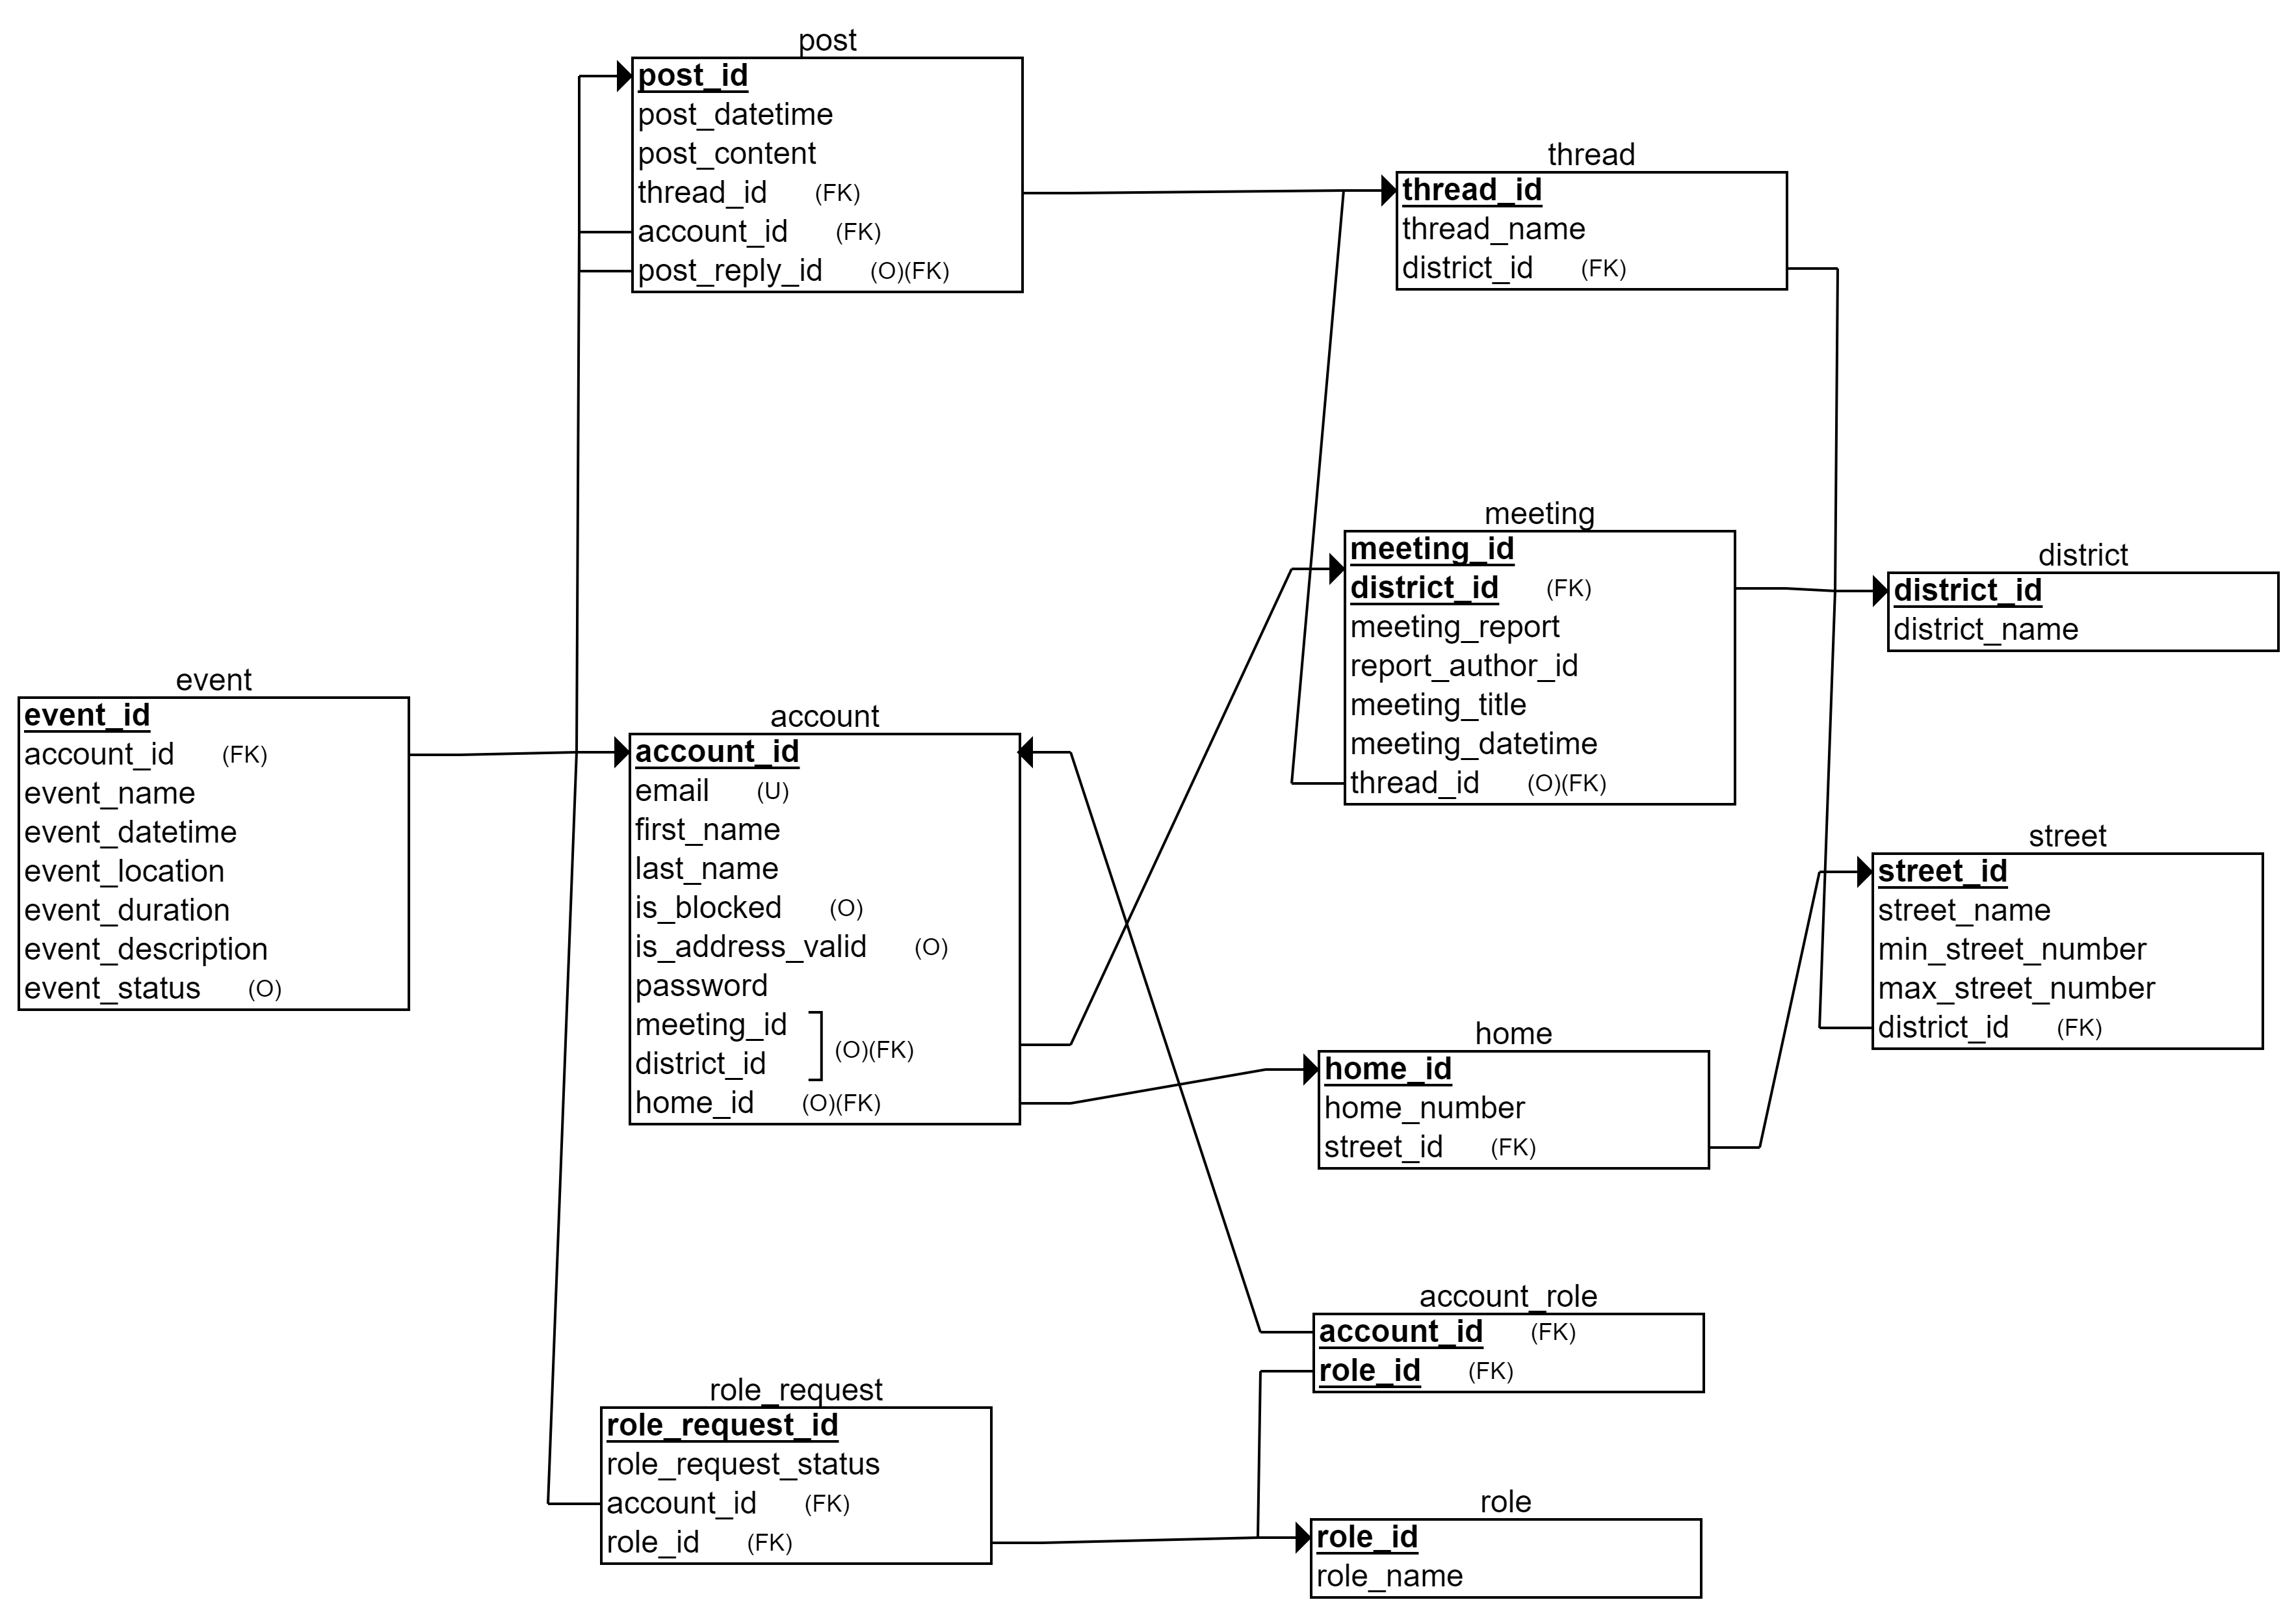
\includegraphics[width = 200mm,scale = 3]{11 relacijska shema baze podataka.png}}
  \caption{Relacijska shema baze podataka}
  \label{Relacijska_shema}
\end{figure}
			
			\eject
			
		\section{Dijagram razreda}
		
		Backend aplikacije je ostvaren korištenjem radnog okvira Spring Boot, i stoga aplikacija ima nekoliko slojeva.
		
		Iako se ne smatraju posebnim slojem, na slici 4.2 prikazani su entiteti koji odgovaraju relacijama u bazi podataka, opisanoj u poglavlju 4.1. Entiteti ne sadrže nikakvu proceduralnu logiku, nego isključivo članske varijable i njihove gettere i settere. Entitetu našoj aplikaciji su redom: Account, District, Event, Home, Meeting, Post, Role, RoleRequest, Street i PostThread.
		
		Na slici 4.3 prikazan je sloj Repository. Razredi u njemu se definiraju kao sučelja koja nude metode dohvaćanja elemenata iz baze, te stvaranja promjena u bazi. Njihov kod u pravilu programer ne piše eksplicitno, nego te metode generira Spring na temelju njihovog imena.
		
		Na slici 4.4 prikazan je sloj Service. Taj sloj sadrži centralnu logiku na backendu, manipulira entitetima i poziva metode koje nudi prethodni sloj, Repository.
		
		Na slici 4.5 prikazan je sloj Controller. Taj je sloj najviši u hijerarhiji slojeva, i on je jedini sloj s kojim komunicira frontend dio aplikacije. Uloga ovog sloja je da obrađuje HTTP zahtjeve, poziva metode koje nudi prethodni sloj Service, i potom odgovara na primljene zahtjeve.
		
		Zbog preglednosti, na jednom dijagramu nije bilo moguće prikazati sve razrede. Umjesto toga, na sljedeći način su prikazani odnosi među slojevima: na slici 4.6 prikazan je odnos između slojeva Controller i Service, na slici 4.7 prikazan je odnos između slojeva Service i Repository, na slici 4.8 prikazan je odnos između sloja Service i entiteta, te je na slici 4.9 prikazan odnos između sloja Repository i entiteta.
		
		\eject
		
				\begin{figure}[H]
					\centering
					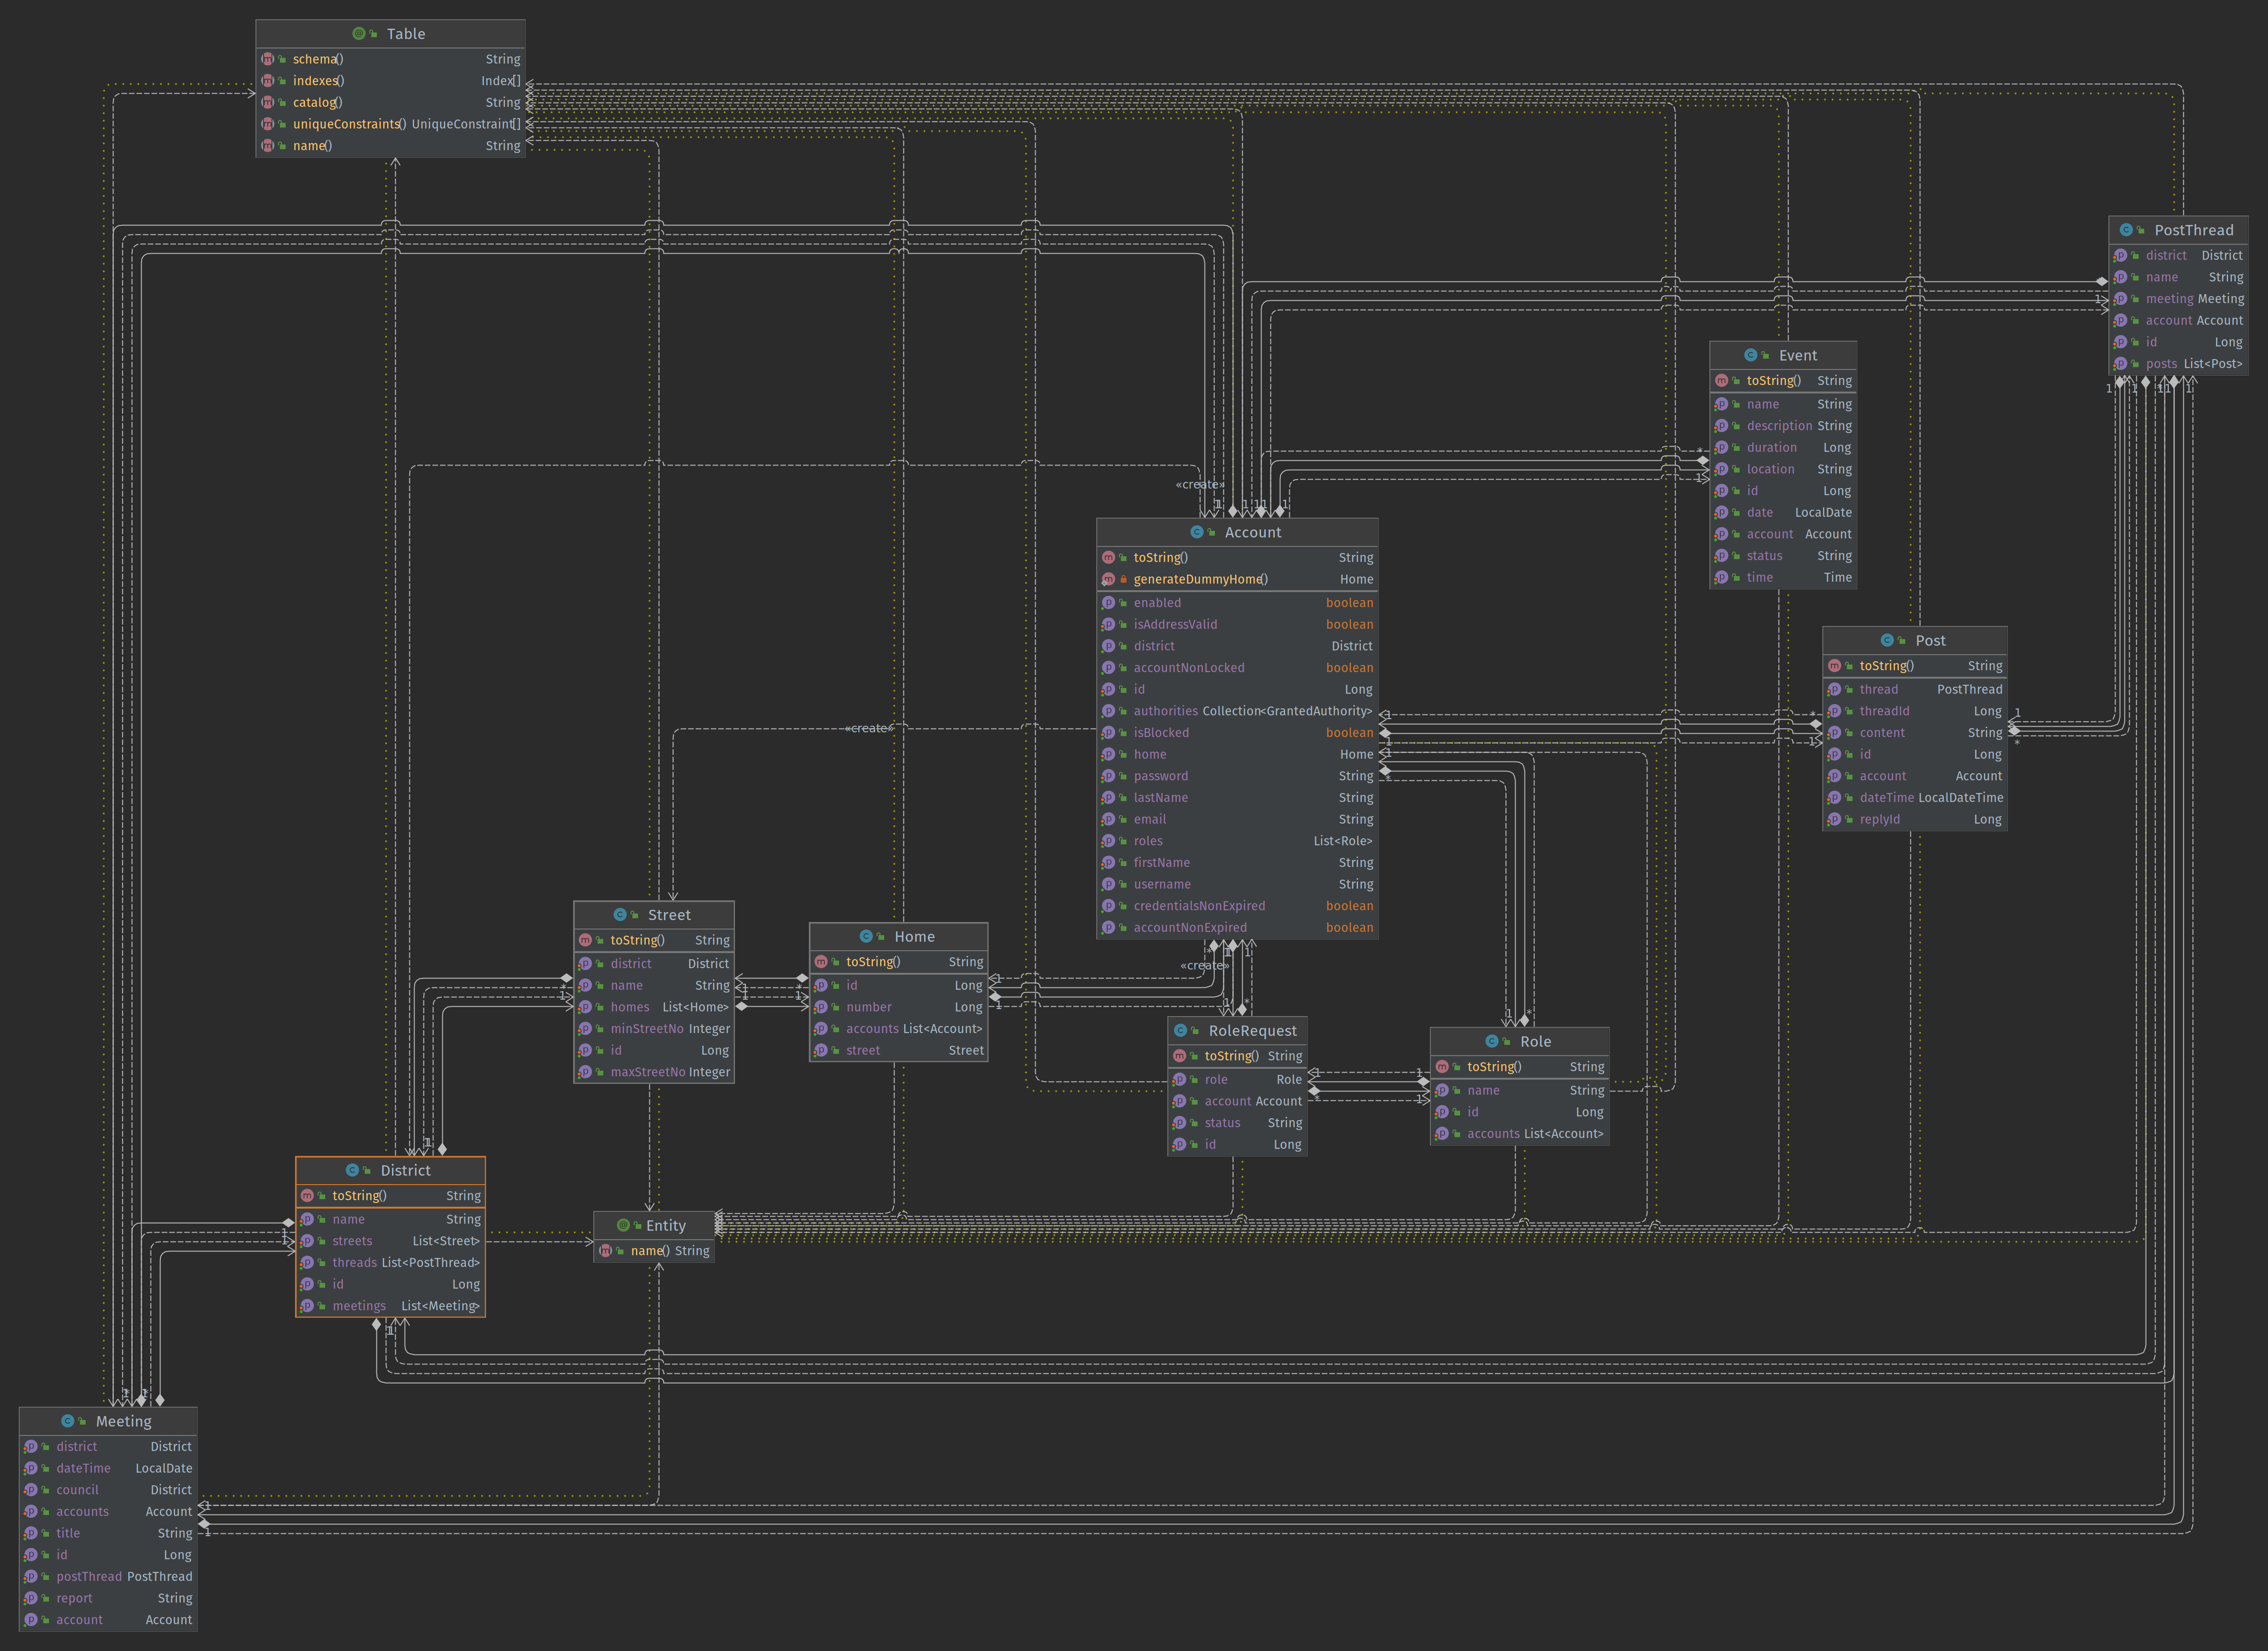
\includegraphics[width=\textwidth,keepaspectratio]{12.1 entiteti.png}
					\caption{Dijagram razreda - entiteti}
				\end{figure}	
				
				\begin{figure}[H]
					\centering
					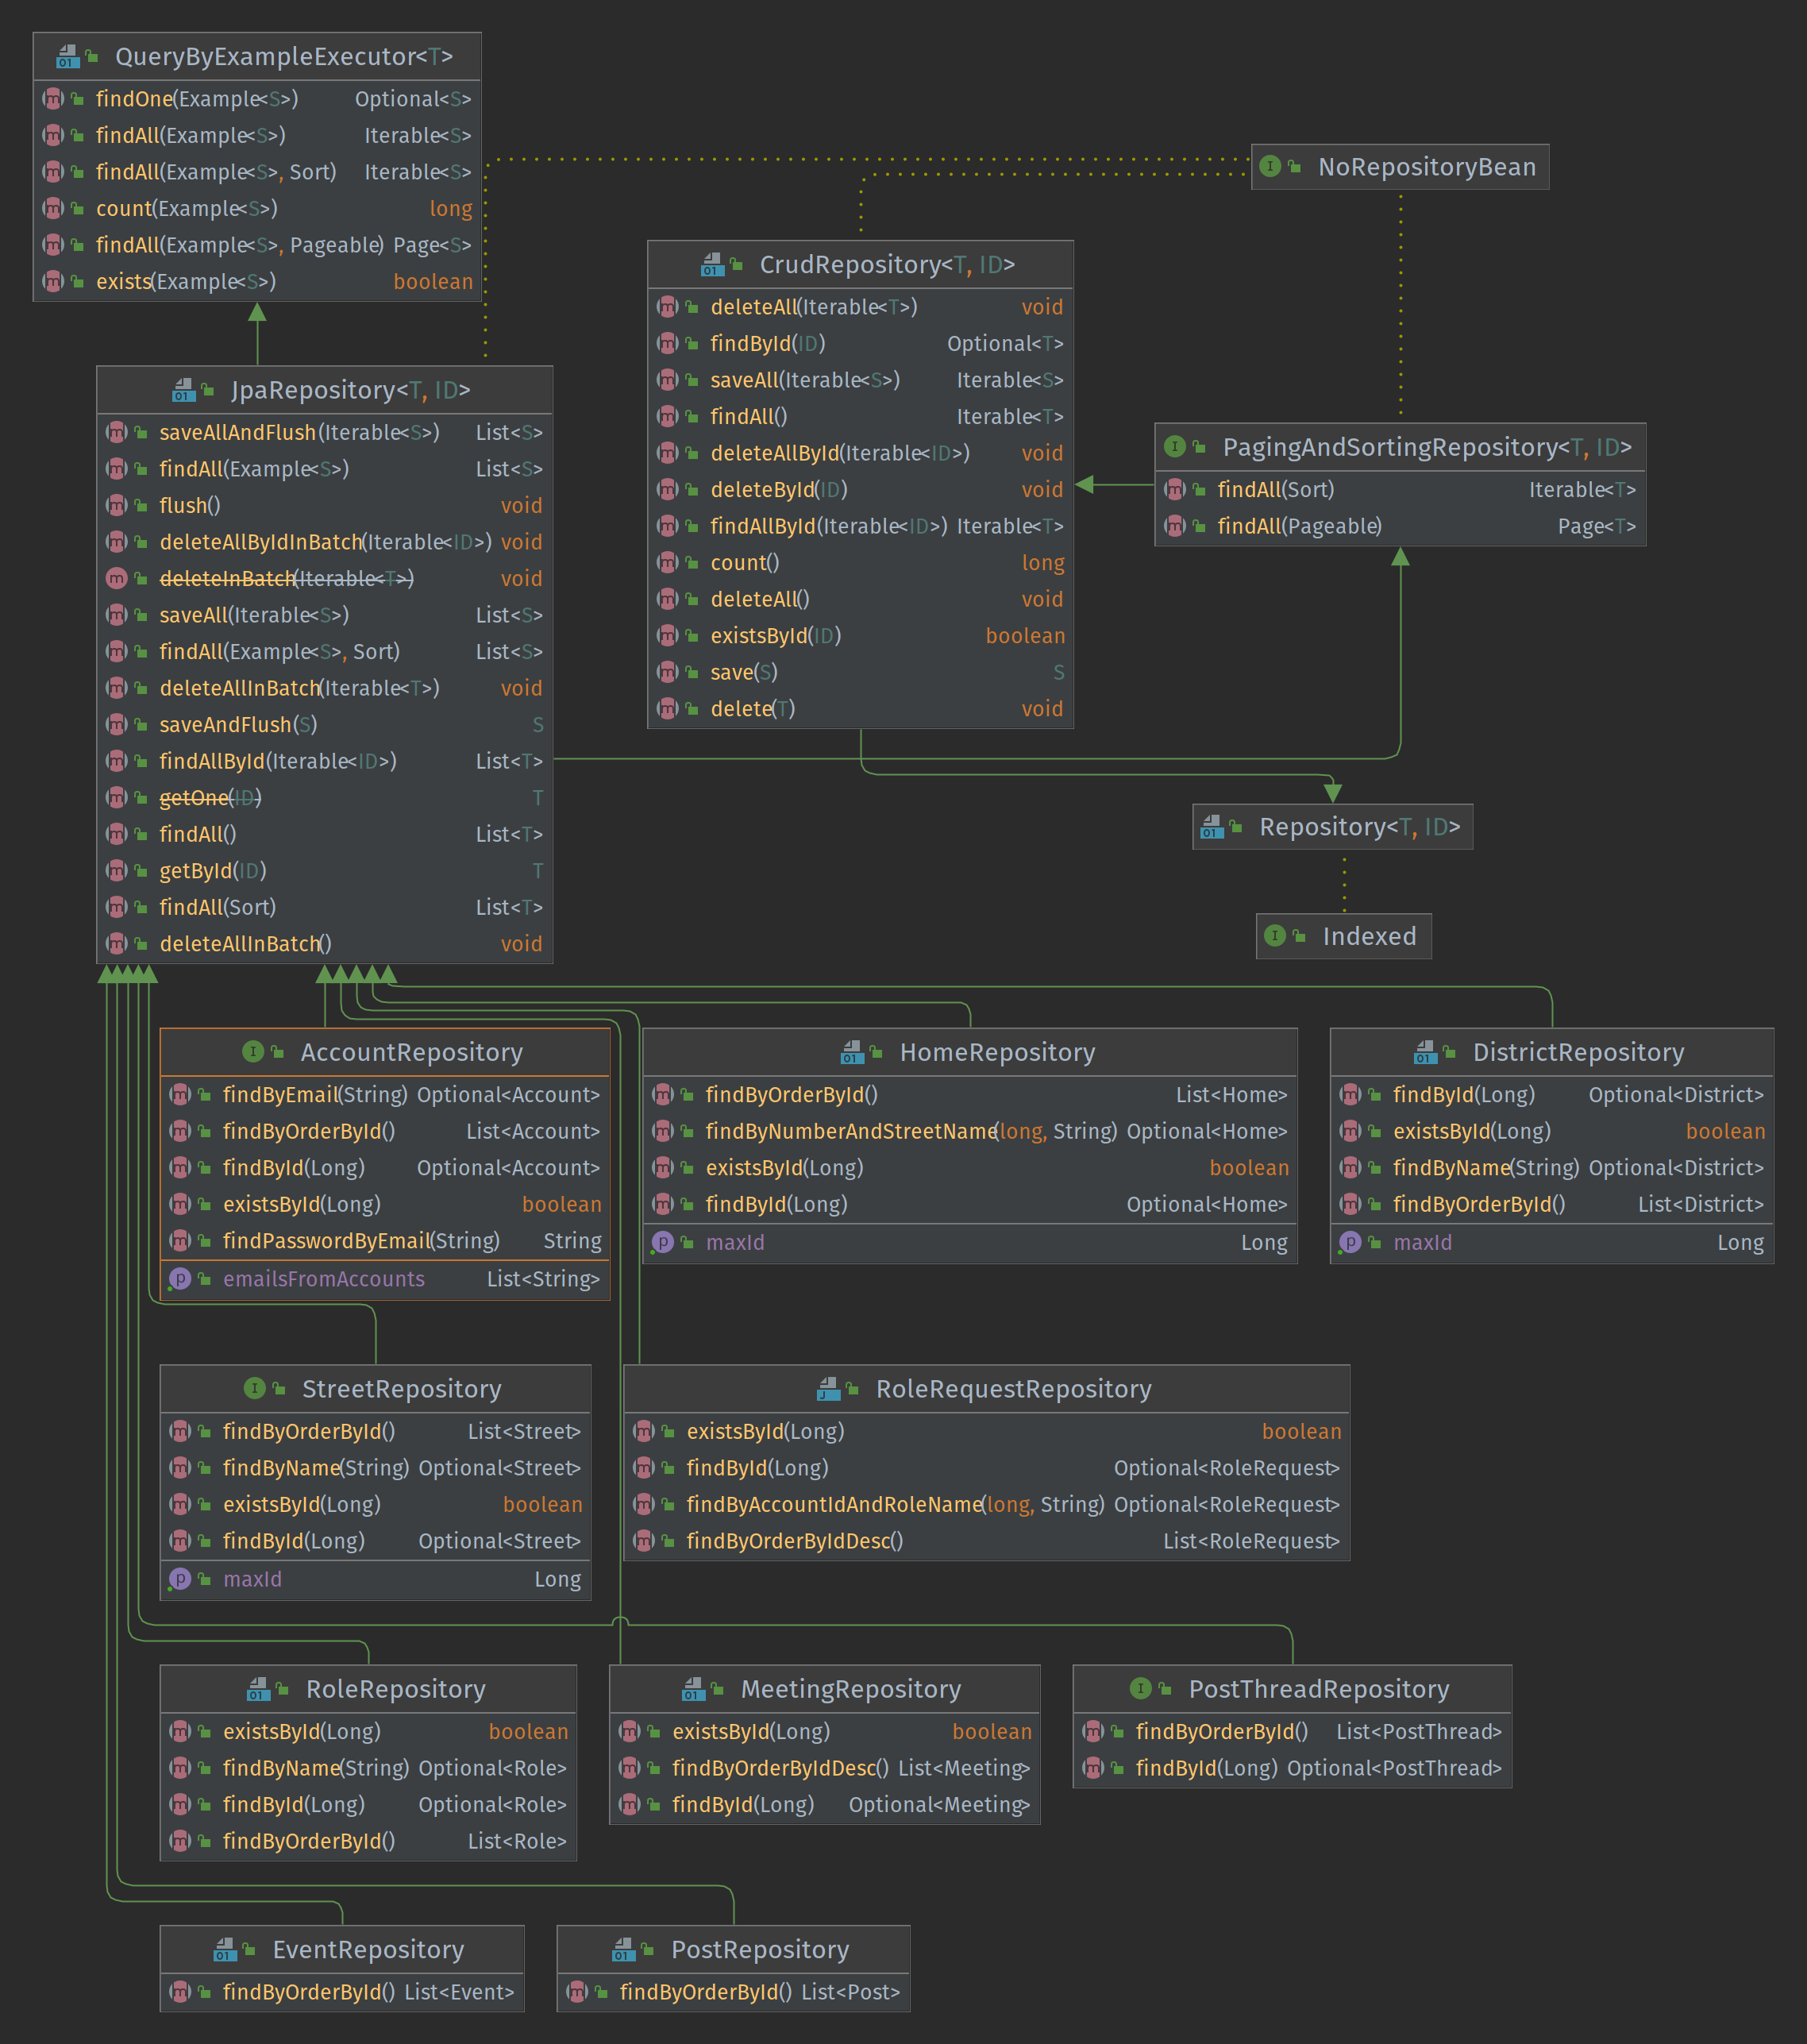
\includegraphics[width=\textwidth,keepaspectratio]{12.2 repozitoriji.png}
					\caption{Dijagram razreda - sloj Repository}
				\end{figure}	
				
				\begin{figure}[H]
					\centering
					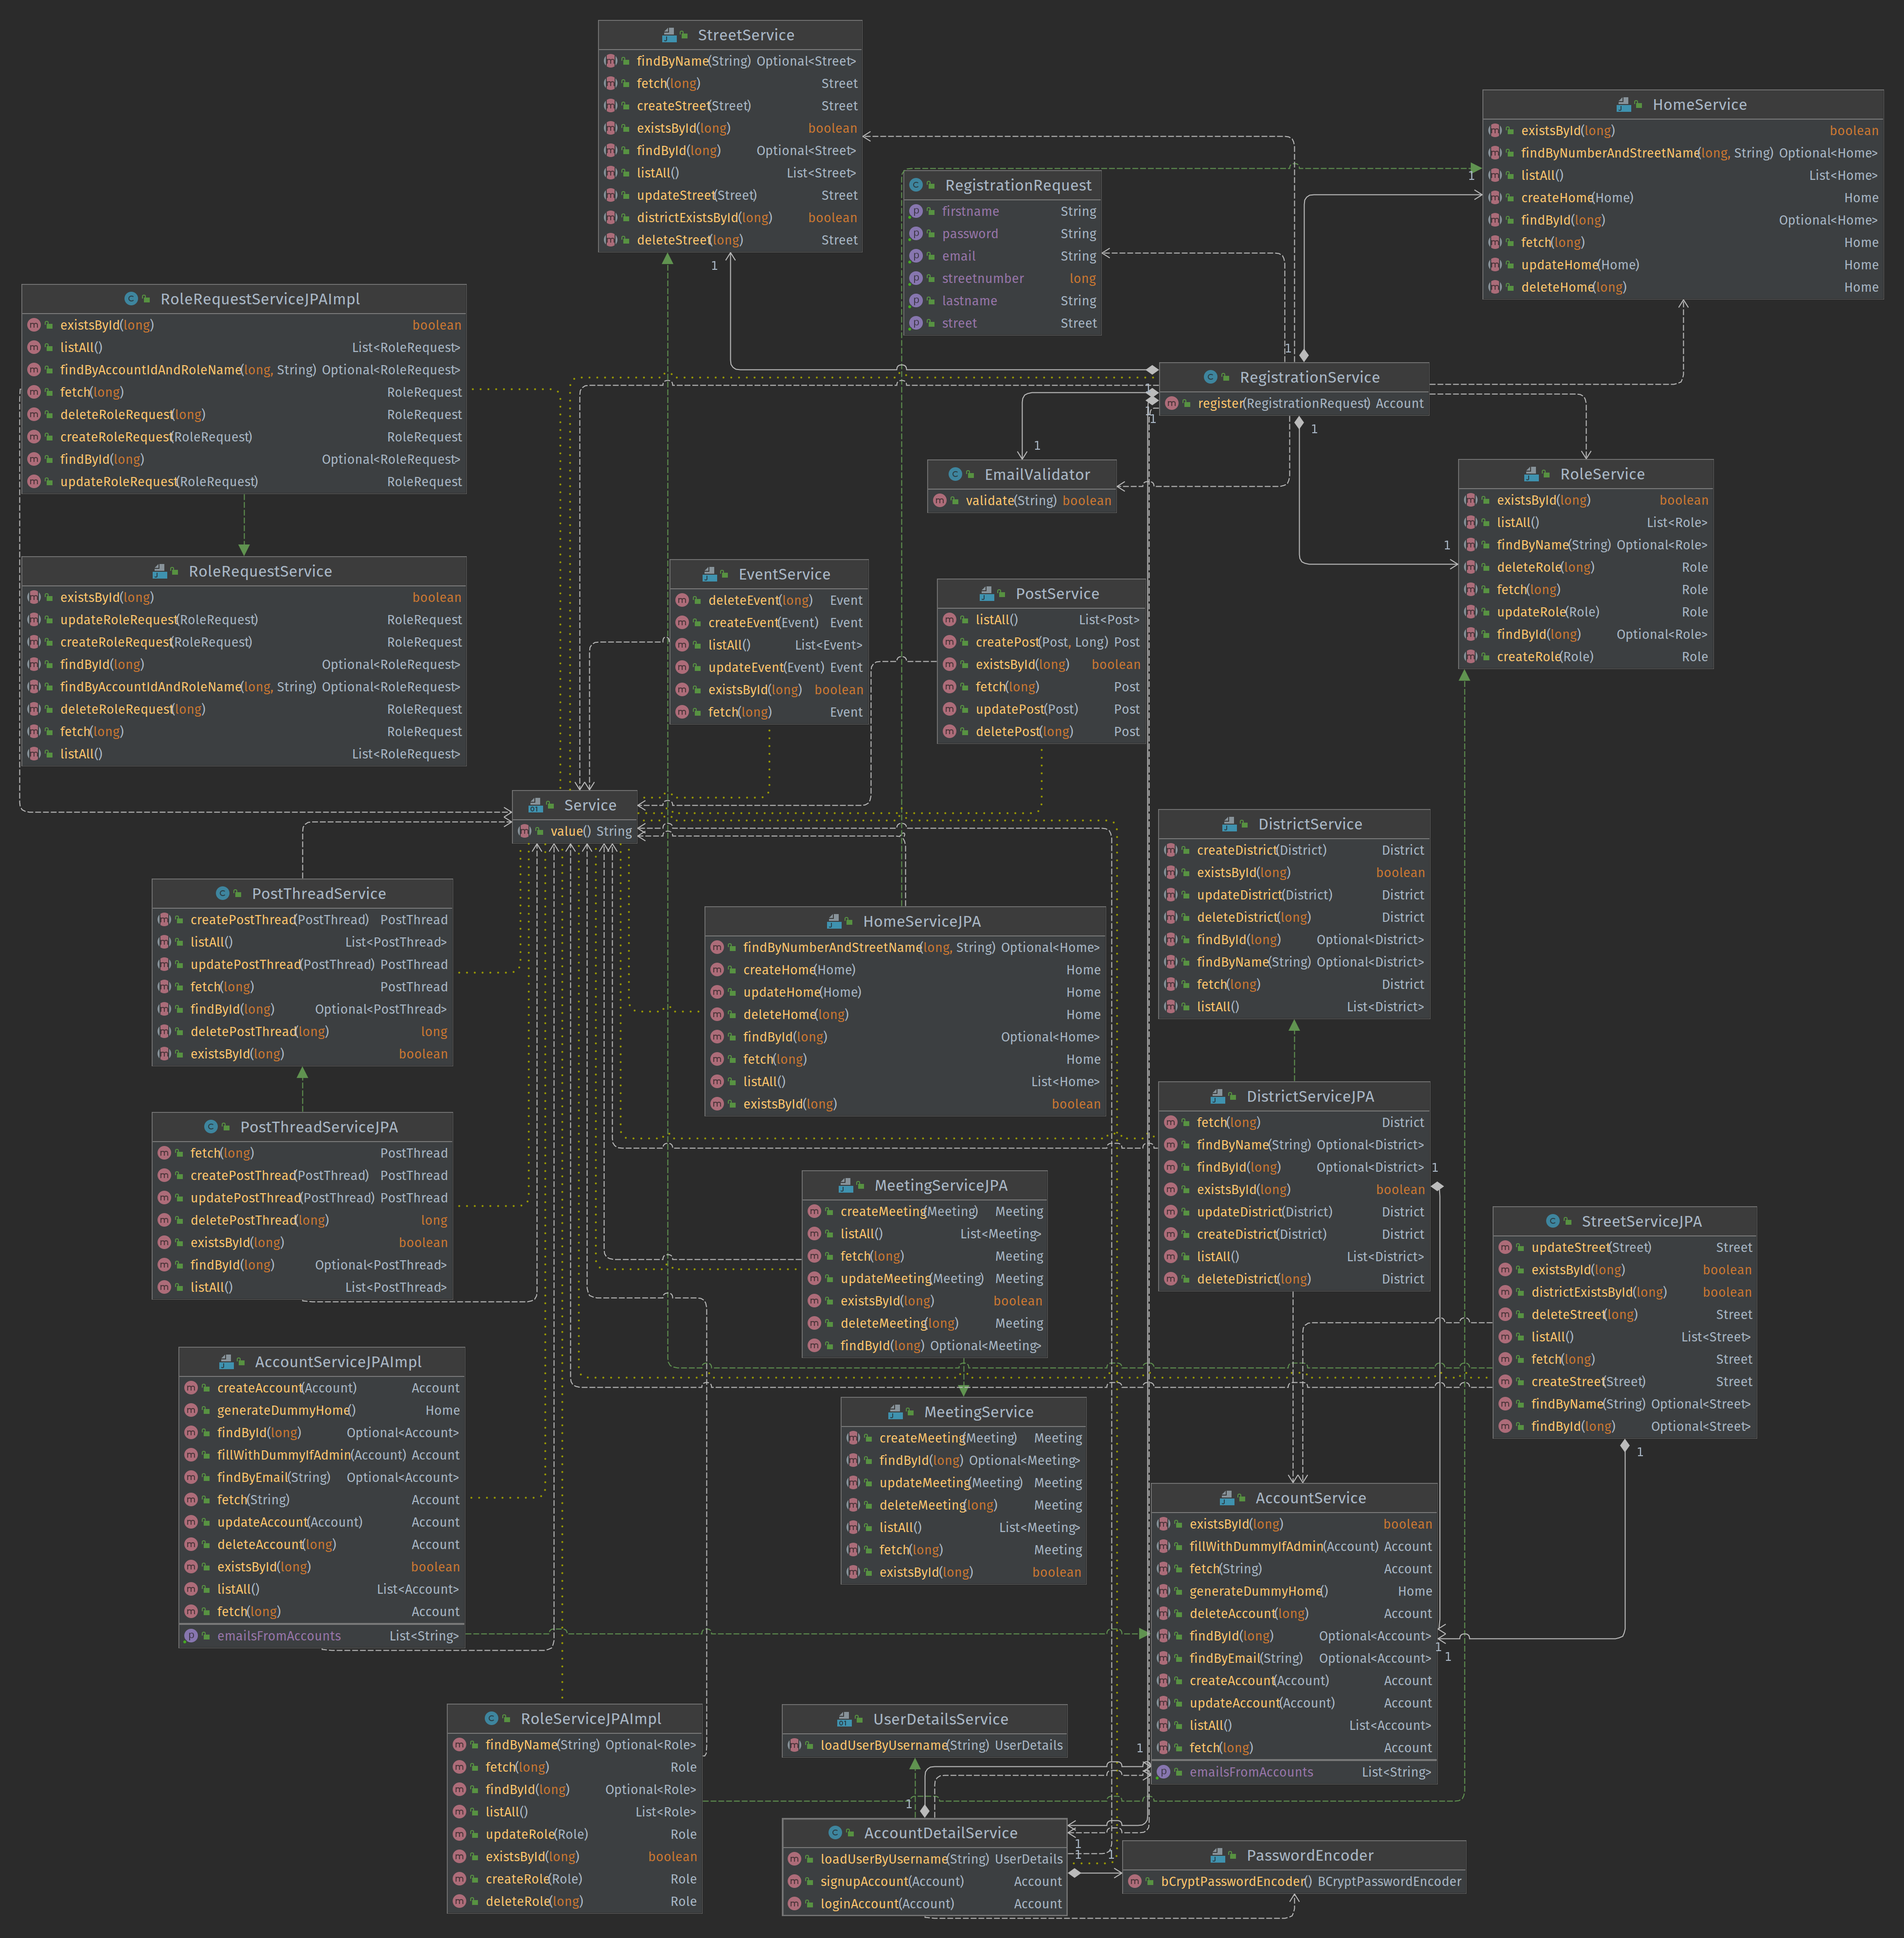
\includegraphics[width=\textwidth,keepaspectratio]{12.3 servisi.png}
					\caption{Dijagram razreda - sloj Service}
				\end{figure}	
				
				\begin{figure}[H]
					\centering
					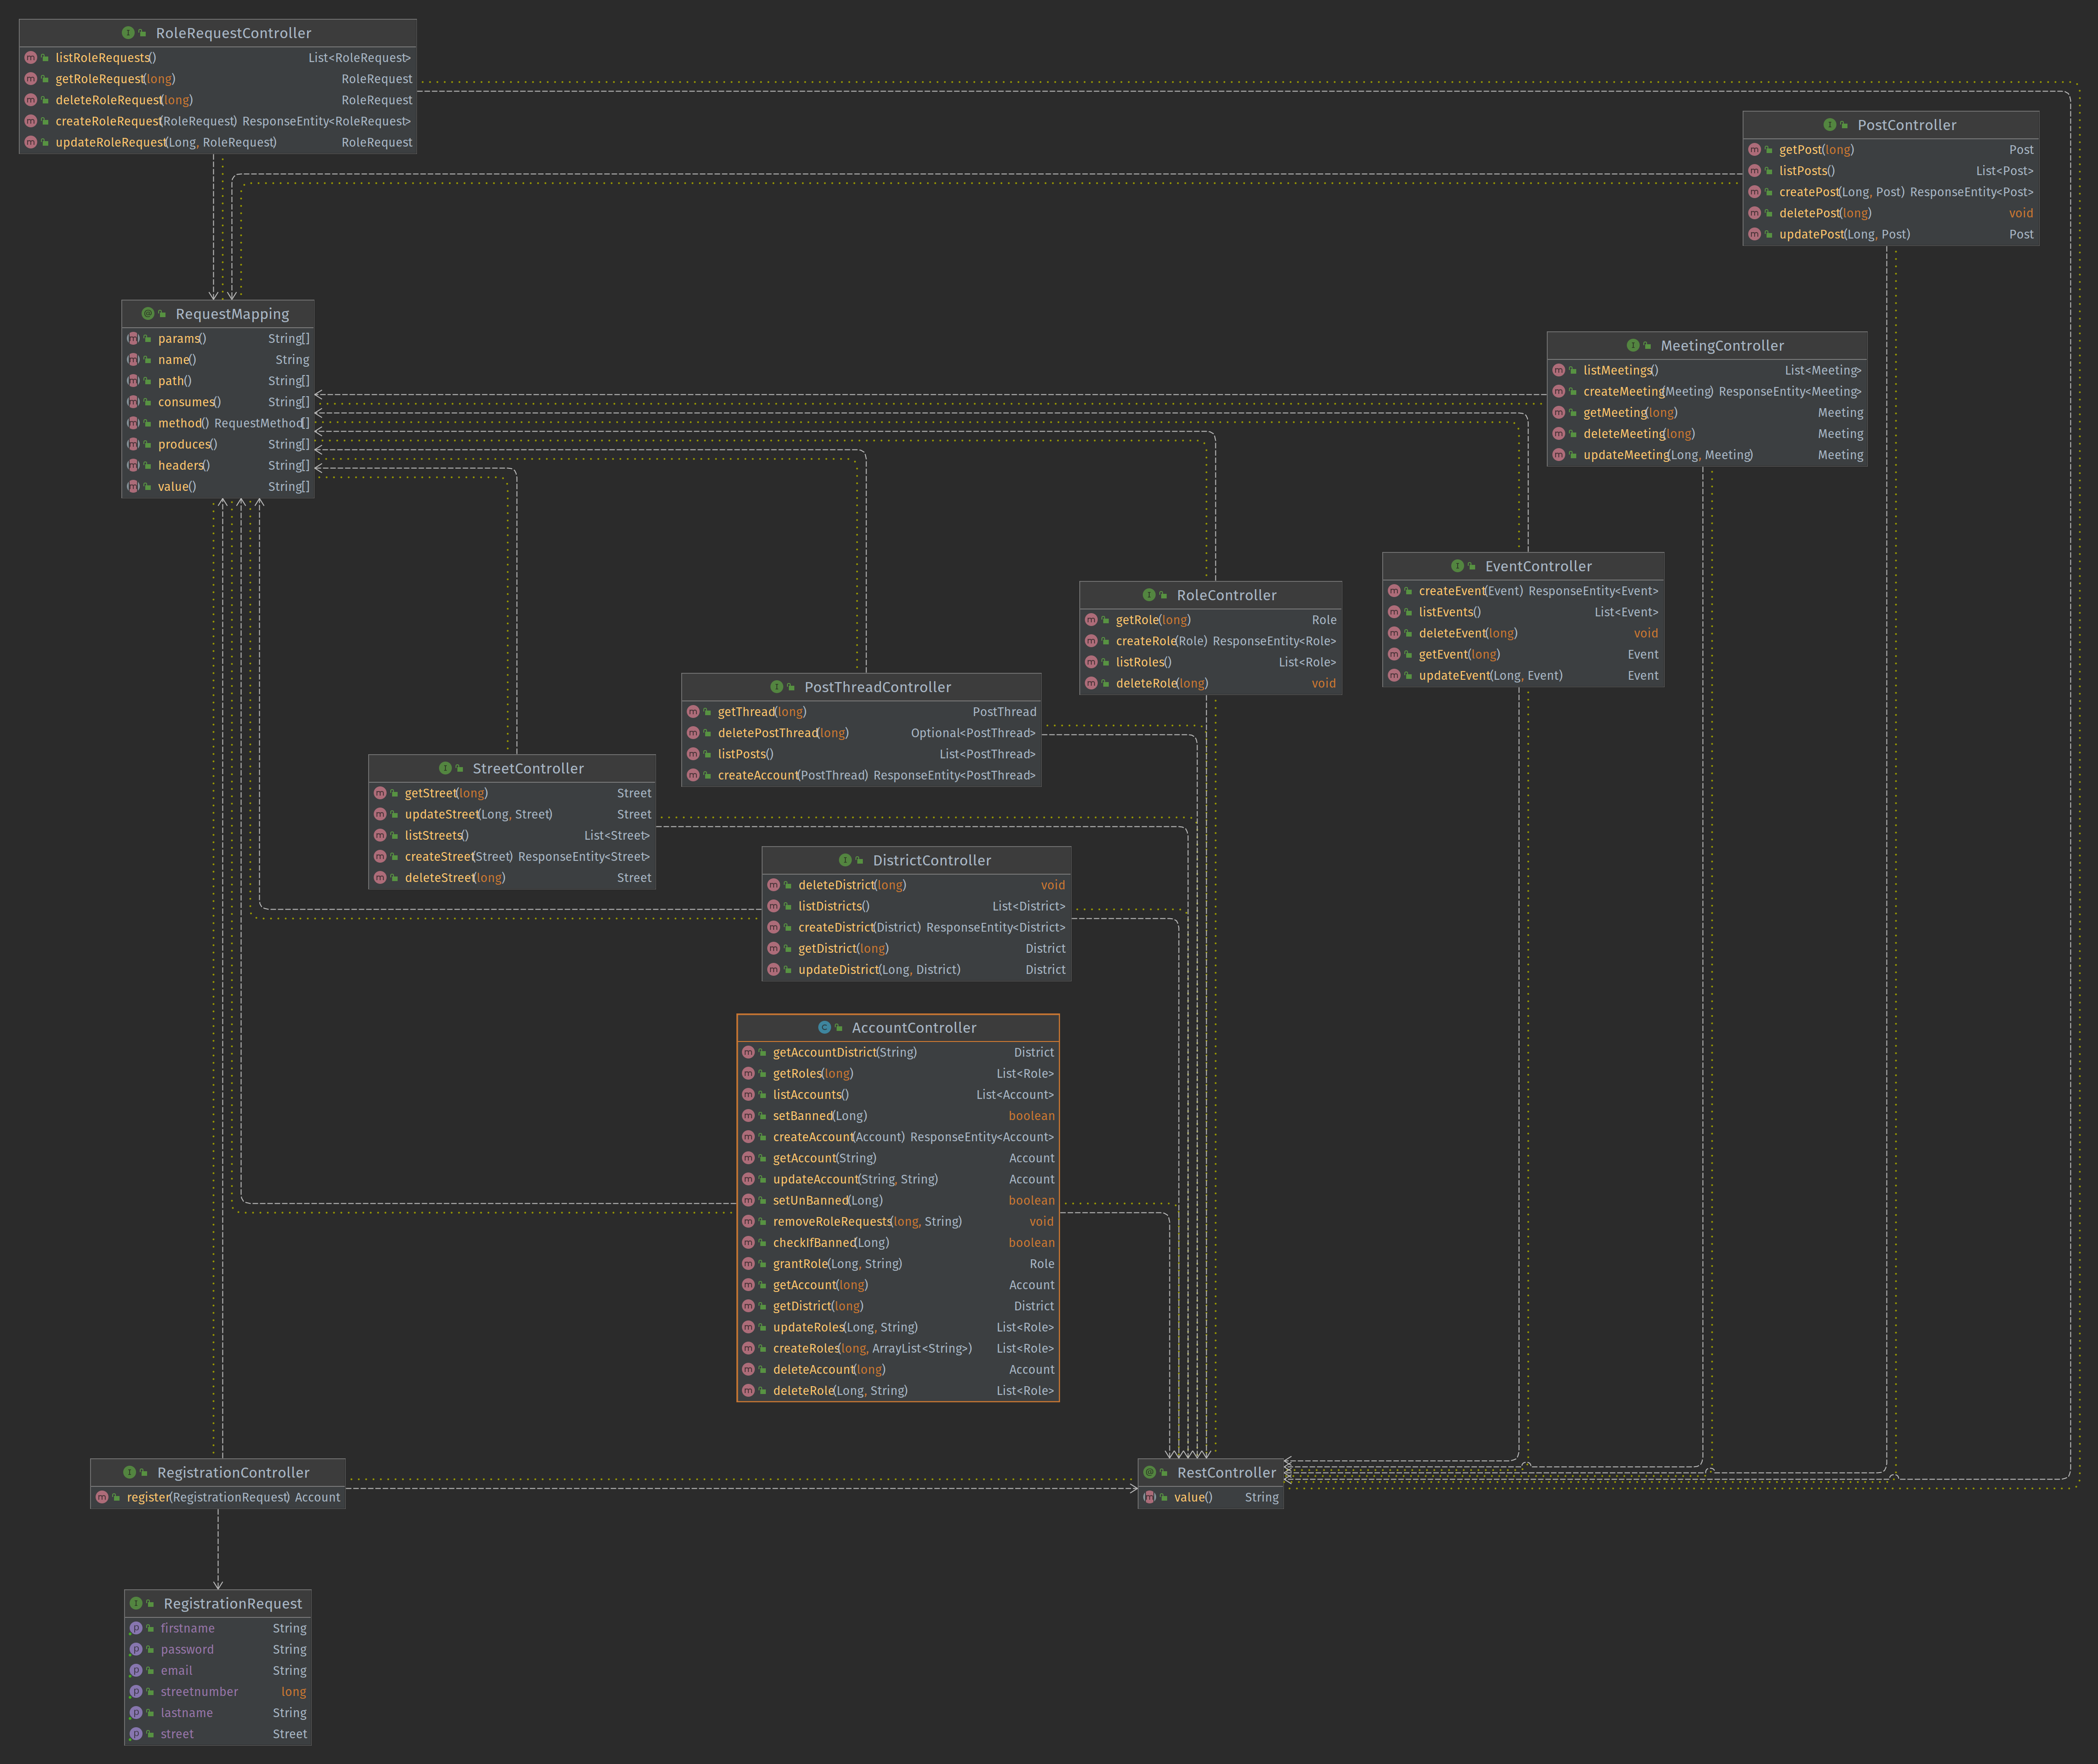
\includegraphics[width=\textwidth,keepaspectratio]{12.4 kontroleri.png}
					\caption{Dijagram razreda - sloj Controller}
				\end{figure}	
				
				\begin{figure}[H]
					\centering
					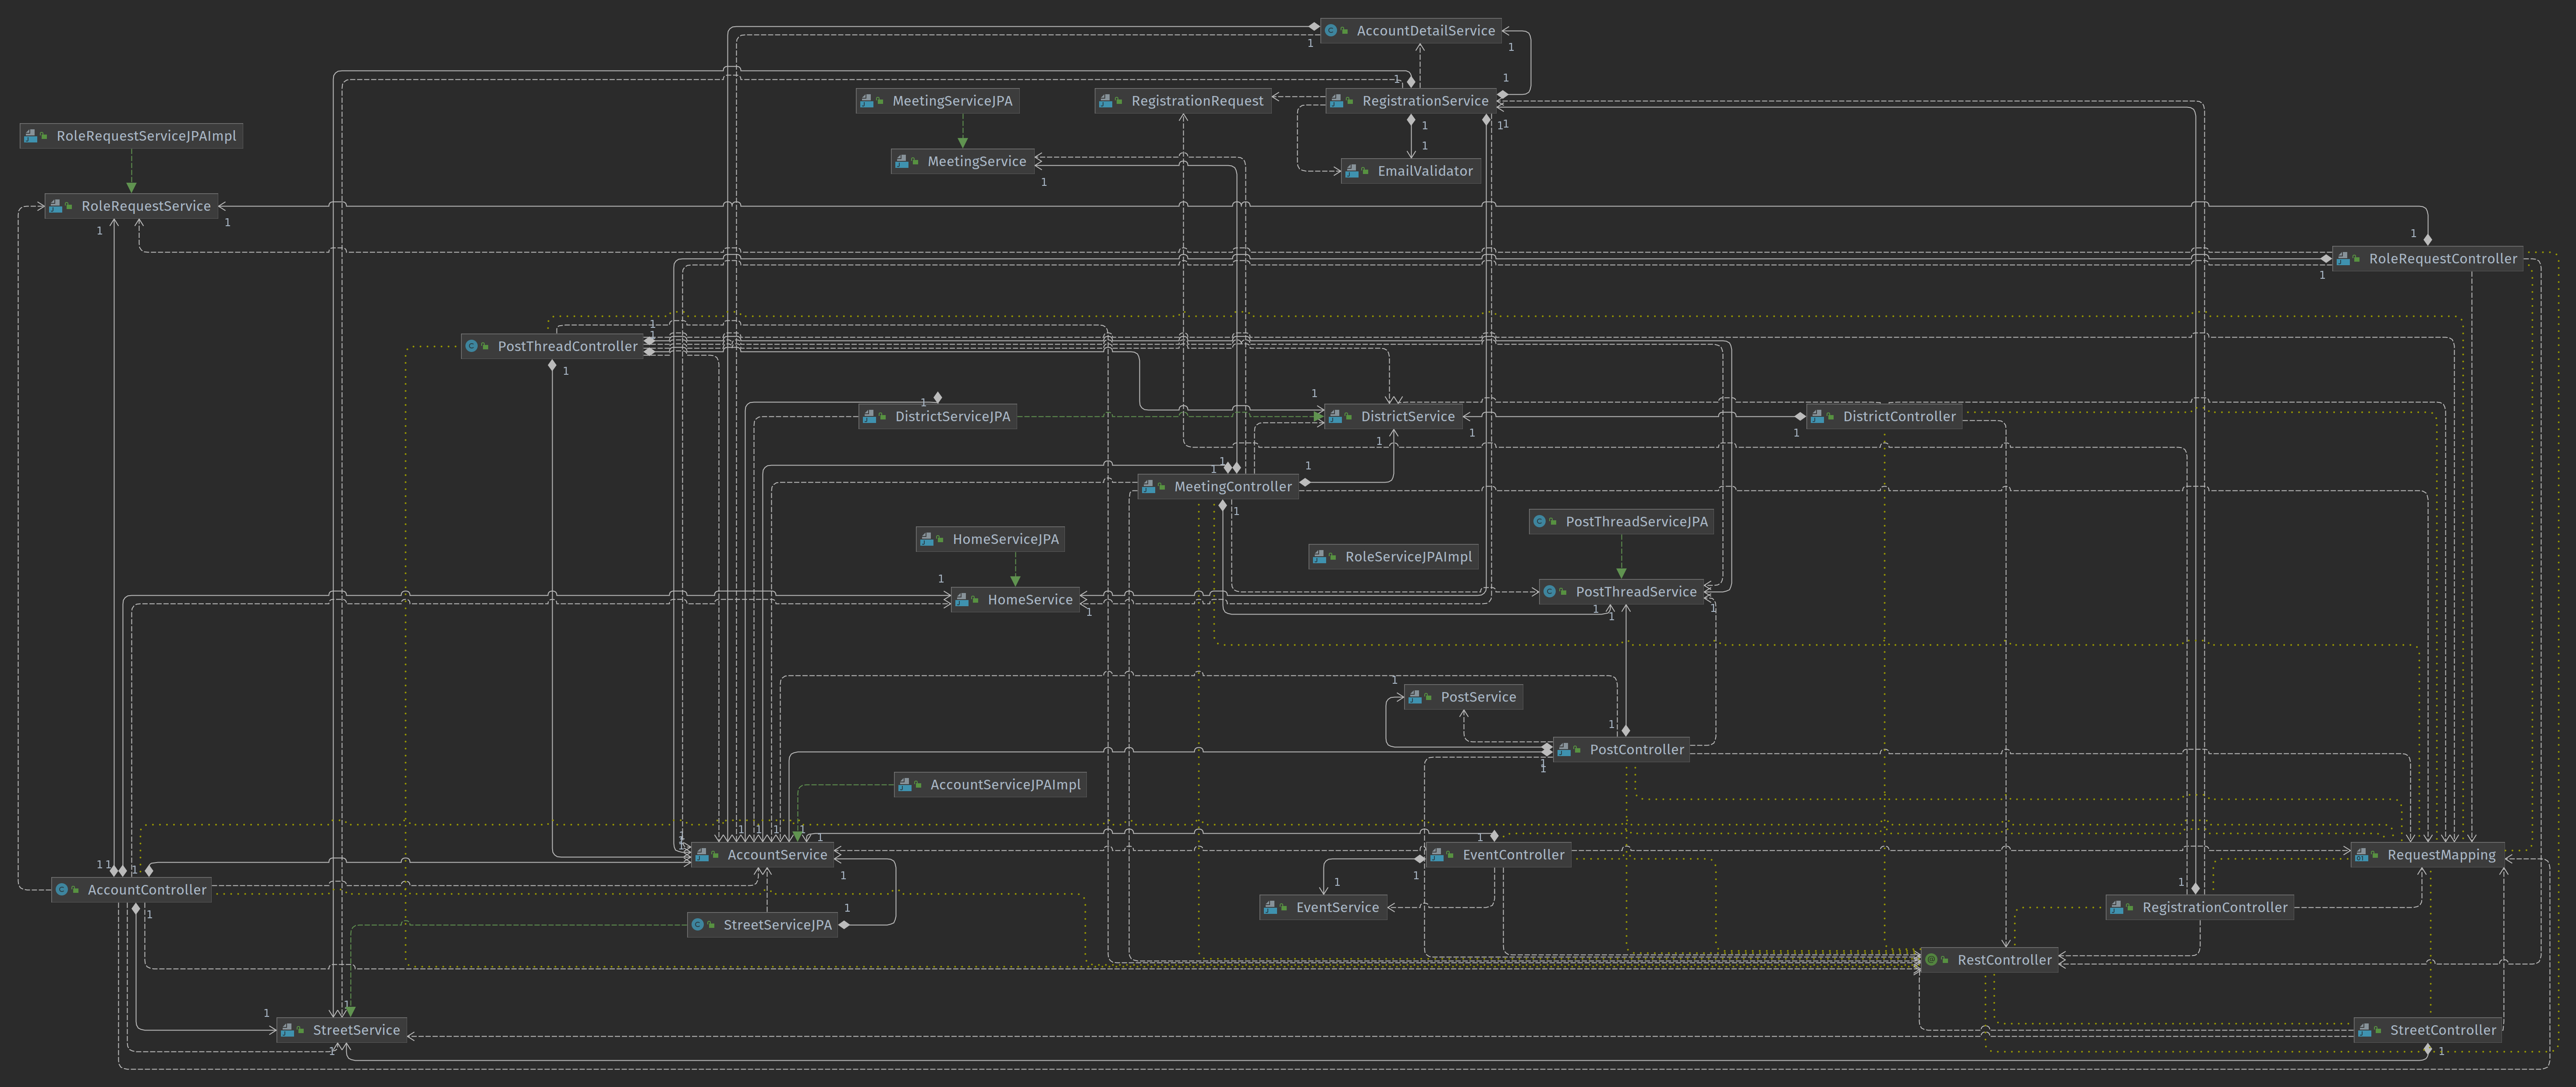
\includegraphics[width=\textwidth,keepaspectratio]{13.1 kontroleri i servisi.png}
					\caption{Dijagram razreda - odnos slojeva Controller i Service}
				\end{figure}	
				
				\begin{figure}[H]
					\centering
					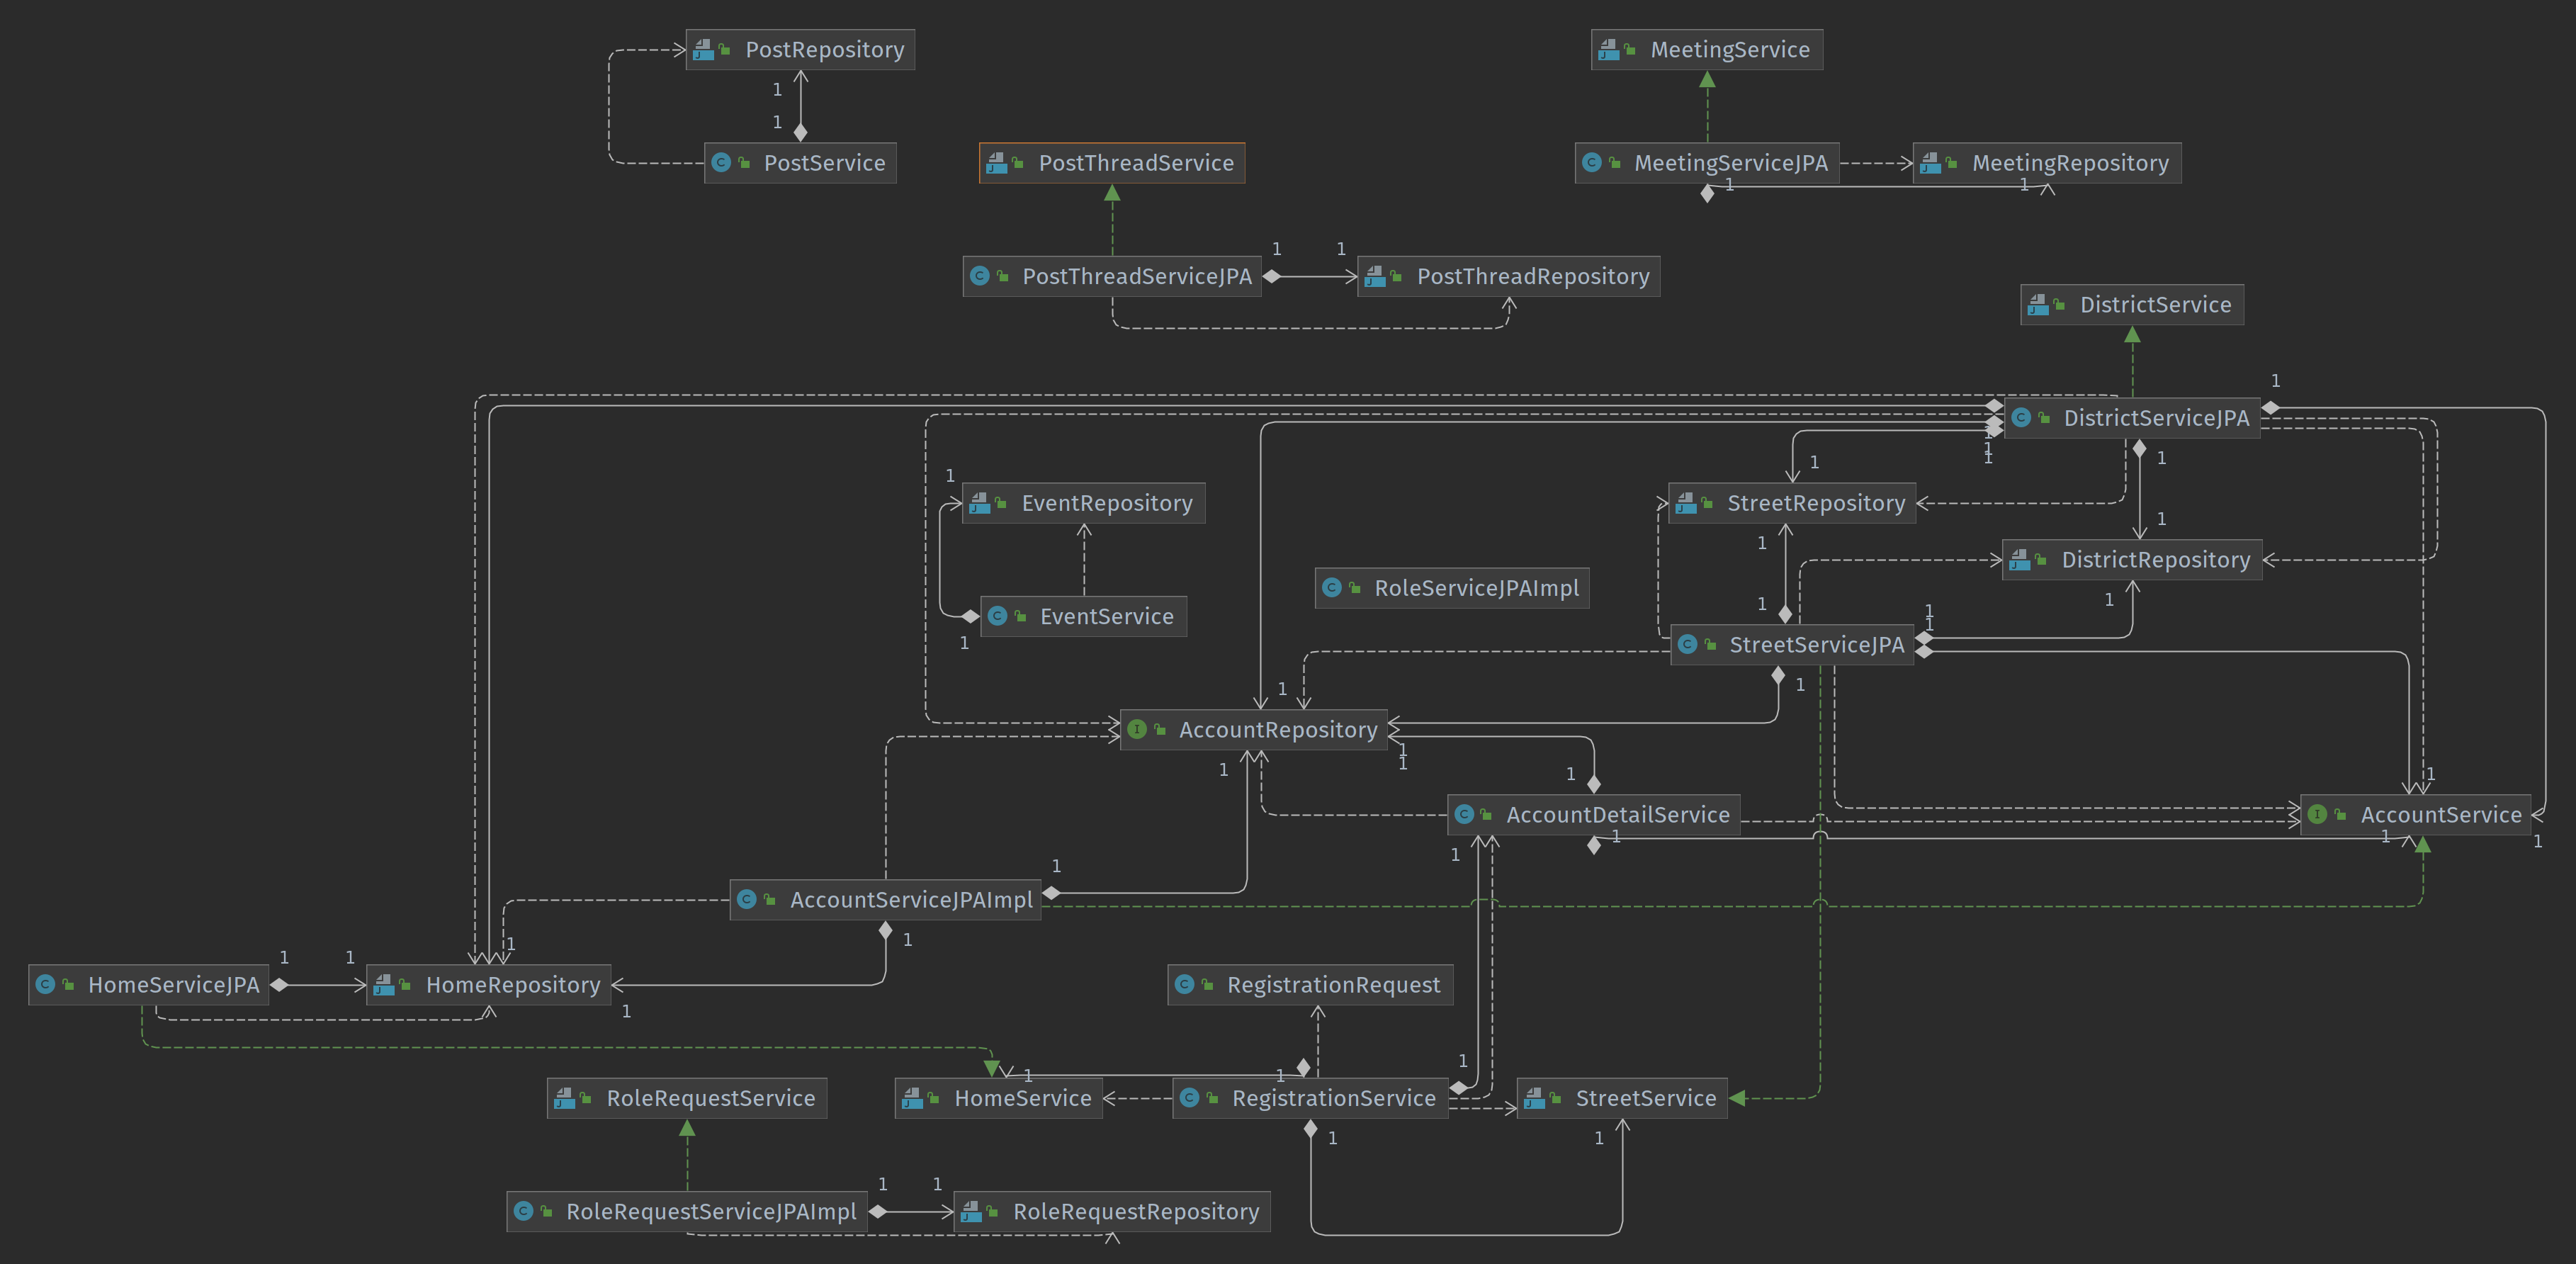
\includegraphics[width=\textwidth,keepaspectratio]{13.2 servisi i repozitoriji.png}
					\caption{Dijagram razreda - odnos slojeva Service i Repository}
				\end{figure}	
				
				\begin{figure}[H]
					\centering
					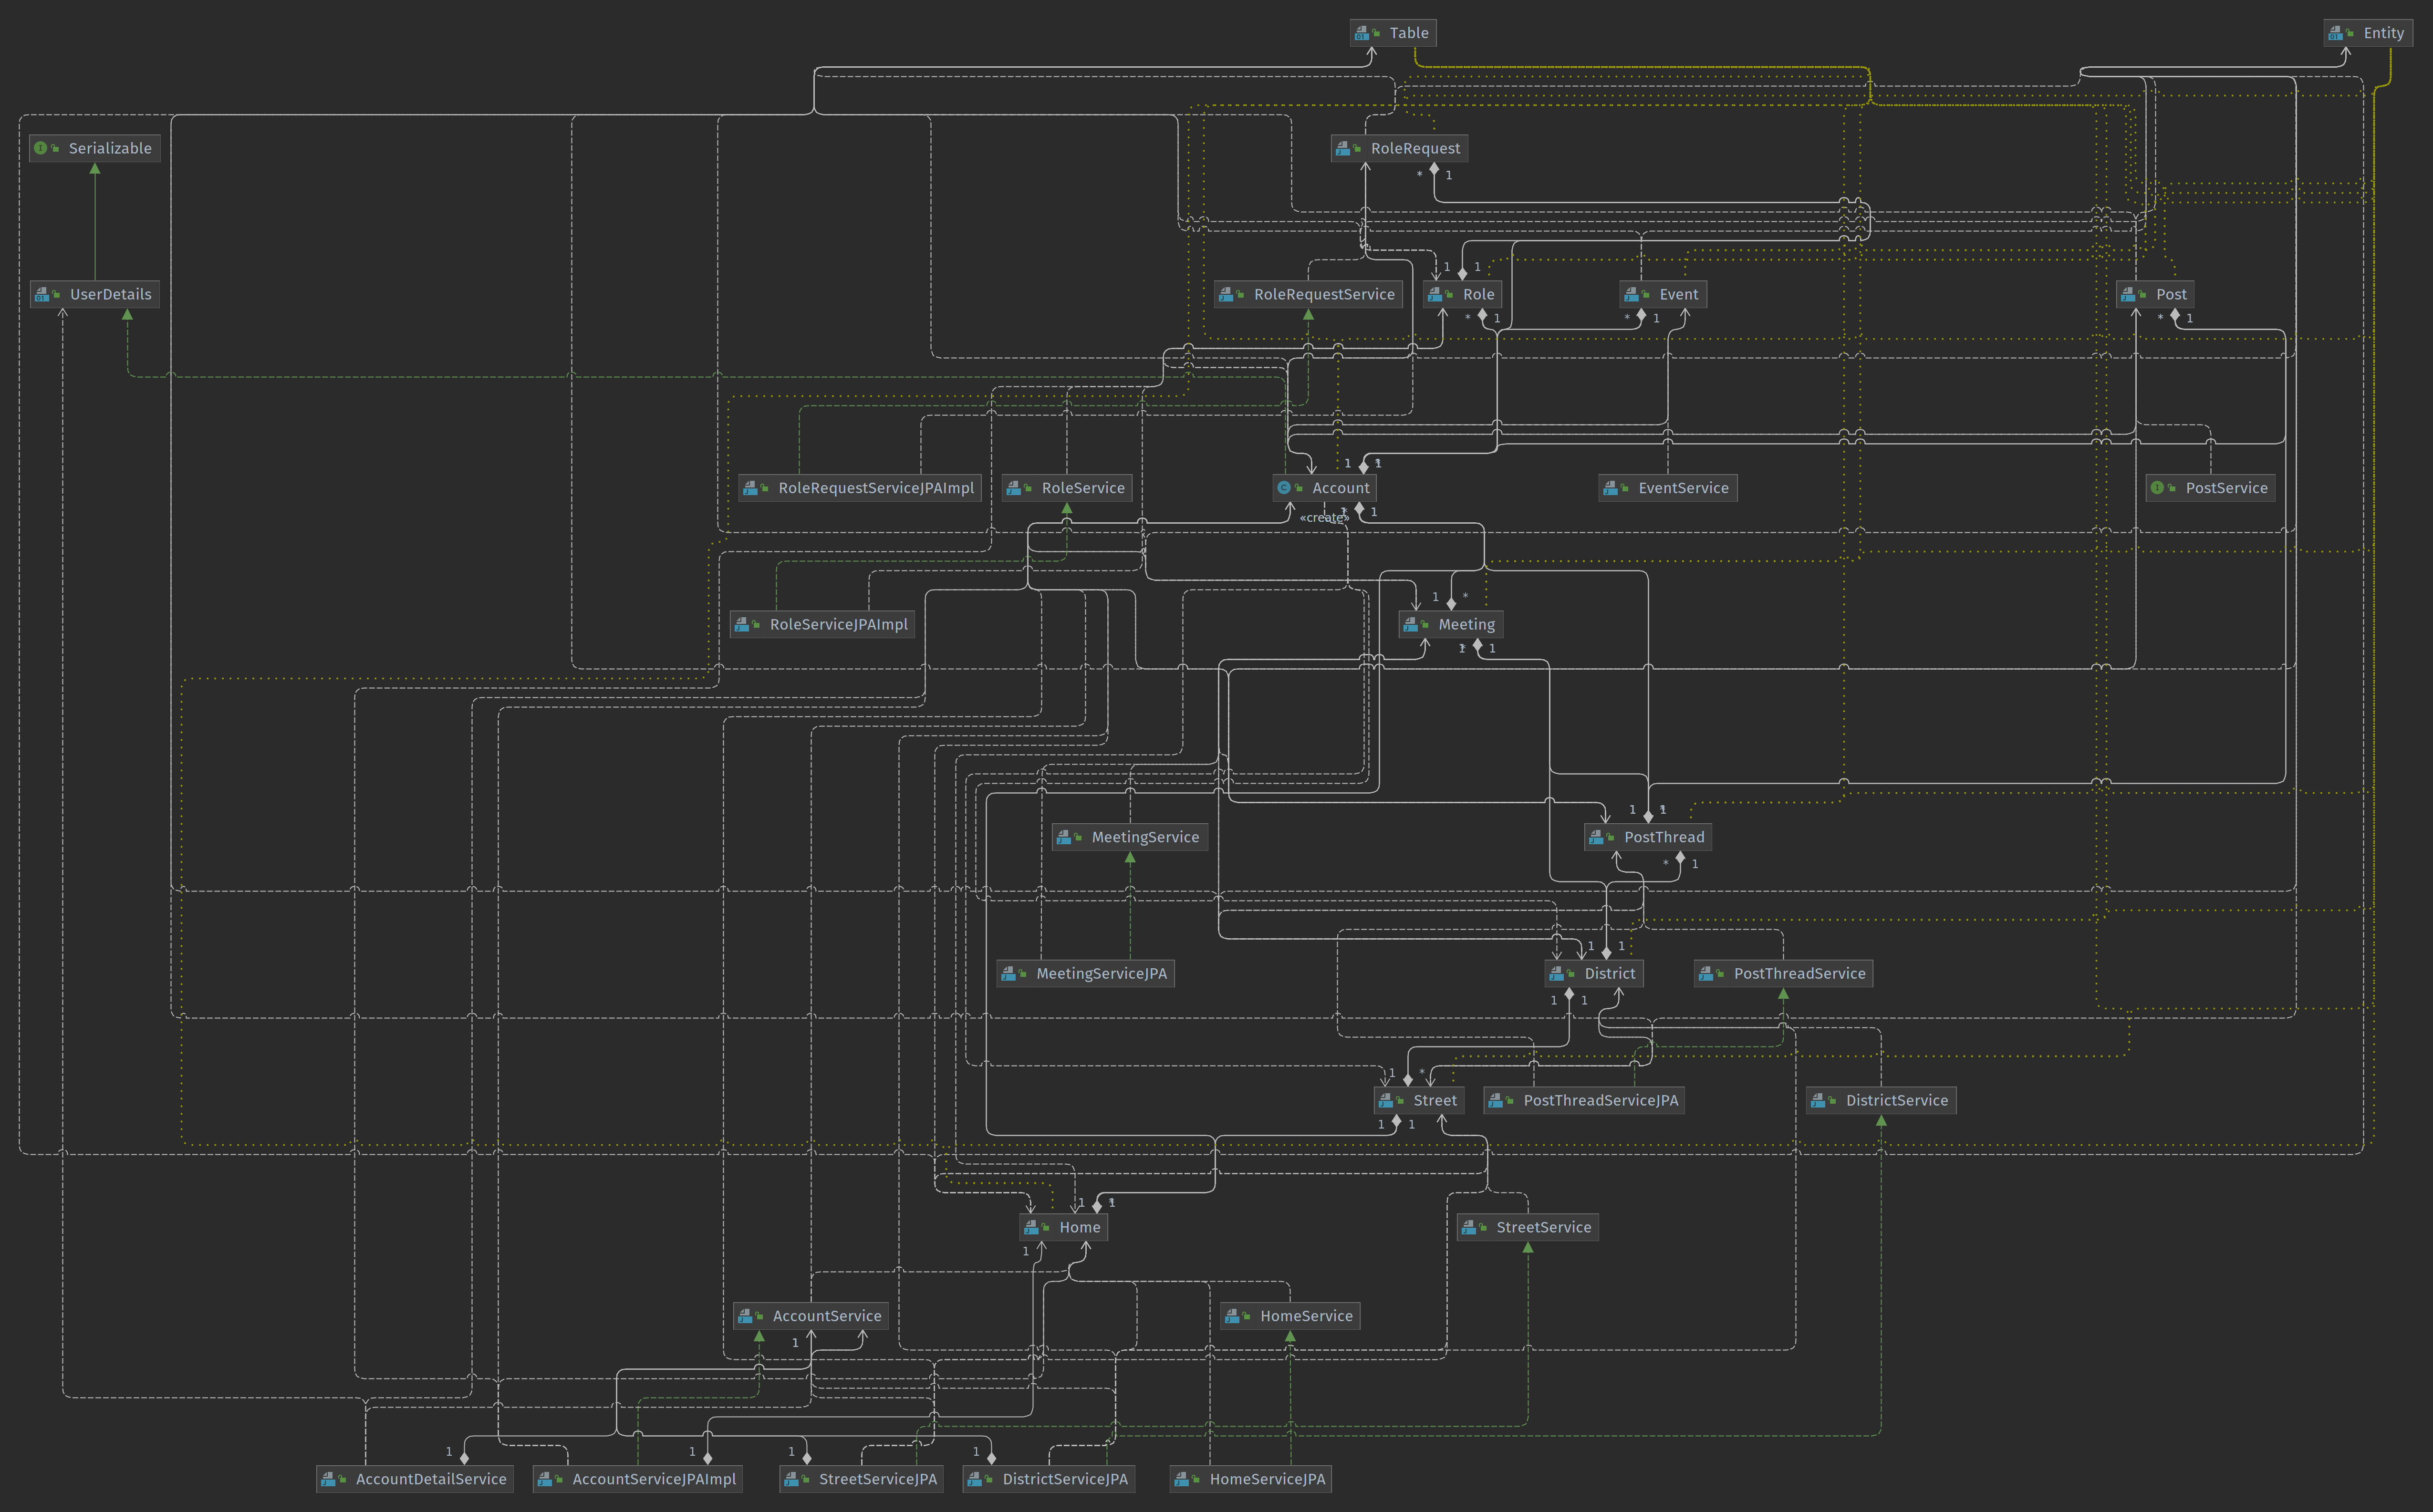
\includegraphics[width=\textwidth,keepaspectratio]{13.3 servisi i entiteti.png}
					\caption{Dijagram razreda - odnos sloja Service i entiteta}
				\end{figure}	
				
				\begin{figure}[H]
					\centering
					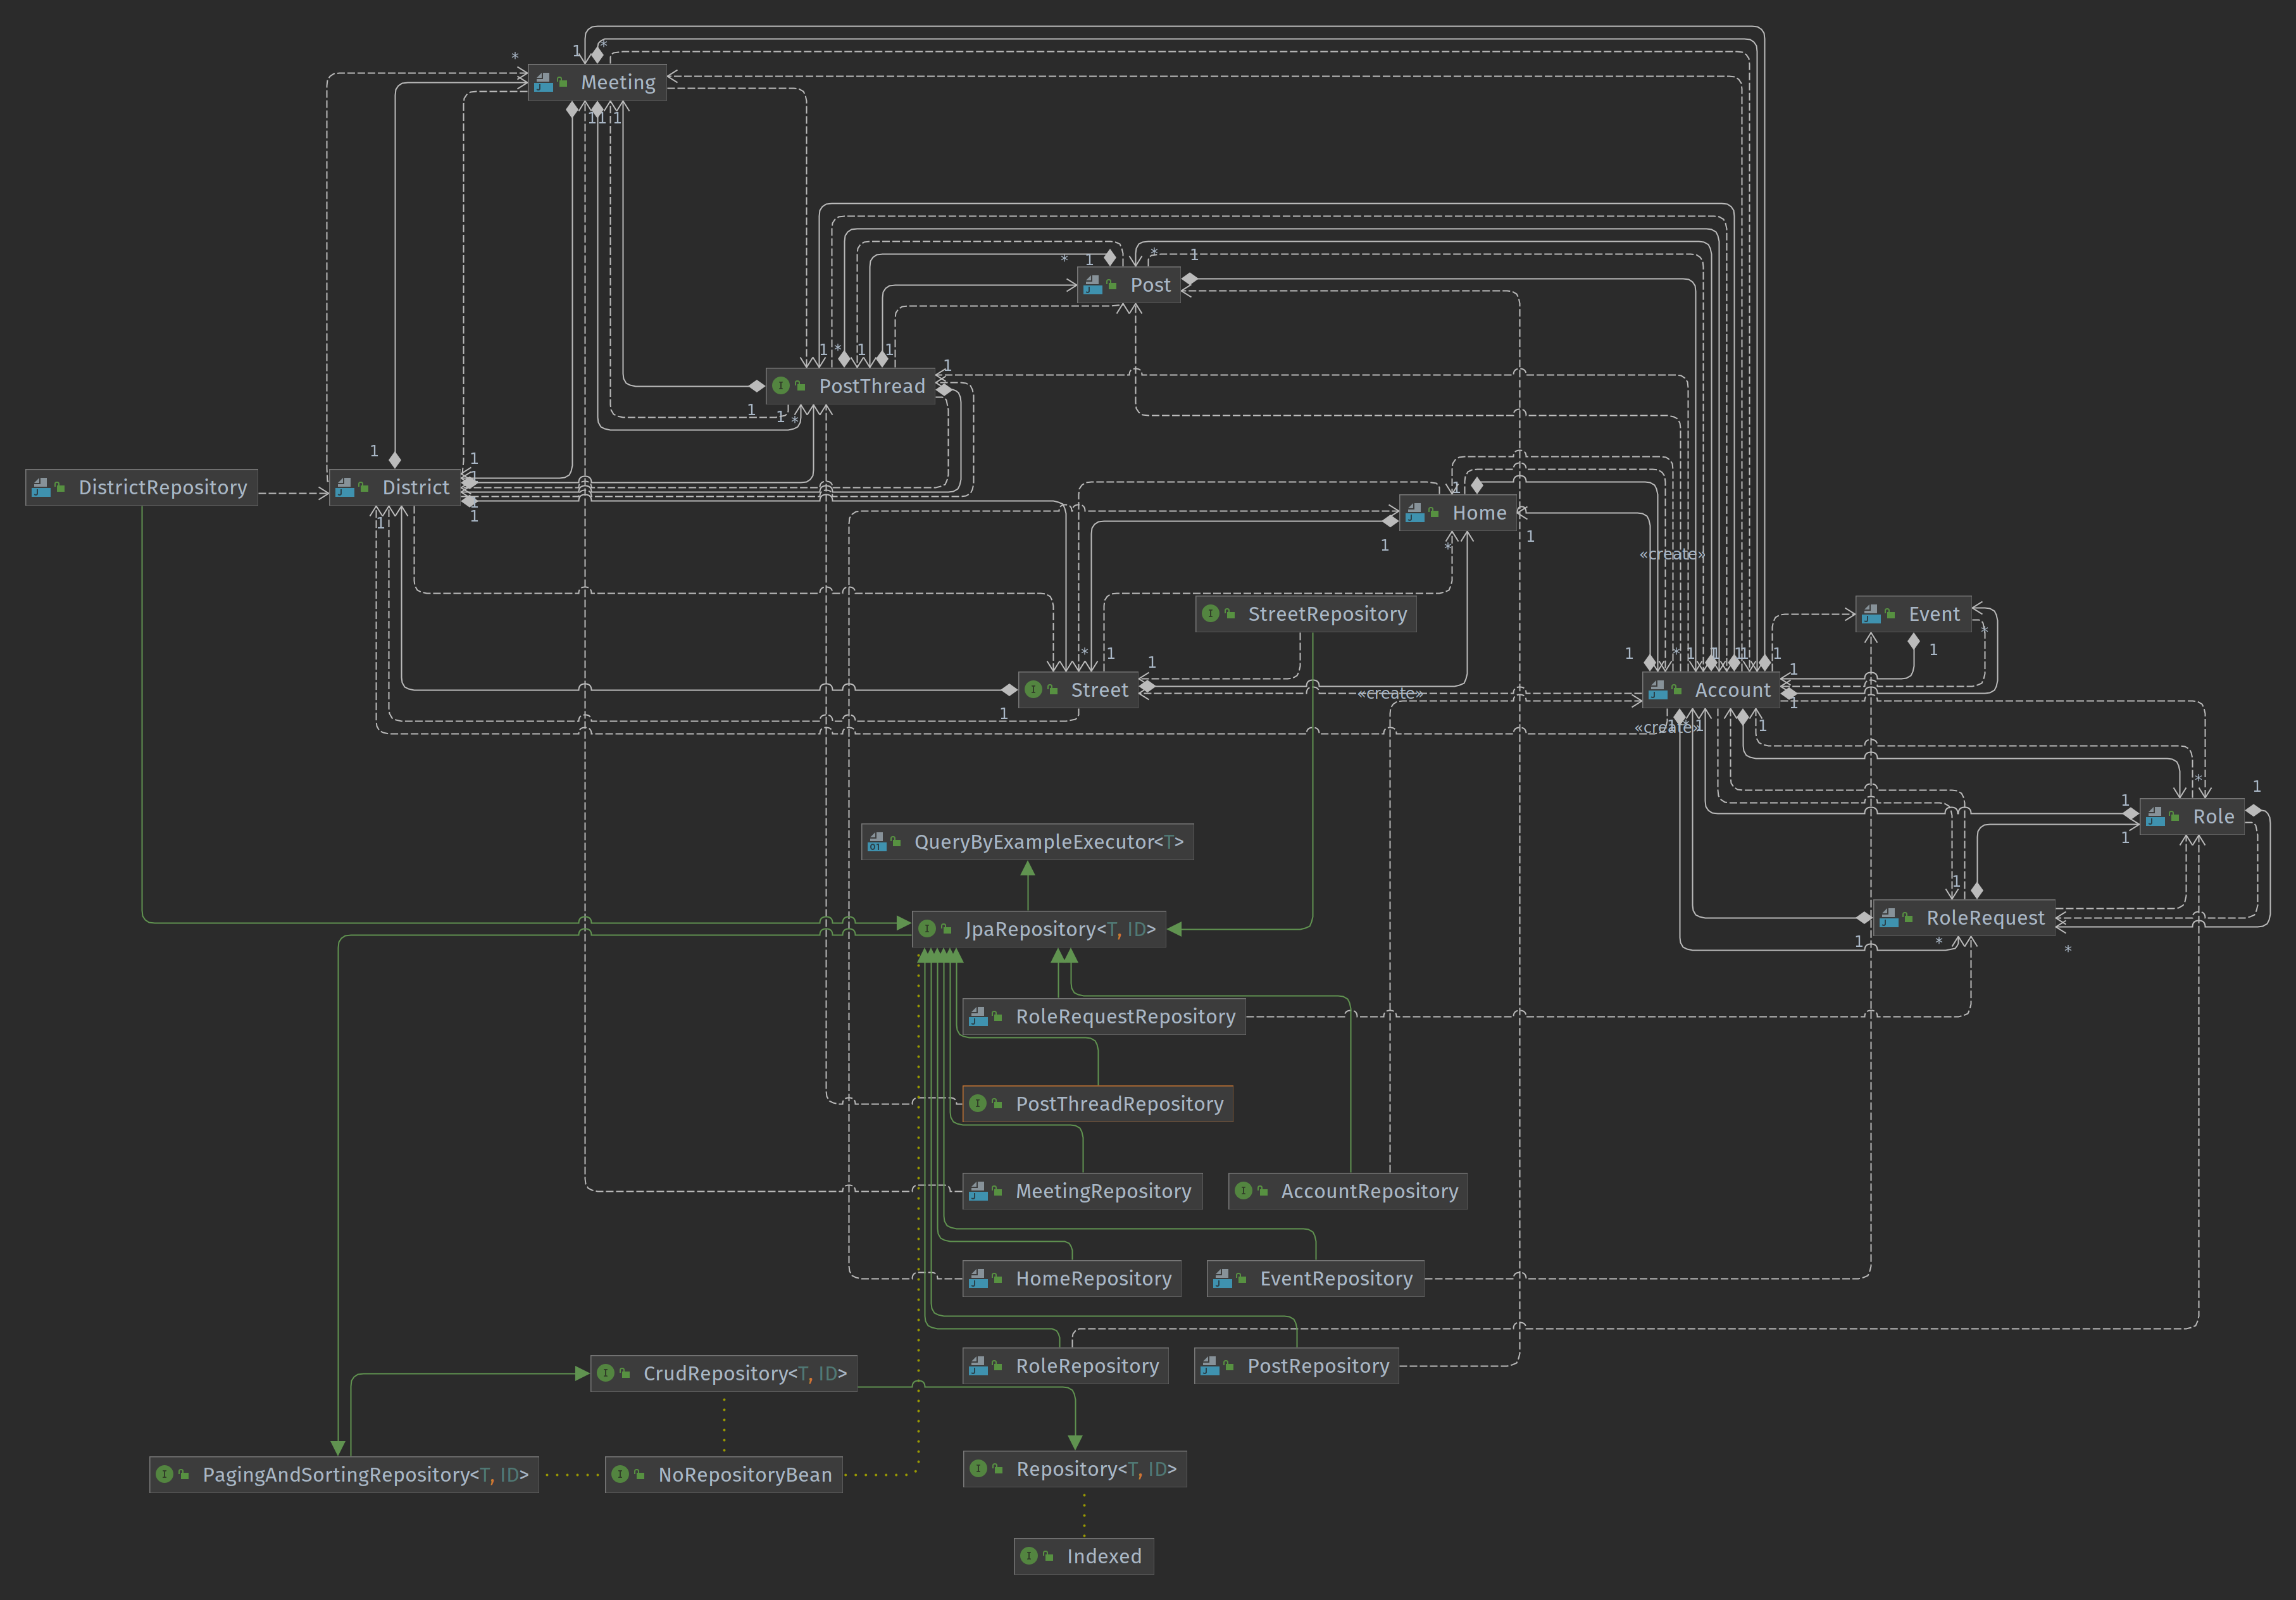
\includegraphics[width=\textwidth,keepaspectratio]{13.4 repozitoriji i entiteti.png}
					\caption{Dijagram razreda - odnos sloja Repository i entiteta}
				\end{figure}	
			
			
			\eject
			
		
		\section{Dijagram stanja}
		
		Na slici 4.10 prikazan je dijagram stanja korisničkog sučelja. Stranica na koju korisnik uvijek prvo dođe je "Prijava". S te stranice korisnik može birati opciju "Registracija" kako bi stvorio novi račun, ili se može prijaviti s postojećim računom. Ovisno o tome je li korisnik stanovnik ili administrator, dočeka ga prikladna početna stranica. 
		
		Ako je korisnik stanovnik, sa svoje početne stranice može birati opcije "Osobni podaci", "Događaji", "Vijeće četvrti" i "Forum". Pri pregledu svojih osobnih podataka, korisnik može slati zahtjeve za dodatne uloge ili mijenjati svoje osobne podatke. Pri pregledu sekcije "Događaji", korisnik može stvarati prijedloge događaja. Pri pregledu sekcije "Vijeće četvrti", korisnik klikom na pojedino izvješće može dobiti dodatne informacije o tom izvješću, a ako ima ulogu "Vijećnik", onda može i stvarati nova izvješća. Konačno, pregledom sekcije "Forum" korisnik može otvarati nove teme i pregledavati postojeće.
		
		Ako je korisnik administrator, sa svoje početne stranice može birati opcije "Osobni podaci", "Zahtjevi za uloge", "Korisnici" i "Kvartovi". Prilikom pregleda svojih osobnih podataka, administrator može neke od tih podataka može mijenjati. Prilikom pregleda zahtjeva za uloge administrator može odabrati pojedini zahtjev te ga prihvatiti ili odbiti. Prilikom pregleda svih korisnika sustava, administrator može odabrati pojedinog korisnika i dobiti više informacija o njemu. Konačno, pri pregledu kvartova, administrator može dodati novi kvart, a može i za postojeći kvart odabrati opciju unosa nove ulice.
		
		Iako zbog preglednosti to nije navedeno na dijagramu, stanovnici iz svih stanja mogu doći u stanja "Početna stranica", "Događaji", "Vijeće četvrti", "Forum" i "Osobni podaci", te administratori analogno mogu iz svih stanja doći u stanja "Početna stranica", "Korisnici", "Kvartovi", "Zahtjevi uloga" i "Osobni podaci". Također, svi korisnici iz svih stanja mogu birati opciju "Odjava" i preći u stanje "Prijava".
			
			
						\begin{figure}[H]
					\centering
					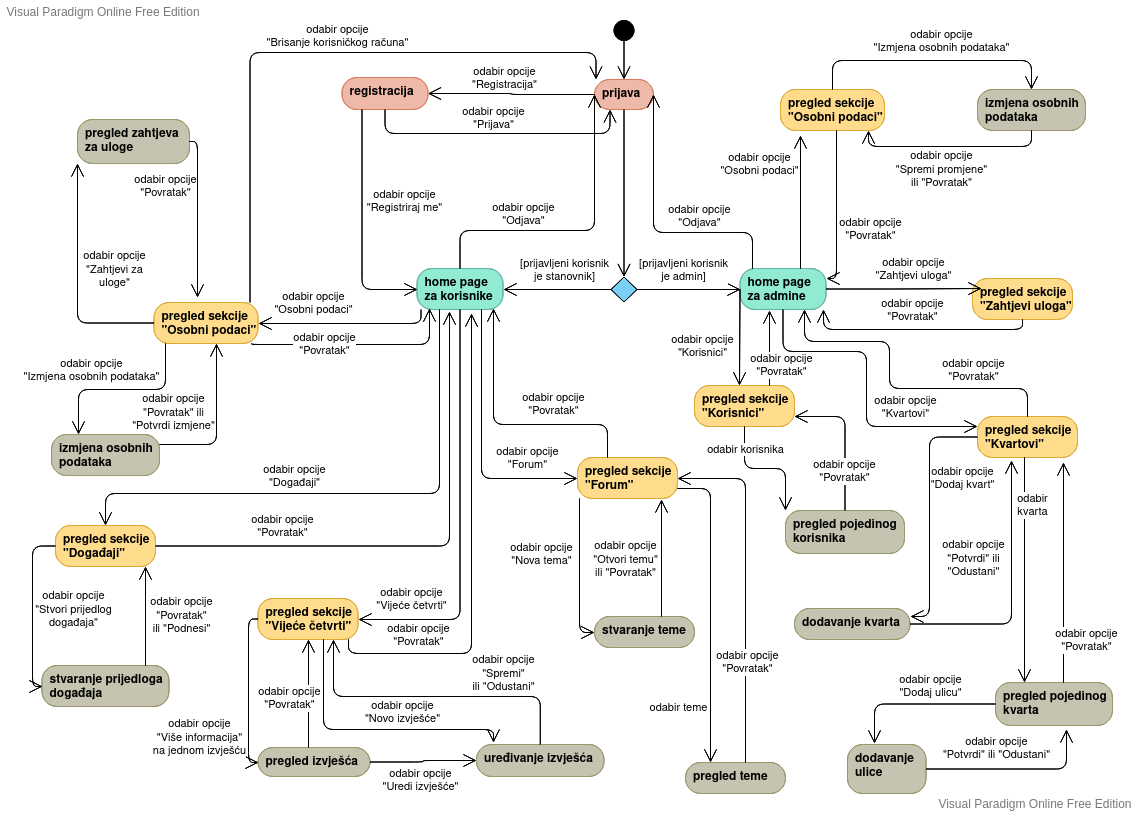
\includegraphics[width=\textwidth,keepaspectratio]{14 dijagram stanja.png}
					\caption{Dijagram stanja}
				\end{figure}	
			
			
			\eject 
		
		\section{Dijagram aktivnosti}
		
		Na slici 4.11 prikazan je dijagram aktivnosti prilikom stvaranja novih događaja. Korisnik koji želi predložiti događaj ispunjava formu u koju unosi naziv, mjesto, vrijeme, trajanje i kratki opis. Kada ju je ispunio, odabire opciju spremanja prijedloga. Web aplikacija tada provjerava jesu li svi traženi podaci u ispravnom formatu. Ako nisu, upozorava korisnika na pogreške i omogućuje mu da ih ispravi, a ako su podaci ispravni, onda sprema prijedlog u bazu podataka. Nakon što je prijedlog spremljen, moderator ga može pregledati. Ako moderator procijeni da prijedlog ne zadovoljava jezični standard, može ga uređivati. Kada je ispravio sve eventualne pogreške, moderator odabire opciju spremanja promjena. Tada web aplikacija provjerava jesu li svi podaci u ispravnom formatu, te ako jesu, sprema promjene, a ako nisu, upozorava moderatora na pogreške i omogućuje mu da ih ispravi. Nakon što je završio s eventualnim uređivanjem prijedloga, moderator može odabrati opciju prihvaćanja ili odbijanja prijedloga, i u oba slučaja se ažurira status prijedloga događaja u bazi podataka.
			
			\begin{figure}[H]
					\centering
					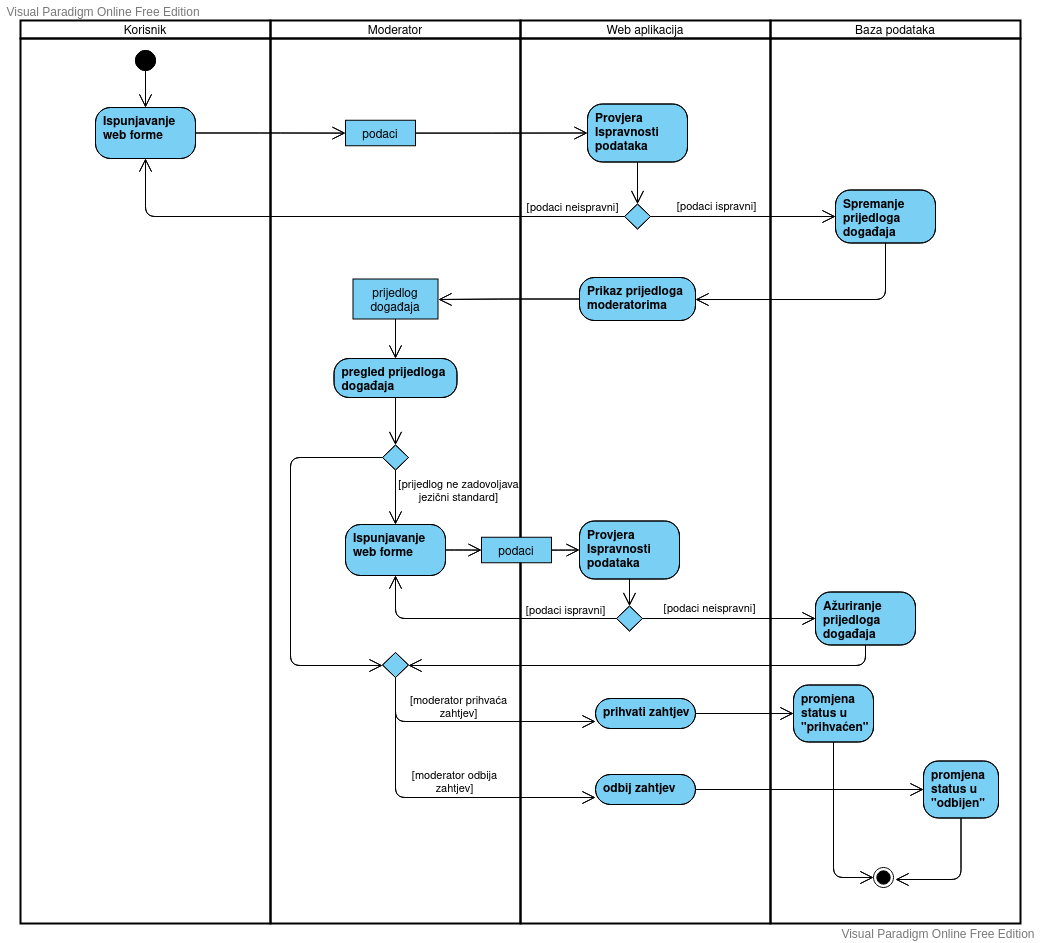
\includegraphics[width=\textwidth,keepaspectratio]{15 dijagram aktivnosti.png}
					\caption{Dijagram aktivnosti}
				\end{figure}	
			
			\eject
		\section{Dijagram komponenti}
		
		 Na slici 4.12 prikazan je dijagram komponenti. Korisnik iz web preglednika pristupa pristupa aplikaciji korištenjem REST API-ja. Sama aplikacija se sastoji od dvije komponente. Prva komponenta odgovara frontendu i izgrađena je korištenjem React biblioteke. Druga komponenta odgovara backendu i izgrađena je korištenjem radnog okvira Spring. Frontend i backend komuniciraju korištenjem REST API-ja. Baza podataka je relacijska i backend joj pristupa slanjem SQL upita.
		
			\begin{figure}[H]
					\centering
					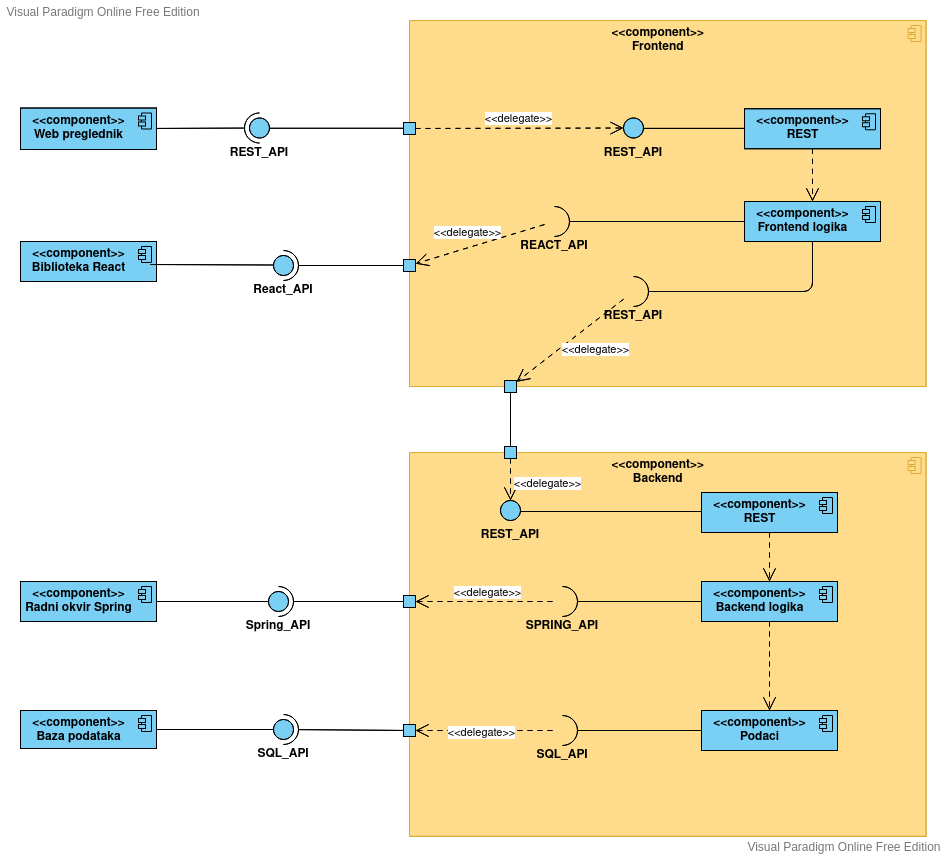
\includegraphics[width=\textwidth,keepaspectratio]{16 dijagram komponenti.png}
					\caption{Dijagram komponenti}
				\end{figure}	
				\newpage			

	\chapter{Implementacija i korisničko sučelje}
		
		
		\section{Korištene tehnologije i alati}
		
			Komunikacija u timu je ostvarena korištenjem aplikacije Discord\footnote{\url{https://discord.com/}}. Komunikacija s asistenticom grupe je ostvarena korištenjem aplikacije Microsoft Teams\footnote{\url{https://www.microsoft.com/hr-hr/microsoft-teams/group-chat-software/}} Za izradu UML dijagrama korišten je alat Visual Paradigm Online\footnote{\url{https://online.visual-paradigm.com/}}. Za upravljanje izvornim kodom korišten je alat Git\footnote{\url{https://git-scm.com/}}. Udaljeni repozitorij projekta nalazi se na platformi Gitlab\footnote{\url{https://gitlab.com/}}. Za upravljanje zadacima na projektu korištena je aplikacija Trello\footnote{\url{https://trello.com/}}.
			
			Kao razvojno okruženje na backendu je koršten IntelliJ\footnote{\url{https://www.jetbrains.com/idea/}}, a na frontendu je korišten Visual Studio Code\footnote{\url{https://code.visualstudio.com/}}. Tehnologije korištene za razvoj backenda su radni okvir Spring Boot\footnote{\url{https://spring.io/projects/spring-boot}} i programski jezik Java\footnote{\url{https://www.java.com/en/}}. Tehologije korištene za razvoj frontenda su biblioteka React\footnote{\url{https://reactjs.org/}} i programski jezik JavaScript\footnote{\url{https://www.javascript.com/}}. Za automatizirano testiranje korišten je alat Selenium WebDriver\footnote{\url{https://www.selenium.dev/documentation/webdriver/}} te programski jezici Java i Python\footnote{\url{https://www.python.org/}}. Za puštanje aplikacije u pogon korištena je platforma Heroku\footnote{\url{https://www.heroku.com/}}.
			
			
			\eject 
		
	
		\section{Ispitivanje programskog rješenja}
					
			\subsection{Ispitivanje komponenti}

			Ispitivanje komponenti ostvareno je korištenjem Spring Boot i JUnit alata za ispitivanje.
			U nastavku su opisani provedeni testovi, te su priloženi kodovi.

			Testovi 1-4 testiraju Account kontroler.
			Inicijalizacijska metoda za testove 1-4 izgleda ovako:

			\begin{lstlisting}[language=Java, breaklines=true]
    @BeforeEach
    public void init() {
        Street street = new Street(1L, "Testna ulica", 1, 5);
        street.setDistrict(new District(1L, "Testni kvart"));
        home = new Home(1L, 1L, street);

        account = new Account(1L, "John", "Doe", "johndoe@gmail.com", "pass123",
                home, null, false);
        account.setRoles(new ArrayList<>());
    }
			\end{lstlisting}

			Testovi 5 i 6 testiraju Post kontroler.
			Inicijalizacijska metoda za testove 5 i 6 izgleda ovako:

			\begin{lstlisting}[language=Java, breaklines=true]
    @BeforeEach
    public void init() {
        District district = new District(1L, "Testni kvart");
        Street street = new Street(1L, "Testna ulica", 1, 5);
        street.setDistrict(district);
        home = new Home(1L, 1L, street);

        account = new Account(1L, "John", "Doe", "johndoe@gmail.com", "pass123",
                home, null, false);

        postThread = new PostThread(1L, "Example", new ArrayList<>(), null, district);

        post = new Post(1L, "First post",
                null,
                null, postThread, account);

        post.setThreadId(postThread.getId());
    }
			\end{lstlisting}

			U prvom ispitnom slučaju ispitan je pokušaj dobavljanja liste svih korisničkih računa.
			Očekivani rezultat je uspješno dobavljanje liste u JSON obliku te HTTP status 200 (OK).

			\begin{lstlisting}[language=Java, breaklines=true]
    @Test
    public void givenAccountsList_whenGetAccountsList_ThenReturnJsonArray() throws Exception {
        List<Account> accounts = Collections.singletonList(account);

        given(accountService.listAll()).willReturn(accounts);

        mvc.perform(get("/accounts")
                .contentType(MediaType.APPLICATION_JSON).accept(MediaType.APPLICATION_JSON))
                .andExpect(status().isOk())
                .andExpect(jsonPath("$", hasSize(1)))
                .andExpect(jsonPath("$[0].firstName").value("John"));
    }
			\end{lstlisting}

			U drugom ispitnom slučaju testiran je rubni slučaj u kojem ne postoji niti jedan korisnički račun, a lista
			korisničkih računa se pokušava dohvatiti. Očekivani rezultat je uspješno dobavljanje prazne liste u JSON obliku te HTTP status 200 (OK).

			\begin{lstlisting}[language=Java, breaklines=true]
	@Test
    public void givenEmptyAccountsList_whenGetAccountsList_thenReturnEmptyJsonArray() throws Exception {
        List<Account> accounts = Collections.emptyList();

        given(accountService.listAll()).willReturn(accounts);

        mvc.perform(get("/accounts")
                .contentType(MediaType.APPLICATION_JSON).accept(MediaType.APPLICATION_JSON))
                .andExpect(status().isOk())
                .andExpect(jsonPath("$", empty()));
    }
			\end{lstlisting}

			U trećem ispitnom slučaju ispitan je pokušaj izrade novog korisničkog računa, dok je pritom priložena email adresa koju neki postojeći korisnik već koristi. Očekivani rezultat je neuspješna izrada korisničkog računa te HTTP status 400 (Bad Request).

			\begin{lstlisting}[language=Java, breaklines=true]
    @Test
    public void givenEmailList_whenCreateAccountWithExistingEmail_thenCauseError400() throws Exception {
        given(accountService.getEmailsFromAccounts()).willReturn(Collections.singletonList("johndoe@gmail.com"));

        mvc.perform(post("/accounts")
                .content(new ObjectMapper()
                        .writeValueAsString(new Account("Johnny", "Doe",
                                "johndoe@gmail.com", "pass123", home, null,
                                false)
                        )
                ).contentType(MediaType.APPLICATION_JSON).accept(MediaType.APPLICATION_JSON)
        ).andExpect(status().isBadRequest());
    }
			\end{lstlisting}

			U četvrtom ispitnom slučaju ispitan je pokušaj dodjele uloge "Stanovnik" postojećem korisniku preko "/accounts/grantRole/" endpointa.
			Očekivani rezultat je uspješna dodjela uloge "Stanovnik" korisniku te HTTP status 200 (OK).

			\begin{lstlisting}[language=Java, breaklines=true]
    @Test
    public void whenGrantRole_thenReturnRole() throws Exception {
        given(accountService.fetch(any(Long.class))).willReturn(account);
        given(accountService.existsById(eq(1L))).willReturn(true);
        given(roleService.findByName(any(String.class))).willReturn(java.util.Optional.of(new Role("Stanovnik")));

        mvc.perform(put("/accounts/grantRole/{id}",1)
                .content("Stanovnik").contentType(MediaType.APPLICATION_JSON).accept(MediaType.APPLICATION_JSON)
        ).andExpect(status().isOk())
                .andExpect(jsonPath("$.name").value("Stanovnik"));
    }
			\end{lstlisting}

			U petom ispitnom slučaju ispitan je pokušaj izrade nove objave uz priložen tekst objave i priložen id postojeće dretve. Očekivani rezultat je uspješna izrada nove objave koja sadrži priložen tekst, te HTTP status 201 (Created).

			\begin{lstlisting}[language=Java, breaklines=true]
    @Test
    public void givenPost_whenCreatePost_thenReturnPostAsJson() throws Exception {
        Post post2 = new Post(2L, "Second post",
                null,
                null, postThread, account);

        post2.setThreadId(postThread.getId());
        given(accountService.fetch(any(Long.class))).willReturn(account);
        given(postService.createPost(any(Post.class), eq(postThread.getId()))).willReturn(post2);
        given(postService.existsById(eq(post2.getId()))).willReturn(false);
        given(postThreadService.existsById(eq(postThread.getId()))).willReturn(true);

        mvc.perform(post("/posts/{id}",1)
                .content(new ObjectMapper().writeValueAsString(post2))
                .contentType(MediaType.APPLICATION_JSON).accept(MediaType.APPLICATION_JSON))
                .andExpect(status().isCreated())
                .andExpect(jsonPath("$.id").value(2))
                .andExpect(jsonPath("$.content").value("Second post"));
    }
			\end{lstlisting}

			U šestom ispitnom slučaju ispitan je pokušaj dohvaćanja objave preko nepostojećeg id-a.
			Očekivani rezultat je neuspješno dohvaćanje objave te HTTP status 400 (Bad Request).

			\begin{lstlisting}[language=Java, breaklines=true]
    @Test
    public void givenNonexistentPostId_whenGetPost_thenCauseError400() throws Exception {
        given(postService.existsById(any(Long.class))).willReturn(false);

        mvc.perform(get("/posts/{id}",5)
                .contentType(MediaType.APPLICATION_JSON)
                .accept(MediaType.APPLICATION_JSON)
        ).andExpect(status().isBadRequest());
    }
			\end{lstlisting}

			Na slici 5.1 je prikazana je snimka zaslona terminala u IntelliJ IDE-u, kao rezultat izvođenja prethodno navedenih šest ispitnih slučajeva.

			\begin{figure}[H]
					\centering
					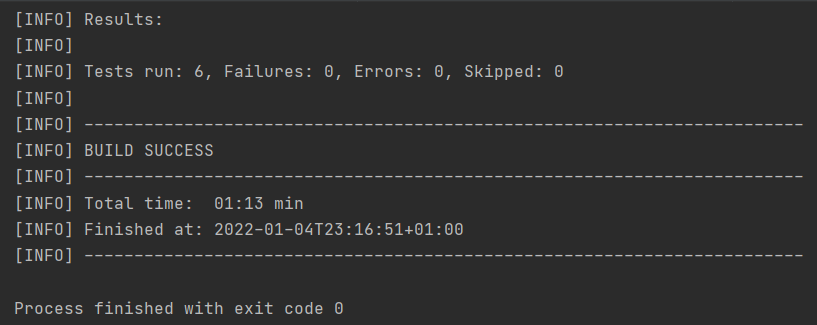
\includegraphics[width=\textwidth,keepaspectratio]{19 ispitivanje komponenti.png}
					\caption{Rezultati ispitivanja pomoću Spring-a i JUnit-a}
				\end{figure}
			\eject

			\subsection{Ispitivanje sustava}

			Ispitivanje sustava ostvareno je korištenjem Selenium WebDrivera i programskog jezika Python. U nastavku su opisani provedeni testovi, te su priloženi kodovi.

			U prvom ispitnom slučaju ispitan je pokušaj prijave s emailom koji nije povezan niti jedan račun, tj. emailom koji ne postoji u sustavu. Očekivani izlaz je neuspjeh pri pokušaju prijave.

			\begin{lstlisting}[language=Python, breaklines=true]
def test1() -> bool:
    driver = webdriver.Firefox()
    driver.get("http://localhost:3000/login")
    driver.find_element_by_name("username").send_keys("stanovnik@stanovnik.com")
    driver.find_element_by_name("password").send_keys("stanovnik")
    driver.find_element_by_css_selector("button[type='submit']").click()
    try:
        driver.find_element_by_class_name("logout")
    except NoSuchElementException:
        driver.close()
        return True
    driver.close()
    return False
			\end{lstlisting}

			U drugom ispitnom slučaju ispitan je pokušaj registracije s neispravnim podacima, konkretno s emailom koji je zadan u krivom formatu. Očekivani izlaz je neuspjeh pri pokušaju registracije.

			\begin{lstlisting}[language=Python, breaklines=true]
def test2() -> bool:
    driver = webdriver.Firefox()
    driver.get("http://localhost:3000/login")
    driver.find_element_by_css_selector("button[type='button']").click()
    driver.find_element_by_name("firstname").send_keys("Stanovnik")
    driver.find_element_by_name("lastname").send_keys("Stanovnikic")
    driver.find_element_by_name("username").send_keys("stanovnik")
    driver.find_element_by_name("password").send_keys("stanovnik")
    dropdown = driver.find_element_by_class_name("css-tlfecz-indicatorContainer")
    dropdown.click()
    actions = ActionChains(driver)
    actions.move_to_element(dropdown).send_keys("Ulica 1 Kvarta 1").key_down(Keys.ENTER).key_up(Keys.ENTER).perform()
    driver.find_element_by_name("streetnumber").send_keys("7")
    driver.find_element_by_css_selector("button[type='submit']").click()
    try:
        driver.find_element_by_class_name("logout")
    except NoSuchElementException:
        driver.close()
        return True
    driver.close()
    return False
			\end{lstlisting}

			U trećem ispitnom slučaju ispitan je pokušaj registracije gdje su svi uneseni podaci valjani. Očekivani izlaz je uspjeh pri pokušaju registracije i preusmjeravanje na početnu stranicu korisnikovog kvarta.

			\begin{lstlisting}[language=Python, breaklines=true]
def test3() -> bool:
    driver = webdriver.Firefox()
    driver.get("http://localhost:3000/login")
    driver.find_element_by_css_selector("button[type='button']").click()
    driver.find_element_by_name("firstname").send_keys("Stanovnik")
    driver.find_element_by_name("lastname").send_keys("Stanovnikic")
    driver.find_element_by_name("username").send_keys("stanovnik@stanovnik.com")
    driver.find_element_by_name("password").send_keys("stanovnik")
    dropdown = driver.find_element_by_class_name("css-tlfecz-indicatorContainer")
    dropdown.click()
    actions = ActionChains(driver)
    actions.move_to_element(dropdown).send_keys("Ulica 1 Kvarta 1").key_down(Keys.ENTER).key_up(Keys.ENTER).perform()
    driver.find_element_by_name("streetnumber").send_keys("7")
    driver.find_element_by_css_selector("button[type='submit']").click()
    try:
        driver.find_element_by_class_name("logout")
    except NoSuchElementException:
        driver.close()
        return False
    driver.close()
    return True
			\end{lstlisting}

			U četvrtom ispitnom slučaju ispitan je pokušaj prijave s emailom za koji postoji korisnički račun, ali s neispravnom lozinkom. Očekivani izlaz je neuspjeh pri pokušaju prijave.

			\begin{lstlisting}[language=Python, breaklines=true]
def test4() -> bool:
    driver = webdriver.Firefox()
    driver.get("http://localhost:3000/login")
    driver.find_element_by_name("username").send_keys("stanovnik@stanovnik.com")
    driver.find_element_by_name("password").send_keys("stanovni")
    driver.find_element_by_css_selector("button[type='submit']").click()
    try:
        driver.find_element_by_class_name("logout")
    except NoSuchElementException:
        driver.close()
        return True
    driver.close()
    return False
			\end{lstlisting}

			U petom ispitnom slučaju ispitan je pokušaj prijave gdje su svi uneseni podaci ispravni. Očekivani izlaz je uspjeh pri pokušaju prijave i preusmjeravanje na početnu stranicu korisnikovog kvarta.

			\begin{lstlisting}[language=Python, breaklines=true]
def test5() -> bool:
    driver = webdriver.Firefox()
    driver.get("http://localhost:3000/login")
    driver.find_element_by_name("username").send_keys("stanovnik@stanovnik.com")
    driver.find_element_by_name("password").send_keys("stanovnik")
    driver.find_element_by_css_selector("button[type='submit']").click()
    try:
        driver.find_element_by_class_name("logout")
    except NoSuchElementException:
        driver.close()
        return False
    driver.close()
    return True
			\end{lstlisting}

			Na slici 5.2 prikazana je snimka zaslona terminala kao rezultat izvođenja prethodno navedenih pet ispitnih slučajeva.

			\begin{figure}[H]
					\centering
					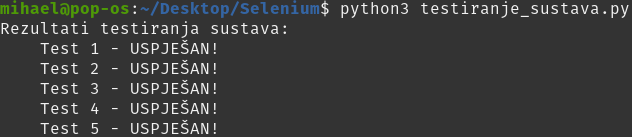
\includegraphics[width=\textwidth,keepaspectratio]{18 ispitivanje sustava.png}
					\caption{Rezultati ispitivanja Selenium WebDriverom}
				\end{figure}
			\eject


		\section{Dijagram razmještaja}

		Na slici 5.3 prikazan je dijagram razmještaja. Sustav je baziran na arhitekturi "klijent-poslužitelj". Korisnici pristupaju aplikaciji korištenjem web preglednika. Na platformi Heroku se nalaze poslužitelji za frontend, backend i bazu podataka. Komunikacija između korisnika i poslužitelja za frontend, te poslužitelja za frontend i poslužitelja za backend, ostvaruje se korištenjem protokola HTTP.

			\begin{figure}[H]
					\centering
					\includegraphics[width=\textwidth,keepaspectratio]{17 dijagram razmještaja.png}
					\caption{Dijagram razmještaja}
				\end{figure}

			\eject

		\section{Upute za puštanje u pogon}
		
		
		Potrebno je napraviti korisnički račun na Heroku i zatim odabirom opcije "New app" stvoriti dvije aplikacije, jednu za frontend i jednu za backend.
		
		S obzirom da je puštanje u pogon značajno jednostavnije s Githuba nego s Gitlaba, potrebno je neki, npr. osobni Github račun, povezati s Heroku računom i potom klonirati projekt dva puta. U prvom kloniranom projektu je potrebno u root direktorij premjestiti sadržaj poddirektorija IzvorniKod/backend-spring-boot, a ostatak sadržaja projekta obrisati. U drugom je projektu potrebno učiniti istu stvar za sadržaj poddirektorija IzvorniKod/frontend-react. Zatim je u svakom projektu na main grani potrebno odabrati opciju "Deploy to Heroku". 
		
		Na Heroku Vas dočeka stranica poput one na slici 5.4. Kada ste u pogon pustili frontend i backend, potrebno je u datoteku .env.production na frontend projektu napisati točan URL na kojem se nalazi backend. Primjer je pokazan na slici 5.5.

		Konačni je korak napuniti bazu s nekom .sql skriptom. Pri puštanju u pogon backenda, automatski se stvori i baza podataka. Na slici 5.4 vidljiva je poveznica "Resources". Potrebno je odabrati ju, zatim je potrebno pod "add-ons" odabrati "heroku postgres" i dočekaju Vas podaci slični onima na slici 5.6. Zatim je potrebno otvoriti pgAdmin, i odabrati opciju "Create Server", kao što je prikazano na slici 5.7. Dalje je potrebno slijediti upute i unijeti podatke poput onih na slici 5.6, i konačno, kada je baza podataka povezana lokalno s pgAdminom, potrebno je odabirom na "Query tool" unijeti željenu .sql skriptu.
		
				\begin{figure}[H]
					\centering
					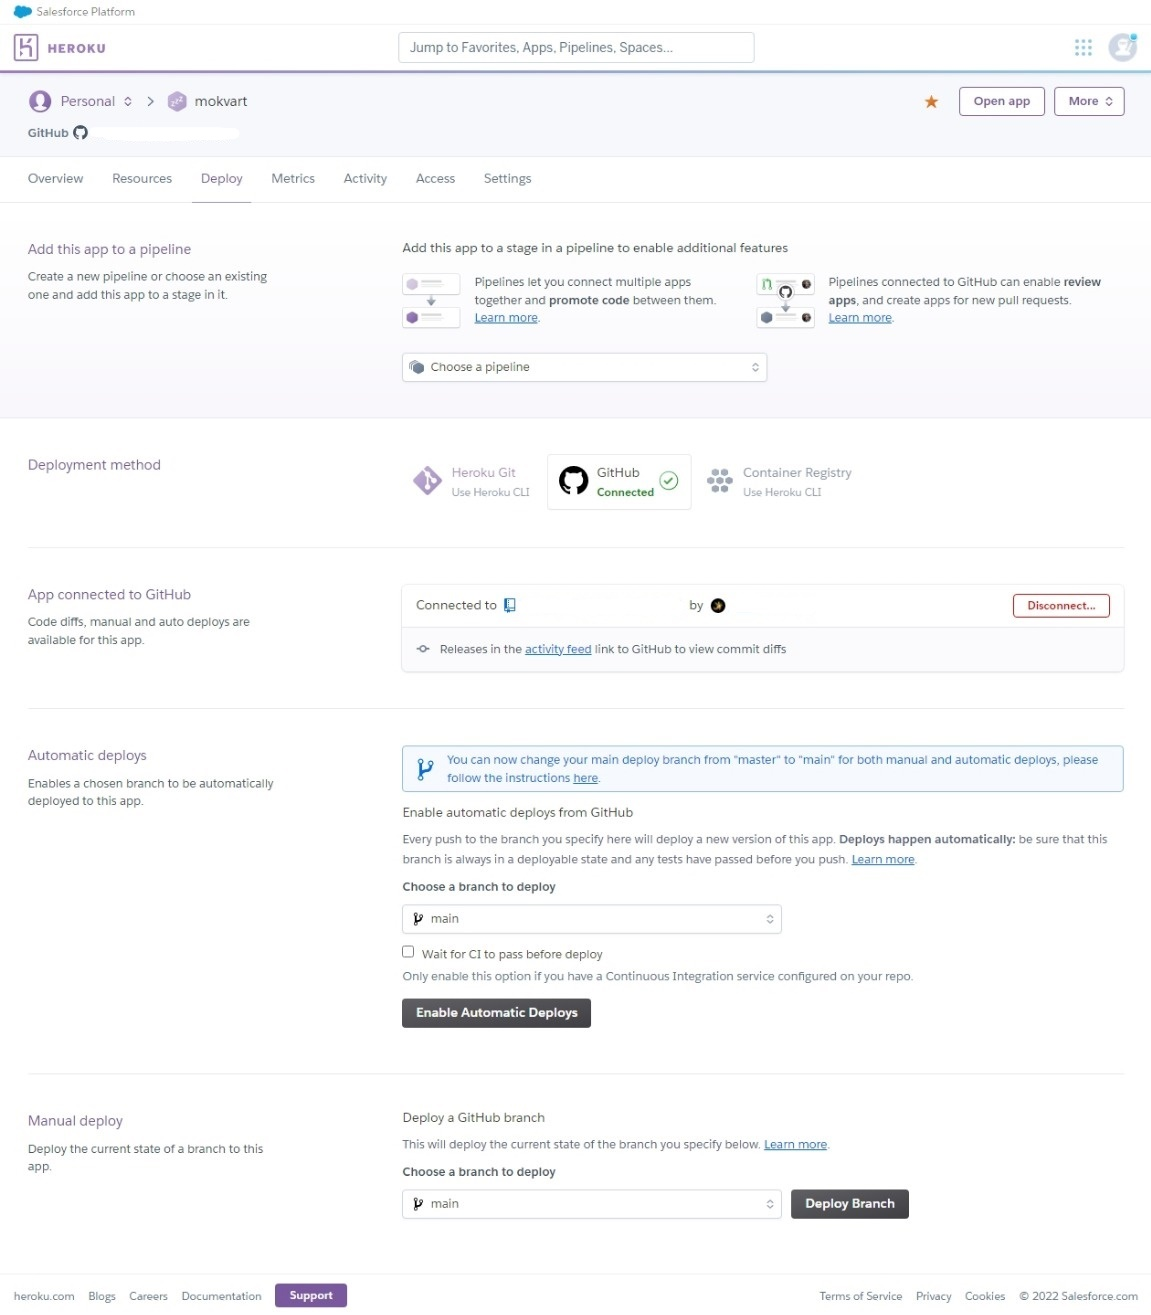
\includegraphics[width=\textwidth,keepaspectratio]{20 heroku screenshot.png}
					\caption{Prikaz aplikacije na poslužitelju Heroku}
				\end{figure}
				
				\begin{figure}[H]
					\centering
					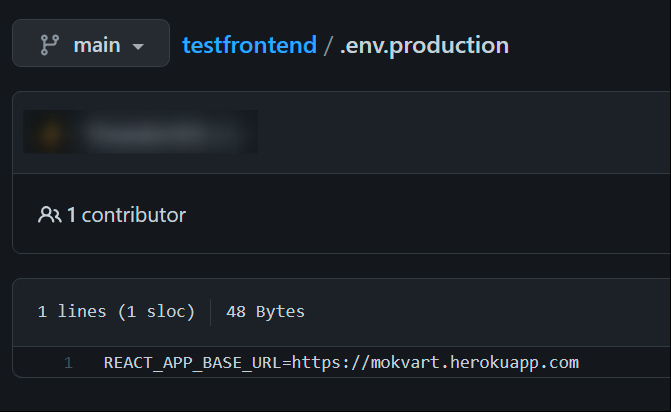
\includegraphics[width=\textwidth,keepaspectratio]{21 URL config.png}
					\caption{Povezivanje frontenda i backenda}
				\end{figure}
				
				\begin{figure}[H]
					\centering
					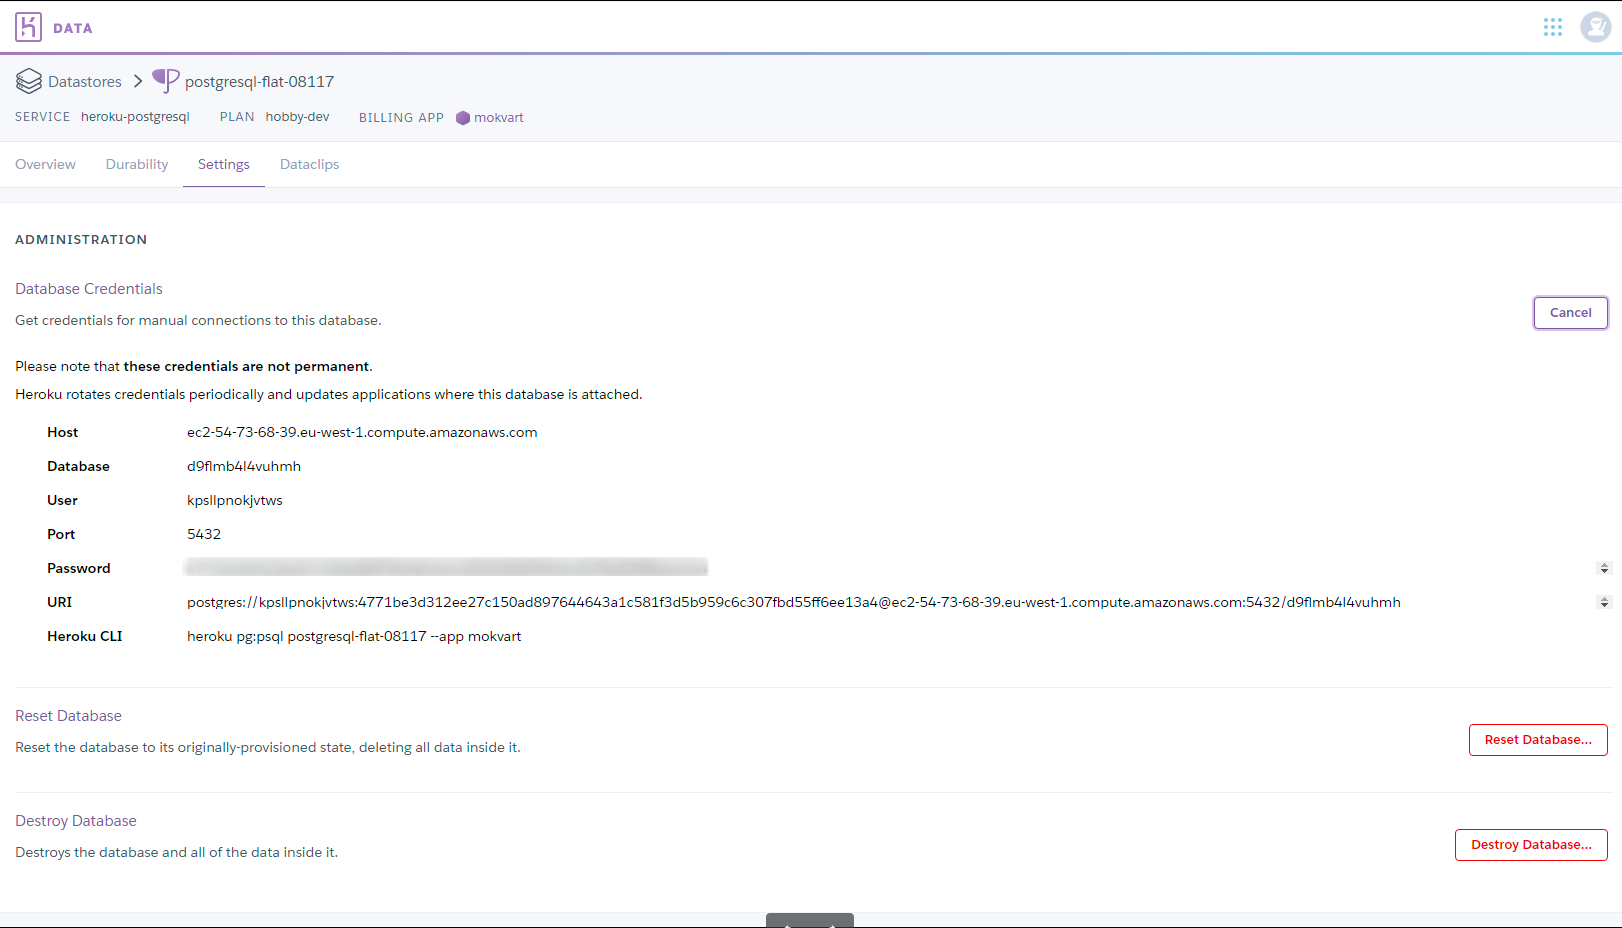
\includegraphics[width=\textwidth,keepaspectratio]{22 baza podaci.png}
					\caption{Podaci za pristup bazi}
				\end{figure}
				
				\begin{figure}[H]
					\centering
					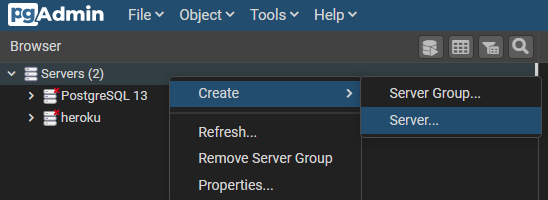
\includegraphics[width=\textwidth,keepaspectratio]{23 baza povezivanje.png}
					\caption{Pristup bazi lokalno u pgAdminu}
				\end{figure}

			\eject
	\chapter{Zaključak i budući rad}
		
		Zadatak naše grupe bio je razvoj web aplikacije pod nazivom "Moj kvart". Ideja aplikacije je da bude svojevrsna društvena mreža preko koje stanovnici istih kvartova mogu komunicirati, komentirati neke teme na forumu, predlagati grupne događaje i slično. Nakon 12 tjedana timskog rada, ostvarili smo zadani cilj i projekt je završen. Projekt je imao tri faze.
		
		Prva faza je uključivala okupljanje tima, razgovor o generalnim idejama za aplikaciju, izražavanje pojedinačnih interesa i želja za radom u prvom ciklusu predaje, te konačno podjela zadataka za prvi ciklus. Formirala su se dva podtima. U prvom podtimu su članovi radili na dokumentiranju zahtjeva, obrazaca uporabe, UML dijagrama te bazi podataka. U drugom podtimu su članovi istraživali, proučavali i eskperimentirali s tehnologijama u kojima će kasnije biti implementirana aplikacija. Prva je faza projekta trajala do kolokviranja prvog ciklusa projekta.
		
		U drugoj je fazi naglasak bio na implementaciji aplikacije, i ovdje nije bilo podtimova nego su svi članovi zajedno radili na programskom ostvarenju aplikacije. U ovoj je fazi implementirana većina aplikacije, a trajala je do demonstracije alfa inačice aplikacije.
		
		Treća i konačna faza je uključivala izradu raznih UML dijagrama, ispitivanje sustava, pronalazak i ispravak grešaka, rad na izgledu aplikacije i implementacija preostalih funkcionalnosti. U ovoj fazi je postojalo dosta manjih zadataka koje je trebalo napraviti, pa su članovi tima uglavnom samostalno preuzimali te zadatke i obavljali ih. Ova je faza trajala do završetka projekta, prije konačne predaje i kolokviranja drugog ciklusa.
		
		Projekt je moguće proširiti na mnogo načina. Jedna od ideja je u Forum dodati više funkcionalnosti, tako da korisnici mogu pregledati druge korisnike i sve njihove objave, te da dobivaju obavijesti kada im netko odgovori na objavu. Drugo proširenje koje bi doprinijelo kvaliteti aplikacije je mogućnost da korisnici šalju izravno poruke drugim korisnicima.
		
		Sudjelovanje u ovom projektu je bilo vrijedno iskustvo za sve članove tima. Svima nama je ovo bio prvi ozbiljniji grupni projekt, i snašli smo se jako dobro. Konflikata u timu gotovo da nije bilo, a suradnja i komunikacija su bili na iznimno zadovoljavajućoj razini. Većini nas je ovaj projekt bio prvi ozbiljniji dodir s tehnologijama poput Gita i Latex. Naučili smo koristiti neke moderne radne okvire pri izradi web aplikacija. Iznimno smo zadovoljni postignutim rezultatima i timskim radom koji je do tih rezultata doveo.
		
		\eject 
	\chapter*{Popis literature}
		\addcontentsline{toc}{chapter}{Popis literature}
	 	
 		\textbf{\textit{Kontinuirano osvježavanje}}
	
		\textit{Popisati sve reference i literaturu koja je pomogla pri ostvarivanju projekta.}
		
		
		\begin{enumerate}
			
			
			\item  Programsko inženjerstvo, FER ZEMRIS, \url{http://www.fer.hr/predmet/proinz}
			
			\item  I. Sommerville, "Software engineering", 8th ed, Addison Wesley, 2007.
			
			\item  T.C.Lethbridge, R.Langaniere, "Object-Oriented Software Engineering", 2nd ed. McGraw-Hill, 2005.
			
			\item  I. Marsic, Software engineering book``, Department of Electrical and Computer Engineering, Rutgers University, \url{http://www.ece.rutgers.edu/~marsic/books/SE}
			
			\item  The Unified Modeling Language, \url{https://www.uml-diagrams.org/}
			
			\item  Astah Community, \url{http://astah.net/editions/uml-new}
		\end{enumerate}
		
		 
	
	
	\begingroup
	\renewcommand*\listfigurename{Indeks slika i dijagrama}
	%\renewcommand*\listtablename{Indeks tablica}
	%\let\clearpage\relax
	\listoffigures
	%\vspace{10mm}
	%\listoftables
	\endgroup
	\addcontentsline{toc}{chapter}{Indeks slika i dijagrama}


	
	\eject 
		
	\chapter*{Dodatak: Prikaz aktivnosti grupe}
		\addcontentsline{toc}{chapter}{Dodatak: Prikaz aktivnosti grupe}
		
		\section*{Dnevnik sastajanja}
		
		
		\begin{packed_enum}
			\item  sastanak
			
			\item[] \begin{packed_item}
				\item Datum: 3.10.2021.
				\item Prisustvovali: Andrija Banić, Danijel Barišić, Danko Čurlin, Bartol Hrg, Mihael Miličević, Dario Pavlović, Tomislav Žiger
				\item Teme sastanka:
				\begin{packed_item}
					\item  formiranje tima
					\item  dogovor o imenu tima
					\item  dogovor o korištenim tehnologijama
				\end{packed_item}
			\end{packed_item}
			
			\item  sastanak
			\item[] \begin{packed_item}
				\item Datum: 13.10.2021.
				\item Prisustvovali: Andrija Banić, Danijel Barišić, Danko Čurlin, Dario Pavlović
				\item Teme sastanka:
				\begin{packed_item}
					\item  s asistenticom grupe raspravljali o osnovnim pitanjima na projektu
				\end{packed_item}
			\end{packed_item}
			
			\item  sastanak
			\item[] \begin{packed_item}
				\item Datum: 14.10.2021.
				\item Prisustvovali: Andrija Banić, Danijel Barišić, Danko Čurlin, Bartol Hrg, Mihael Miličević, Dario Pavlović, Tomislav Žiger
				\item Teme sastanka:
				\begin{packed_item}
					\item  okvirna podjela zadataka na projektu u prvom ciklusu predaje
				\end{packed_item}
			\end{packed_item}
			
			\item  sastanak
			\item[] \begin{packed_item}
				\item Datum: 15.10.2021.
				\item Prisustvovali: Andrija Banić, Danijel Barišić, Mihael Miličević
				\item Teme sastanka:
				\begin{packed_item}
					\item  izrada prve inačice ER modela baze podataka
				\end{packed_item}
			\end{packed_item}
			
			\item  sastanak
			\item[] \begin{packed_item}
				\item Datum: 18.10.2021.
				\item Prisustvovali: Mihael Miličević, Tomislav Žiger
				\item Teme sastanka:
				\begin{packed_item}
					\item  s asistenticom grupe raspravljali o izrađenom ER modelu baze podataka
					\item  s asistenticom grupe raspravljali o aktivnostima na projektu do prve predaje
				\end{packed_item}
			\end{packed_item}
			
			\item  sastanak
			\item[] \begin{packed_item}
				\item Datum: 27.10.2021.
				\item Prisustvovali: Mihael Miličević, Dario Pavlović
				\item Teme sastanka:
				\begin{packed_item}
					\item  s asistenticom grupe raspravljali o izrađenim obrascima uporabe
					\item  s asistenticom grupe komentirali izborne tehnologije na projektu
				\end{packed_item}
			\end{packed_item}
			
			\item  sastanak
			\item[] \begin{packed_item}
				\item Datum: 30.10.2021.
				\item Prisustvovali: Andrija Banić, Danijel Barišić, Danko Čurlin, Bartol Hrg, Mihael Miličević, Dario Pavlović, Tomislav Žiger
				\item Teme sastanka:
				\begin{packed_item}
					\item  raspravljali o aktivnostima na projektu do prve predaje
				\end{packed_item}
			\end{packed_item}
			
			\item  sastanak
			\item[] \begin{packed_item}
				\item Datum: 3.11.2021.
				\item Prisustvovali: Bartol Hrg, Mihael Miličević
				\item Teme sastanka:
				\begin{packed_item}
					\item  s asistenticom grupe raspravljali o izrađenim UML dijagramima obrazaca uporabe i sekvencijskim dijagramima
				\end{packed_item}
			\end{packed_item}
			
			\item  sastanak
			\item[] \begin{packed_item}
				\item Datum: 10.11.2021.
				\item Prisustvovali: Danijel Barišić, Mihael Miličević, Tomislav Žiger
				\item Teme sastanka:
				\begin{packed_item}
					\item  izrada dijagrama razreda
				\end{packed_item}
			\end{packed_item}
			
			\item  sastanak
			\item[] \begin{packed_item}
				\item Datum: 8.12.2021.
				\item Prisustvovali: Andrija Banić, Danijel Barišić, Danko Čurlin, Bartol Hrg, Mihael Miličević, Dario Pavlović, Tomislav Žiger
				\item Teme sastanka:
				\begin{packed_item}
					\item  rasprava o aktivnostima na projektu i zadacima do prezentacije alfa inačice
				\end{packed_item}
			\end{packed_item}
			
			
			\item  sastanak
			\item[] \begin{packed_item}
				\item Datum: 1.1.2022.
				\item Prisustvovali: Andrija Banić, Danijel Barišić, Danko Čurlin, Bartol Hrg, Mihael Miličević, Dario Pavlović, Tomislav Žiger
				\item Teme sastanka:
				\begin{packed_item}
					\item  rasprava o aktivnostima na projektu i zadacima do konačne predaje projekta
				\end{packed_item}
			\end{packed_item}
			
			%
			
		\end{packed_enum}
		
		\eject
		\section*{Tablica aktivnosti}
		


			\begin{longtblr}[
					label=none,
				]{
					vlines,hlines,
					width = \textwidth,
					colspec={X[7, l]X[1, c]X[1, c]X[1, c]X[1, c]X[1, c]X[1, c]X[1, c]}, 
					vline{1} = {1}{text=\clap{}},
					hline{1} = {1}{text=\clap{}},
					rowhead = 1,
				} 
				\multicolumn{1}{c|}{} & \multicolumn{1}{c|}{\rotatebox{90}{\textbf{Mihael Miličević}}} & \multicolumn{1}{c|}{\rotatebox{90}{\textbf{Andrija Banić}}} &	\multicolumn{1}{c|}{\rotatebox{90}{\textbf{Danijel Barišić}}} & \multicolumn{1}{c|}{\rotatebox{90}{\textbf{Danko Čurlin}}} &	\multicolumn{1}{c|}{\rotatebox{90}{\textbf{Bartol Hrg}}} & \multicolumn{1}{c|}{\rotatebox{90}{\textbf{Dario Pavlović}}} &	\multicolumn{1}{c|}{\rotatebox{90}{\textbf{Tomislav Žiger}}} \\  
				Upravljanje projektom 		& 10  &  &  &  &  &  & \\ 
				Opis projektnog zadatka 	& 2 &  &  &  &  &  & \\ 
				
				Funkcionalni zahtjevi      & 3  &  &  &  &  &  &  \\ 
				Opis pojedinih obrazaca 	& 20  &  &  &  &  &  & 10 \\ 
				Dijagram obrazaca 			& 5 &  &  &  &  &  & 1 \\ 
				Sekvencijski dijagrami 		& 5 &  &  &  &  &  & 3 \\ 
				Opis ostalih zahtjeva 		&  &  &  &  &  &  &  1 \\ 

				Arhitektura i dizajn sustava	 & 1 &  &  &  &  &  &  \\ 
				Baza podataka				& 2 & 5 & &  &  &  &   \\ 
				Dijagram razreda 			& 8 &  & 3 &  &  &  & 5 \\ 
				Dijagram stanja				& 3 &  &  &  &  &  &  \\ 
				Dijagram aktivnosti 		& 2 &  &  &  &  &  &  \\ 
				Dijagram komponenti			& 2 &  &  &  &  &  &  \\ 
				Korištene tehnologije i alati 		& 1 &  &  &  &  &  &  \\ 
				Ispitivanje programskog rješenja 	& 5 &  & 8 &  &  &  &  \\ 
				Dijagram razmještaja			& 2 &  &  &  &  &  &  \\ 
				Upute za puštanje u pogon 		& 2 &  &  & 2 &  &  &  \\  
				Dnevnik sastajanja 			& 1 &  &  &  &  &  &  \\ 
				Zaključak i budući rad 		& 1 &  &  &  &  &  &  \\  
				Popis literature 			& 1 &  &  &  &  &  &  \\  
				Izrada baze podataka 		& 1 & 20 & 1 & 3 &  & 3 &   \\
				Backend                     	&  & 5 & 100 & 60 & 20 & 40 &  \\  
                Frontend                     & 60 & 60 &  & 100 & 15 & 15 & 10 \\
                Izgled aplikacije			& 20 & 15 &  &  & 2 & 30 &  \\
                Puštanje u pogon           	&  &  &  & 10 &  & 5 &  \\
			\end{longtblr}
					
					
		\eject
		\section*{Dijagrami pregleda promjena}
		
						\begin{figure}[H]
					\centering
					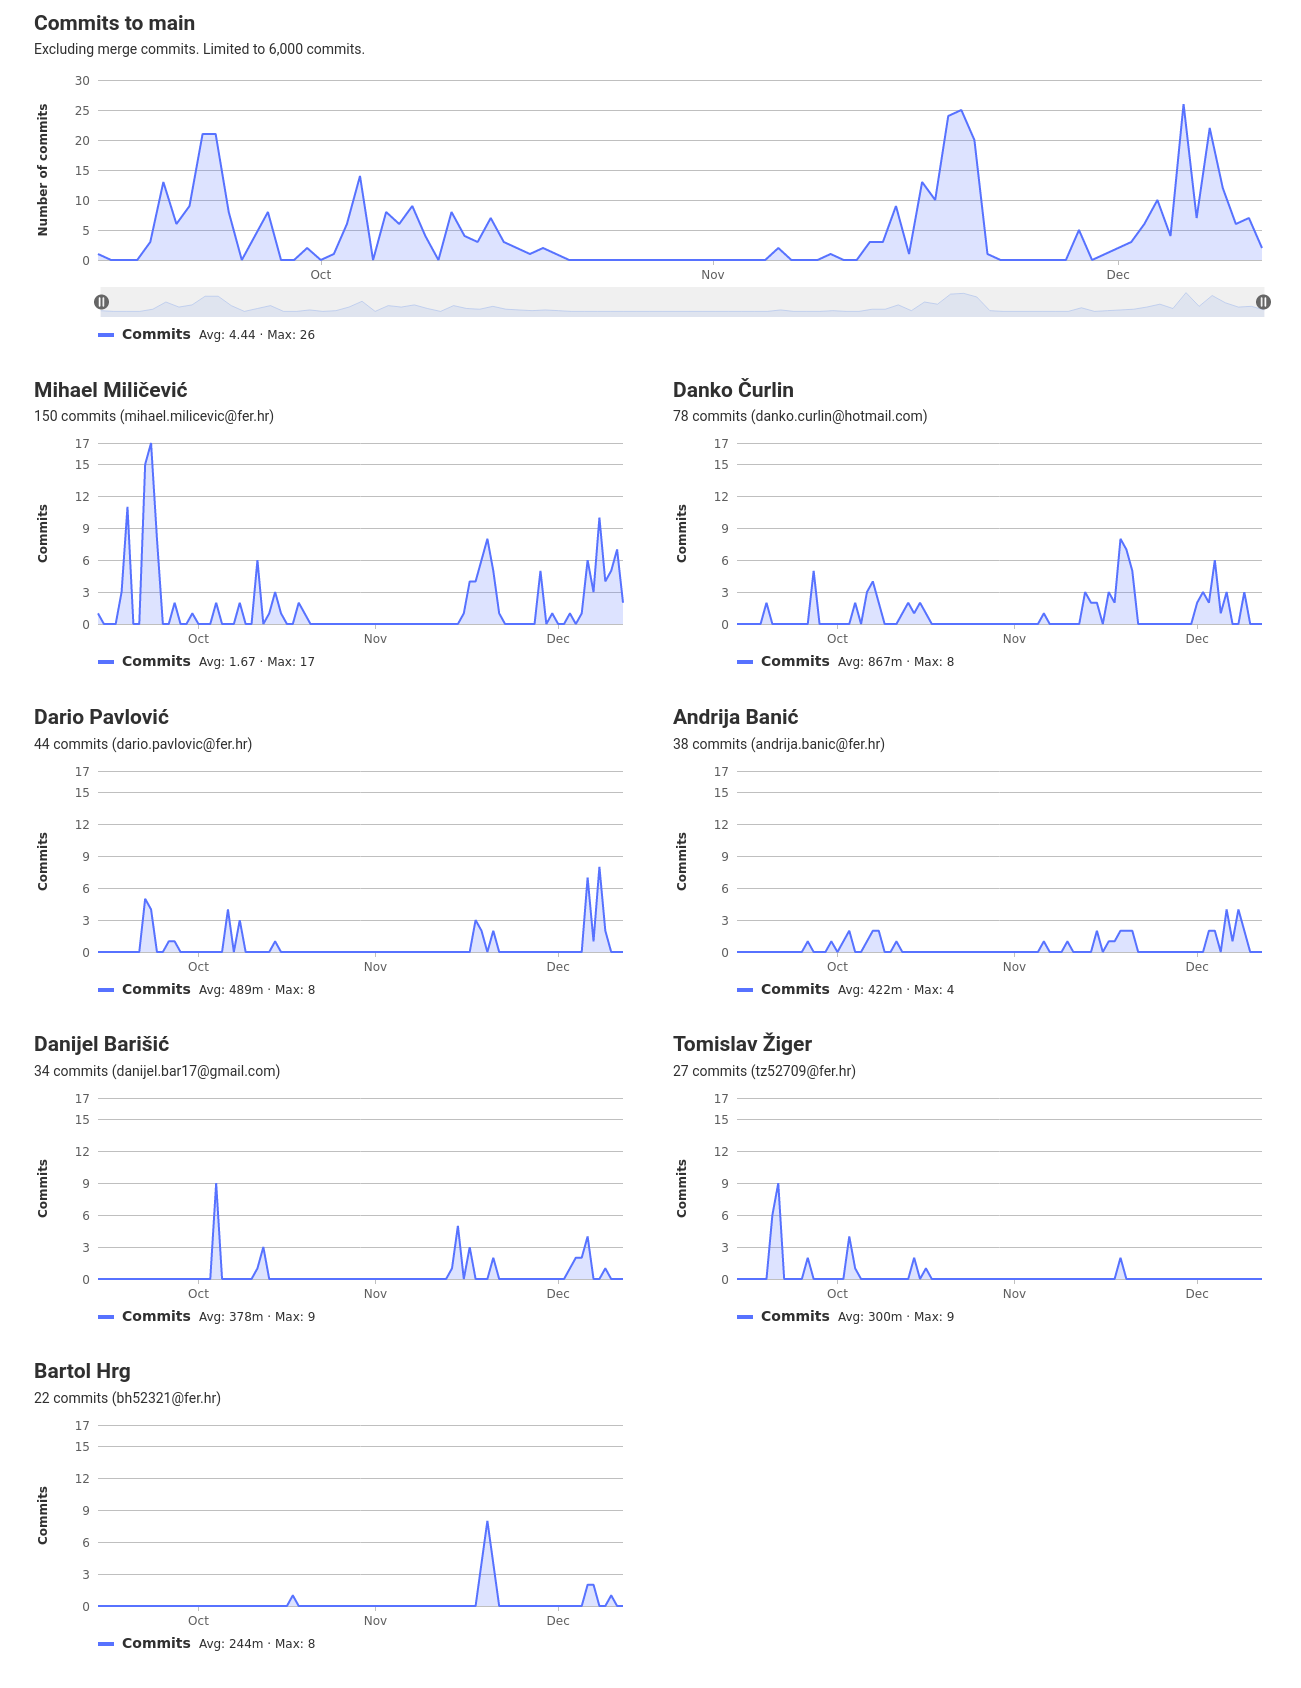
\includegraphics[width=\textwidth,keepaspectratio]{24 aktivnost u repozitoriju.png}
					\caption{Prikaz aktivnosti u repozitoriju}
				\end{figure}	
		
	


\end{document} %naredbe i tekst nakon ove naredbe ne ulaze u izgrađen dokument 


